%%***********************************************
%% Plantilla para TFM.
%% Escuela Técnica Superior de Ingenieros Informáticos. UPM.
%%***********************************************

%%-----------------------------------------------
%% Importar Preámbulo:
% -*-coding: utf-8 -*-
%%***********************************************
%% Plantilla para TFG.
%% Escuela Técnica Superior de Ingenieros Informáticos. UPM.
%%***********************************************
%% Preámbulo del documento.
%%***********************************************
\documentclass[a4paper,11pt,twoside]{book}
\usepackage[utf8]{inputenc}
\usepackage[T1]{fontenc}
\usepackage[english,spanish,es-lcroman,es-tabla]{babel}
\usepackage{bookman}
\decimalpoint
\usepackage{graphicx}
\usepackage{amsfonts,amsgen,amsmath,amssymb}
\usepackage[top=3cm, bottom=3cm, right=2.54cm, left=2.54cm]{geometry}
\usepackage{afterpage}
\usepackage{colortbl,longtable}
\usepackage{pdfpages}
\usepackage[hyphens]{url}
\usepackage[pdfborder={0 0 0}]{hyperref} 
\usepackage[stable]{footmisc}
\usepackage{parskip} % para separar párrafos con espacio.
%%-----------------------------------------------
% No estaban en la plantilla originalmente
\usepackage{multicol,multirow}
\usepackage{wasysym}
\usepackage{etoolbox}
\usepackage[inline]{enumitem}
\usepackage[acronym,toc,shortcuts]{glossaries}
\makeglossaries
\usepackage[
    sorting=none,
    style=numeric,
    defernumbers=true,
]{biblatex}
\addbibresource{include/all-references.bib}
\usepackage{csquotes}
\usepackage{subcaption}
\usepackage{wrapfig}
\usepackage{sidecap}
% \usepackage{minted}
% \setminted{
%     frame=lines,
%     framesep=2mm,
%     %  bgcolor=LightGray,
%     fontsize=\footnotesize,
%     linenos,
% }
\usepackage{float}
\newfloat{code}{thp}{lop}[chapter]
\floatname{code}{Código}
\usepackage{booktabs}
\usepackage{threeparttable}
\usepackage{datetime2}
\usepackage{siunitx}

\DeclareBibliographyCategory{cited}
\AtEveryCitekey{\addtocategory{cited}{\thefield{entrykey}}}

% TODO: Remove before submission
% \usepackage[left,pagewise]{lineno}
% \linenumbers
%%-----------------------------------------------
\usepackage{fancyhdr}
\pagestyle{fancy}
\fancyhf{}
\fancyhead[LO]{\leftmark}
\fancyhead[RE]{\rightmark}

% TODO: Remove before submission
% \fancyfoot[R]{\footnotesize Versión \DTMnow}

\setlength{\headheight}{1.5\headheight}
\cfoot{\thepage}

\addto\captionsspanish{ \renewcommand{\contentsname}
  {Tabla de contenidos} }
\setcounter{tocdepth}{4}
\setcounter{secnumdepth}{4}

\renewcommand{\chaptermark}[1]{\markboth{\textbf{#1}}{}}
\renewcommand{\sectionmark}[1]{\markright{\textbf{\thesection. #1}}}
\newcommand{\HRule}{\rule{\linewidth}{0.5mm}}
\newcommand{\bigrule}{\titlerule[0.5mm]}

\usepackage{appendix}
\renewcommand{\appendixname}{Anexos}
\renewcommand{\appendixtocname}{Anexos}
%\renewcommand{\appendixpagename}{Anexos}
\DeclareCaptionFormat{source}{%
  \ifx\captionsource\relax\relax\else
    \captionsource\par
  \fi
  #1#2#3\par}
\newcommand*\setcaptionsource[1]{\def\captionsource{{\footnotesize\textit{Fuente:}~#1}}}
\let\captionsource\relax
\captionsetup{format=source}

\setcounter{secnumdepth}{3} % Niveles numerados hasta subparagraph
\setcounter{tocdepth}{3}    % Niveles incluidos en el índice hasta subparagraph
%%-----------------------------------------------
%% Páginas en blanco sin cabecera:
%%-----------------------------------------------
\usepackage{dcolumn}
\newcolumntype{.}{D{.}{\esperiod}{-1}}
\makeatletter
\addto\shorthandsspanish{\let\esperiod\es@period@code}

\def\clearpage{
  \ifvmode
    \ifnum \@dbltopnum =\m@ne
      \ifdim \pagetotal <\topskip
        \hbox{}
      \fi
    \fi
  \fi
  \newpage
  \thispagestyle{empty}
  \write\m@ne{}
  \vbox{}
  \penalty -\@Mi
}
\makeatother
%%-----------------------------------------------
%% Estilos código de lenguajes: Consola, C, C++ y Python
%%-----------------------------------------------
\usepackage{color}

\definecolor{gray97}{gray}{.97}
\definecolor{gray75}{gray}{.75}
\definecolor{gray45}{gray}{.45}

\usepackage{listings}
\lstset{ frame=Ltb,
     framerule=0pt,
     aboveskip=0.5cm,
     framextopmargin=3pt,
     framexbottommargin=3pt,
     framexleftmargin=0.4cm,
     framesep=0pt,
     rulesep=.4pt,
     backgroundcolor=\color{gray97},
     rulesepcolor=\color{black},
     %
     stringstyle=\ttfamily,
     showstringspaces = false,
     basicstyle=\scriptsize\ttfamily,
     commentstyle=\color{gray45},
     keywordstyle=\bfseries,
     %
     numbers=left,
     numbersep=6pt,
     numberstyle=\tiny,
     numberfirstline = false,
     breaklines=true,
   }
\lstnewenvironment{listing}[1][]
   {\lstset{#1}\pagebreak[0]}{\pagebreak[0]}

\lstdefinestyle{consola}
   {basicstyle=\scriptsize\bf\ttfamily,
    backgroundcolor=\color{gray75},    
    }

\lstdefinestyle{CodigoC}
   {basicstyle=\scriptsize,
	frame=single,
	language=C,
	numbers=left
   }
   
\lstdefinestyle{CodigoC++}
   {basicstyle=\small,
	frame=single,
	backgroundcolor=\color{gray75},
	language=C++,
	numbers=left
   }

\lstdefinestyle{Python}
   {language=Python,    
   }
\makeatother   
%%-----------------------------------------------
%% Cargar datos relativos al TFM:
%% (actualizar estos datos en secciones/_DatosTFM.tex) 
%%***********************************************
%% Plantilla para TFM.
%% Escuela Técnica Superior de Ingenieros Informáticos. UPM.
%%***********************************************
%% Información requerida para completar la portada.
%%*********************************************** 

%% Escribe Nombre y Apellidos del autor del trabajo:
\newcommand{\NombreAutor}{David Davó Laviña}

%% Escribe el Grado: 
\newcommand{\Master}{Inteligencia Artificial}

%% Escribe el Título del Trabajo:
\newcommand{\TituloTFM}{Exploración de Sistemas Recomendadores para la Recomendación de Propuestas en Organizaciones Autónomas Descentralizadas} 

%% Escribe Nombre y Apellidos del Tutor del trabajo: 
\newcommand{\NombreTutorUCM}{Javier Arroyo}
\newcommand{\NombreTutorUPM}{Damiano Zanardini} 

% Escribe el Departamento al que pertenece el Tutor:
\newcommand{\DepartamentoUCM}{Ingeniería del Software e Inteligencia Artificial}
\newcommand{\DepartamentoUPM}{Inteligencia Artificial}

% Escribe la fecha de lectura, en formato: Mes - Año
\newcommand{\Fecha}{Mayo 2024}
%%***********************************************

% Cargar datos del glosario
% ----------------
% Definición de Acrónimos
% ----------------
% Add new key for long Spanish form:
\glsaddkey
{longsp}% key
{}% default value
{\glsentrylongsp}% new command analogous to \glsentrylong
{\Glsentrylongsp}% new command analogous to \Glsentrylong
{\acrlongsp}% new command analogous to \acrlong
{\Acrlongsp}% new command analogous to \Acrlong
{\ACRlongsp}% new command analogous to \ACRlong

% Add new key for plural long Spanish form:
\glsaddkey
{longplsp}% key
{}% default value
{\glsentrylongplsp}% new command analogous to \glsentrylongpl
{\Glsentrylongplsp}% new command analogous to \Glsentrylongpl
{\acrlongplsp}% new command analogous to \acrlongpl
{\Acrlongplsp}% new command analogous to \Acrlongpl
{\ACRlongplsp}% new command analogous to \ACRlongpl

\glsaddstoragekey
{baselang}
{\languagename}
{\glsentrylang}

% Provide conditional to test if longsp/longplsp has been set
\newcommand*{\glsifhaslongsp}[3]{%
  \ifcsempty{glo@#1@longsp}{#3}{#2}%
}
\newcommand*{\glsifhaslongplsp}[3]{%
  \ifcsempty{glo@#1@longplsp}{#3}{#2}%
}

% Define new acronym style:

\newacronymstyle{spanish}
{% base the display style on 'long-short'
  \GlsUseAcrEntryDispStyle{long-short}%
}%
{% base the definitions on 'long-short'
  \GlsUseAcrStyleDefs{long-short}%  
% Make some custom modifications for the first use display.
% Singular, no case change:
  \renewcommand*{\genacrfullformat}[2]{%
   \glsifhaslongsp{##1}%
   {% has Spanish version:
      \glsentrylongsp{##1}##2\space
      (\firstacronymfont{\glsentryshort{##1}}, \glsentrylong{##1})%
   }%
   {%
     \glsentrylong{##1}##2\space
     (\firstacronymfont{\glsentryshort{##1}})%
   }%
  }%
% Singular, first letter upper case:
  \renewcommand*{\Genacrfullformat}[2]{%
   \glsifhaslongsp{##1}%
   {% has Spanish version:
      \Glsentrylongsp{##1}##2\space
      (\firstacronymfont{\glsentryshort{##1}}, \glsentrylong{##1})%
   }%
   {%
     \Glsentrylong{##1}##2\space
     (\firstacronymfont{\glsentryshort{##1}})%
   }%
  }%
% Plural, no case change:
  \renewcommand*{\genplacrfullformat}[2]{%
   \glsifhaslongplsp{##1}%
   {% has Spanish version:
      \glsentrylongplsp{##1}##2\space
      (\firstacronymfont{\glsentryshortpl{##1}}, \glsentrylongpl{##1})%
   }%
   {%
     \glsentrylongpl{##1}##2\space
     (\firstacronymfont{\glsentryshortpl{##1}})%
   }%
  }%
% Plural, first letter upper case:
  \renewcommand*{\Genplacrfullformat}[2]{%
    \glsifhaslongplsp{##1}%
    {% has Spanish version:
      \Glsentrylongplsp{##1}##2\space
      (\firstacronymfont{\glsentryshortpl{##1}}, \glsentrylongpl{##1})%
    }%
    {%
      \Glsentrylongpl{##1}##2\space
      (\firstacronymfont{\glsentryshortpl{##1}})%
    }%
  }%
}

% switch to the new style:
\setacronymstyle{spanish}

% Define a new glossary style that checks for the existence of
% the longsp field.
\newglossarystyle{listsp}{%
  \setglossarystyle{list}% base style on the list style
  \renewcommand*{\glossentry}[2]{%
  \item[\glsentryitem{##1}%
        \glstarget{##1}{\glossentryname{##1}}]
    \edef\entrylang{\glsentrylang{##1}} % Needed to expand the macro
    \ifdefstrequal{\entrylang}{\languagename}{%
        \glossentrydesc{##1}%
    }{%
        \foreignlanguage{\glsentrylang{##1}}{\emph{\glossentrydesc{##1}}}%
    }%
    \glsifhaslongsp{##1}{\space(\glsentrylongsp{##1})}{}%
    \glspostdescription\space ##2}%
  \renewenvironment{theglossary}{
    \small
    \setlength{\columnsep}{.7cm}
    \begin{multicols*}{2}
    \begin{description}
  }{
    \end{description}
    \end{multicols*}
  }
}

% https://patorjk.com/software/taag/#p=display&f=Letters&t=A
%   AAA   
%  AAAAA  
% AA   AA 
% AAAAAAA 
% AA   AA 

% BBBBB   
% BB   B  
% BBBBBB  
% BB   BB 
% BBBBBB  
\newacronym[
    baselang=english,
    longsp={Representación de Codificador Bidireccional de Transformers},
]{bert}{BERT}{Bidirectional Encoder Representations from Transformers}
\newacronym[
    baselang=english,
    longsp={Comunidad Open-Source basada en Blockchain},
    longplsp={Comunidades Open-Source basadas en Blockchain},
]{boc}{BOC}{Blockchain-based Open-source Community}
\newacronym[
    baselang=english,
]{bpr}{BPR}{Bayesian Personalized Ranking}
        
%  CCCCC  
% CC    C 
% CC      
% CC    C 
%  CCCCC  
\newacronym[
    baselang=english,
    longsp={Filtrado Colaborativo},
]{cf}{CF}{Collaborative Filtering}
\newacronym[
    baselang=english,
    longsp={Trabajo Cooperativo Asistido por Computadora}
]{cscw}{CSCW}{Computer-Supported Cooperative Work}
\newacronym[
    baselang=english,
    longsp={Valores Separados por Comas},
]
{csv}{CSV}{Comma-separated values}
\newacronym[
    baselang=english,
]{ctdg}{CTDG}{Continuous-time dynamic graphs}
        
% DDDDD   
% DD  DD  
% DD   DD 
% DD   DD 
% DDDDDD  
\newacronym[
    % see={[Ver:]{dao-gls}},
    longsp={Organización Autónoma Descentralizada},
    longplsp={Organizaciones Autónomas Descentralizadas},
    baselang=english,
]{dao}{DAO}{Decentralized Autonomous Organization}
\newacronym[
    longsp={Aplicación Descentralizada},
    longplsp={Aplicaciones Descentralizadas},
    baselang=english,
]{dapp}{dApp}{Decentralized Application}
\newacronym[
    baselang=english,
    longsp=Ganacia Acumulativa Descontada
]{dcg}{DCG}{Discounted Cumulative Gain}
\newacronym[
    baselang=english,
    longsp={Finanzas Descentralizadas},
]{defi}{DeFi}{Decentralized Finance}
\newacronym[
    baselang=english,
    longsp=Grafos dinámicos de tiempo discreto,
]{dtdg}{DTDG}{Discrete-time dynamic graphs}

% EEEEEEE 
% EE      
% EEEEE   
% EE      
% EEEEEEE 
\newacronym[
    baselang=english,
    longsp={Redes Sociales Basadas en Eventos}
]{ebsn}{EBSN}{Event-Based Social Networks}
\newacronym[
    baselang=english,
    longsp={Función de Distribución Acumulativa Empírica}
]{ecdf}{ECDF}{Empirical Cumulative Distribution Function}
\newacronym[
    baselang=english,
    longsp={Máquina Virtual de Ethereum},
]{evm}{EVM}{Ethereum Virtual Machine}
        
% FFFFFFF 
% FF      
% FFFF    
% FF      
% FF      
\newacronym[
    baselang=english,
]{fm}{FM}{Factorization Machine}
        
%   GGGG  
% GG   GG 
% G    
% G   GGG
% GG   GG 
%  GGGGGG 
\newacronym{gdo}{GdO}{Garantías de Origen renovable}
\newacronym[
    baselang=english,
]{gcn}{GCN}{Graph Convolutional Network}
\newacronym[
    baselang=english,
]{gnn}{GNN}{Graph Neural Network}
        
% HH   HH 
% HH   HH 
% HHHHHHH 
% HH   HH 
% HH   HH 
        
% IIIII   
%  III    
%  III    
%  III    
% IIIII   
\newacronym{ic}{IC}{Intervalo de Confianza}
\newacronym[
    baselang=english,
    longsp={Oferta inicial de criptomonedas},
]{ico}{ICO}{Initial Coin Offering}
\newacronym[
    baselang=english,
]{ipfs}{IPFS}{InterPlanetary File System}
\newacronym[
    baselang=english,
    longsp=Recuperación de la Información,
]{ir}{IR}{Information Retrieval}
\newacronym[
    baselang=english
]{itemcf}{ItemCF}{item-based collaborative filtering}
        
%     JJJ 
%     JJJ 
%     JJJ 
% JJ  JJJ 
%  JJJJJ  
        
% KK  KK  
% KK KK   
% KKKK    
% KK KK   
% KK  KK  
\newacronym[
    baselang=english,
    longsp={Estimación de Densidad del Núcleo},
]{kde}{KDE}{Kernel Density Estimate}
\newacronym[
    baselang=english,
    longsp={Gran Modelo de Lenguaje},
    longplsp={Grandes Modelos de Lenguaje},
]{llm}{LLM}{Large Language Model}
\newacronym[
    baselang=english,
    longsp={k~vecinos más cercanos}
]{knn}{kNN}{k-nearest neighbors}
        
% LL      
% LL      
% LL      
% LL      
% LLLLLLL 
\newacronym[
    baselang=english,
]{lda}{LDA}{Latent Dirichlet Allocation} 
\newacronym[
    baselang=english,
]{lgc}{LGC}{Light Graph Convolution}

% MM    MM 
% MMM  MMM 
% MM MM MM 
% MM    MM 
% MM    MM
\newacronym[
    baselang=english,
    longsp={Precisión Media Promedio}
]{map}{MAP}{Mean Average Precission}
\newacronym[
    baselang=english,
    longsp={Factorización de Matrices}
]{mf}{MF}{Matrix Factorization}
\newacronym[
    baselang=english,
    longsp={Aprendizaje Automático},
]{ml}{ML}{Machine Learning}
\newacronym[
    baselang=english,
    longsp={Curso en línea masivo y abierto}
    longplsp={Cursos en línea masivos y abiertos}
]{mooc}{MOOC}{Massive Online Open Course}
\newacronym{mp}{MP}{Más Popular}


% NN   NN 
% NNN  NN 
% NN N NN 
% NN  NNN 
% NN   NN 
\newacronym[
    baselang=english,
]{nb}{NB}{Naive Bayes}
\newacronym[
    baselang=english,
]{ncf}{NCF}{Neural Collaborative Filtering}
\newacronym[
    baselang=english,
    longsp={Ganacia Acumulativa Descontada Normalizada}
]{ndcg}{nDCG}{Normalized Discounted Cumulative Gain}
\newacronym[
    baselang=english,
    longsp={Token no fungible},
    longplsp={Tokens no fungibles},
]{nft}{NFT}{Non-Fungible Token}
\newacronym[
    baselang=english,
]{ngcf}{NGCF}{Neural Graph Collaborative Filtering}


%  OOOOO  
% OO   OO 
% OO   OO 
% OO   OO 
%  OOOO0  
\newacronym[
    baselang=english,
]{openpop}{OpenPop}{Open Proposals}
\newacronym[
    baselang=english,
    longsp={Software de Código Abierto},
    longplsp={Softwares de Código Abierto},
]
{oss}{OSS}{Open-Source Software}

% PPPPPP     
% PP   PP    
% PPPPPP     
% PP         
% PP         
\newacronym{pd}{PD}{Programación Dinámica}
\newacronym{pln}{PLN}{Procesamiento del Lenguaje Natural}
           
%  QQQQQ     
% QQ   QQ    
% QQ   QQ    
% QQ  QQ     
%  QQQQ Q    
           
% RRRRRR     
% RR   RR    
% RRRRRR     
% RR  RR     
% RR   RR    

% DEPRECATED
% \newacronym[
%     baselang=english,
%     longsp={Sistema Recomendador},
%     longplsp={Sistemas Recomendadores},
% ]{rs}{RS}{Recommender System}
           
%  SSSSS     
% SS         
%  SSSSS     
%      SS    
%  SSSSS     
\newacronym[
    baselang=english,
    longsp={Estado del arte},
]{sota}{SOTA}{State of the Art}
\newacronym[
    longplural={Sistemas Recomendadores},
]{sr}{SR}{Sistema Recomendador}
\newacronym[
    baselang=english,
]{svd}{SVD}{Single Value Decomposition}
\newacronym[
    baselang=english,
]{svm}{SVM}{Support Vector Machine}
           
% TTTTTTT    
%   TTT      
%   TTT      
%   TTT      
%   TTT      
           
% UU   UU    
% UU   UU    
% UU   UU    
% UU   UU    
%  UUUUU     
\newacronym[
    baselang=english
]{usercf}{UserCF}{user-based collaborative filtering}
           
% VV     VV  
% VV     VV  
%  VV   VV   
%   VV VV    
%    VVV     
\newacronym[
    baselang=english,
    longsp={poder de votación}
]{vp}{VP}{voting power}
\newacronym{vpp}{VPP}{Votos por Propuesta}
\newacronym{vpv}{VPV}{Votos por Votante}
           
% WW      WW 
% WW      WW 
% WW   W  WW 
%  WW WWW WW 
%   WW   WW  
           
% XX    XX   
%  XX  XX    
%   XXXX     
%  XX  XX    
% XX    XX   
           
% YY   YY    
% YY   YY    
%  YYYYY     
%   YYY      
%   YYY      
           
% ZZZZZ      
%    ZZ      
%   ZZ       
%  ZZ        
% ZZZZZ      


%%-----------------------------------------------
%% Documento:
\begin{document}
%%***********************************************
%% Plantilla para TFM.
%% Escuela Técnica Superior de Ingenieros Informáticos. UPM.
%%***********************************************
%% Portada. 
%%***********************************************
\begin{titlepage}

\begin{minipage}{0.15\linewidth}
\hspace*{-2.5cm}
\noindent

\includegraphics[scale=0.5]{include/EscUpm.png} \qquad\qquad
\end{minipage}
\begin{minipage}{0.7\linewidth}
\begin{center}
\huge{ Universidad Politécnica\\de Madrid }\\
\vspace*{0.5cm}
\Large{\textbf{Escuela Técnica Superior de \\
Ingenieros Informáticos}}
\end{center}
\end{minipage}
\begin{minipage}{0.2\linewidth}

\includegraphics[scale=0.5]{include/FacInformatica.png} 
\end{minipage}

\vspace*{1cm}
\begin{center}
\Large{Máster Universitario en  \Master{} }
\end{center}

\vspace*{1cm}
\begin{center}
\huge{ Trabajo Fin de Máster }
\end{center}

\vspace*{0.5cm}
\begin{center}
\huge\bfseries {  \TituloTFM{} } 
\end{center}

\vspace*{5cm}

\noindent
\large{Autor: \NombreAutor{} }\\
\large{Tutores: \NombreTutorUPM{} \& \NombreTutorUCM{} }


\vspace*{4cm}
\begin{center}
Madrid, \Fecha
\end{center}

%%--------------------------------
\cleardoublepage
\thispagestyle{empty}
%%--------------------------------
\noindent
Este Trabajo Fin de Máster se ha depositado en la ETSI Informáticos de la Universidad Politécnica de Madrid para su defensa.

\vspace*{4cm}
\noindent
\textit{Trabajo Fin de Máster}\\
\textit{Máster Universitario en} \Master{}

\begin{enumerate}
\item[\textit{Título:}] \TituloTFM{}
\end{enumerate}
\Fecha


\vspace*{3cm}

\noindent
\begin{tabular}{ll}
\textit{Autor:} & \NombreAutor{}  \\ 
\textit{Tutores:} & \NombreTutorUPM{} \\
                & \DepartamentoUPM{} \\
                & ETSI Informáticos\\
                & Universidad Politécnica de Madrid \\
                \\
                & \NombreTutorUCM{}  \\ 
                & \DepartamentoUCM{} \\
                & Facultad de Informática \\
                & Universidad Complutense de Madrid                
\end{tabular} 

\end{titlepage}


%%-----------------------------------------------
%% Numeración romana:
\frontmatter
%%-----------------------------------------------
\chapter*{Agradecimientos}

A mi pareja por estar siempre a mi lado, apoyarme en los momentos más difíciles y recordarme que es necesario descansar de vez en cuando.

A mi familia por su respaldo incondicional y por inspirarme a ser curioso e ingenioso.

A mis tutores actuales por su orientación, apoyo, y grandes ideas, fundamentales para empezar y terminar este trabajo. Y a todos los buenos profesores y educadores del pasado que creyeron en mí, sin los que no me habría sido posible llegar hasta aquí.

Al personal de la facultad: cafetería, limpieza, biblioteca, administración, mantenimiento, etc. por darnos un buen lugar en el que trabajar estando cómodos.

A todas las personas que resuelven dudas y preguntas desinteresadamente en foros y Discords y Slacks, y dejan tras de sí un rastro de conocimiento experto que no puede encontrarse en ninguna biblioteca.

A todos aquellos gigantes y hackers sobre los que se apoya nuestro trabajo.
\\[16pt]

Finalmente, al Instituto de Tecnología del Conocimiento por proporcionar los recursos computacionales necesarios para el desarrollo de este trabajo.

Partes de este Trabajo de Fin de Máster se han realizado bajo el proyecto \textquote{Evaluación de Organizaciones Autónomas Descentralizadas basadas en Blockchain para la gestión de proyectos DeFi, NFT y Metaverso}, \href{https://produccioncientifica.ucm.es/proyectos/551171/detalle}{PID2021-127956OB-I00}, financiado por el Ministerio de Ciencia e Innovación y cofinanciado por la Unión Europea.

\begin{flushright}
    Mis más sinceros agradecimientos
\end{flushright}

\chapter*{Resumen}

Las Organizaciones Autónomas Descentralizadas (\textit{Decentralized Autonomous Organizations, DAOs}) han surgido como un nuevo enfoque hacia la gobernanza colectiva, facilitado por la tecnología blockchain. Las DAOs fomentan procesos de votación democráticos, permitiendo a los miembros proponer y votar sobre propuestas, moldeando así colectivamente el futuro de la organización. Sin embargo, la efectividad y legitimidad de la toma de decisiones dentro de las DAOs puede verse afectada por la baja participación de los votantes, un desafío común con otras comunidades en línea y los sistemas de votación tradicionales. Dada el tiempo limitado de votación de cada propuesta, las técnicas convencionales en sistemas recomendadores son inadecuadas. Por esa razón, este Trabajo de Fin de Máster introduce el primer sistema de recomendación diseñado específicamente para DAOs. En particular, se han desarrollado nuevas técnicas de validación y una nueva linea base. Este enfoque ha sido probado en tres modelos: un primero basado en filtrado colaborativo que utiliza Redes Neuronales de Grafos para explotar el grafo bipartito miembro-propuesta formado por la votación en DAOs; un segundo basado en contenido que utilizando Procesamiento del Lenguaje Natural; y un tercer modelo híbrido que combina los resultados de los dos anteriores. Aunque el proyecto se ha realizado con la organización de Decentraland en mente, que gobierna colectivamente una plataforma de metaverso con más de 35~000 miembros y 2~000 propuestas votadas, también se ha probado y comparado con otras organizaciones con diferentes características. Estos resultados no solo demuestran el potencial de los sistemas de recomendación para mejorar la personalización de propuestas y mejorar la participación de los votantes en las DAOs, sino que también se alinean con las mejoras observadas en la participación de los usuarios en otros proyectos colaborativos en línea que han implementado sistemas similares. Además, el sistema de recomendación basado en GNN con restricciones temporales podría ser adaptado a contextos similares, como la recomendación de eventos.

\textbf{Palabras clave}: Organizaciones Autónomas Descentralizadas, Sistemas Recomendadores, Redes Neuronales de Grafos, Procesamiento de Lenguaje Natural, Blockchain

%%--------------
\newpage
%%--------------

\chapter*{Abstract}
\begin{otherlanguage}{english}
Decentralized Autonomous Organizations (DAOs) have emerged as a novel approach to collective governance, facilitated by blockchain technology. DAOs foster democratic voting processes, allowing members to put forward and vote on proposals, thereby collectively shaping the organization’s future. However, the effectiveness and legitimacy of decision-making within DAOs can be compromised by low voter turnout, a challenge shared with traditional online communities and voting systems. Given the limited lifespan of each proposal, conventional recommender system techniques are unsuitable. In response to these issues, this Master's Thesis introduces a recommender system specifically designed for DAOs. In particular, new validation techniques and a baseline had to be developed. The approach has been tested on three models, a model that leverages Graph Neural Networks (GNN) for collaborative filtering, effectively exploiting the member-proposal bipartite graph inherent in DAOs voting, a second one that utilizes Natural Language Processing as a content-based approach, and a third hybrid model that combines the results of the previous two. While the project has been made with the Decentraland DAO organization in mind, which collectively governs a metaverse platform with over 35,000 members and 2,000 proposals voted, it has also been tested on and compared with other organizations with different characteristics. We compare our approach with a baseline that recommends the most popular open proposals at the time of recommendation. These models accurately predict future voters, surpassing the proposed baseline. These results not only underscore the potential of recommender systems in enhancing voter participation within DAOs but also align with the observed improvements in user engagement in other online collaborative projects that have implemented similar systems. Furthermore, our GNN-based recommendation systems with temporal constraints could be adapted to other settings such as event recommendation.

\textbf{Keywords}: Decentralized Autonomous Organizations, Recommender Systems, Graph Neural Networks, Natural Language Processing, Blockchain
\end{otherlanguage}


%%%%%%%%%%%%%%%%%%%%%%%%%%%%%%%%%%%%%%%%%%%%%%%%%%%%%%%%%%%
%% Final del resumen. 
%%%%%%%%%%%%%%%%%%%%%%%%%%%%%%%%%%%%%%%%%%%%%%%%%%%%%%%%%%%
\tableofcontents
\listoffigures

%%-----------------------------------------------
%% Numeración arábiga:
\mainmatter
%%----------------------------------------------- 
% \part{Introducción}
\include{secciones/01_Introduccion}

% \part{Estado del arte}
\chapter{Fundamentos tecnológicos}

El objetivo de este capítulo es presentar una introducción y unos fundamentos sobre la tecnología que da soporte a las organizaciones sobre las que se ejecutará el sistema recomendador, pues se considera que es importante entender sus limitaciones y el valor de estas tecnologías.

\section{Blockchain}

Un \textit{blockchain} (cadena de bloques) es un libro contable o \textit{ledger} distribuido que almacena una lista de transacciones. Cada bloque está firmado digitalmente utilizando los datos del bloque anterior, formando una cadena de tal manera que, de modificar un bloque, cambiaría la firma de todos los posteriores. Al estar esta lista distribuida, si uno de los nodos que almacena la lista cambia los datos, se produciría una incongruencia que sería detectada por el resto de nodos, por lo que podemos considerar el blockchain como una base de datos distribuida e inmutable, a la que solo se le pueden añadir datos.

Para realizar una nueva operación, el usuario utiliza una clave privada para firmar la transacción y la envía a algún nodo que participe en la red para que verifique la firma utilizando su clave pública, y se añada a la cadena. Sin embargo, los nodos que participan en la red necesitan de cierta comisión para realizar la operación. El \textit{hash} de la clave pública es la dirección que identifica al usuario, y que deberá usarse para realizar una transferencia. El programa o dispositivo que almacena esta clave privada se le conoce como cartera o \textit{wallet}, por lo que es común utilizar indistintamente este término para identificar a los usuarios. Nótese que al igual que en otras plataformas hay ciertos usuarios con varias cuentas, en blockchain también hay usuarios con varios \textit{wallets}, es decir, varias direcciones.

Tras procesar todas las transacciones realizadas desde el comienzo de la cadena de bloques, se obtiene el estado actual, con las cantidades obtenidas por cada usuario.

En 2008, una persona o grupo de personas conocido por el seudónimo de Satoshi Nakamoto desplegó satisfactoriamente Bitcoin, creando así la primera criptomoneda. Años después, en 2015 se lanzaría Ethereum~\cite{tual_ethereum_2015}, un blockchain desarrollado por el programador Vitalik Buterin que añadiría la revolucionaria capacidad de desplegar aplicaciones descentralizadas.

El conjunto de nodos participantes en la red de Ethereum forma una máquina virtual determinista basada en pila conocida como \gls{evm}. Esta máquina virtual ejecuta contratos inteligentes o \textit{smart contracts} que son desplegados por los usuarios. En este caso, una dirección de Ethereum puede representar tanto a un usuario como a un contrato inteligente, pero como estos últimos tienen las mismas capacidades que cualquier usuario, no se suele realizar ninguna distinción y se les considera simplemente otro tipo de agentes dentro del sistema.

Los contratos inteligentes se programan en un lenguaje de alto nivel y son compilados a \textit{bytecode} turing-completo del \gls{evm}, por lo que aunque su binario es público, el código fuente no lo es. Es común publicar el código fuente y las opciones del compilador utilizado para que los usuarios puedan verificar que compila al binario desplegado. Al igual que en Bitcoin, los usuarios deben pagar una comisión a los nodos para que su interacción con el contrato inteligente sea ejecutada.

Una de las mayores aplicaciones de este tipo de contratos es \gls{defi}, con la que se ofrecen diversos instrumentos financieros: préstamos, bonos, bolsas de valores, \textit{crowdfunding}... Sin embargo, las aplicaciones descentralizadas no se limitan sólo a las finanzas, también hay aplicaciones de juegos, energía, salud, ciencia, multimedia, entre otras~\cite{wu_first_2021}.

Para facilitar su uso, las aplicaciones descentralizadas utilizan una interfaz web a la que cualquiera puede acceder y leer los datos, aunque es necesario una extensión de navegador que haga de cartera para poder interactuar.

\section{Organizaciones Autónomas Descentralizadas}

Una \acrfull{dao} es un sistema basado en blockchain que permite a un grupo de personas coordinarse y auto-gobernarse mediante contratos inteligentes, y cuya gobernanza es descentralizada~\cite{hassan_decentralized_2021}. El término fue inventado en 2014 por Vitalik Buterin, programador de Ethereum~\cite{buterin_daos_2014}.

En la práctica, una \gls{dao} es un conjunto de contratos inteligentes que permiten a un conjunto de usuarios votar en propuestas, que tienen como efecto el realizar transacciones con su tesorería común, aceptar nuevos miembros, o incluso hacer llamadas a otros contratos inteligentes. En algunas organizaciones, es posible realizar propuestas aunque no se sea miembro, aunque sólo los miembros pueden votar.

Estas organizaciones han sido utilizadas para diversos propósitos, como votar propuestas de micromecenazgo y asignar presupuestos para invertir en la comunidad de manera participativa, similar a los presupuestos participativos. Además, existen organizaciones encargadas de administrar protocolos descentralizados, como las DAOs de Uniswap o Decentraland, así como de realizar compras de gran valor de manera conjunta, como el caso destacado de ConstitutionDAO, que recaudó 47 millones de dólares para adquirir una de las copias de la constitución estadounidense~\cite{kastrenakes_crypto_2021}. También se encuentran organizaciones más pequeñas que sirven para gestionar y administrar colectivos de desarrolladores o artistas, adoptando una estructura similar a la de una cooperativa~\cite{pena-calvin_categorization_2023}.

Debido a que es posible que una única persona tenga múltiples direcciones, en lugar de utilizar el esquema de un voto por persona, la organización asigna un \gls{vp} a cada usuario. La manera de asignar el \gls{vp} varía en cada comunidad, pero puede estar vinculado a la aportación de capital, a la realización de trabajos previos, o incluso ser asignada mediante propuestas de petición de \gls{vp}.

Debido a la inherente transparencia de Ethereum, el resultado de la votación y qué votó cada uno de los usuarios es siempre visible. Aunque podría ofuscarse o, incluso, encriptarse, las plataformas lo muestran sin ningún problema en la interfaz web.

Para evitar tener que programar una DAO desde cero, surgieron distintas plataformas para facilitar su despliegue a través de plantillas y sin necesidad de conocimientos de programación~\cite{faqir-rhazoui_comparative_2021}, dando lugar a un auge en la creación de organizaciones, llegando actualmente a registrarse más de 3 millones de miembros activos y manejando más de 30 mil millones de dólares estadounidenses en sus tesorerías, según el portal de analíticas Deepdao~\cite{deepdao_ventures_ltd_deepdao_2023}.

Aun así, las comunidades sufren de distintos problemas de seguridad, eficiencia, efectividad, y descentralización~\cite{buterin_governance_2018,buterin_moving_2021}, que intentan paliar utilizando métodos de votación distintos a la mayoría absoluta o relativa~\cite{fan_insight_2023}. Estos sistemas pueden llegar a ser muy complejos y difíciles de comprender por los usuarios, dificultando la participación.

Algunas comunidades intentan paliar estas cuestiones con medios externos a la blockchain. Por ejemplo, una práctica común es discutir minuciosamente una propuesta en foros o chats antes de subir la propuesta formalmente a la plataforma, asegurándose así de que será aprobada. Sin embargo, se reduce la transparencia del sistema pues no toda la comunidad participa en dichos canales, y algunos de ellos son jardines vallados a los que es imposible acceder sin registro previo, dependientes de una entidad central. Otros sistemas de votación permiten \textit{delegar} tu poder de votación, confiando en el juicio de individuos de confianza. En ambos casos, es necesario que al menos un usuario asuma la responsabilidad de estar al tanto de todas las propuestas, filtrarlas, y difundir su información o actuar de manera congruente. La ausencia de este usuario en momentos críticos de votación, o su decisión de modificar radicalmente su postura, podría desencadenar consecuencias adversas para la organización. Por ejemplo, si se lleva a cabo una votación para remunerar a un individuo que ha contribuido a la DAO, y dicha propuesta no obtiene aprobación, la confianza de otros colaboradores puede disminuir, desincentivando futuras colaboraciones.

Para mejorar la participación y disminuir los efectos del precio de Ethereum en la comunidad~\cite{faqir-rhazoui_effect_2021}, se ha buscado utilizar cadenas alternativas compatibles con la \gls{evm} y, por lo tanto, compatibles con el código de los contratos inteligentes desarrollados previamente. Estas cadenas suelen tener unos costes de operación menores, y un tiempo de bloque menor (es decir, tarda menos en ejecutarse cada operación), o están basadas en criptomonedas con precios estables, mejorando notablemente la usabilidad y obteniendo una rápida adopción.

\begin{figure}[t]
    \centering
    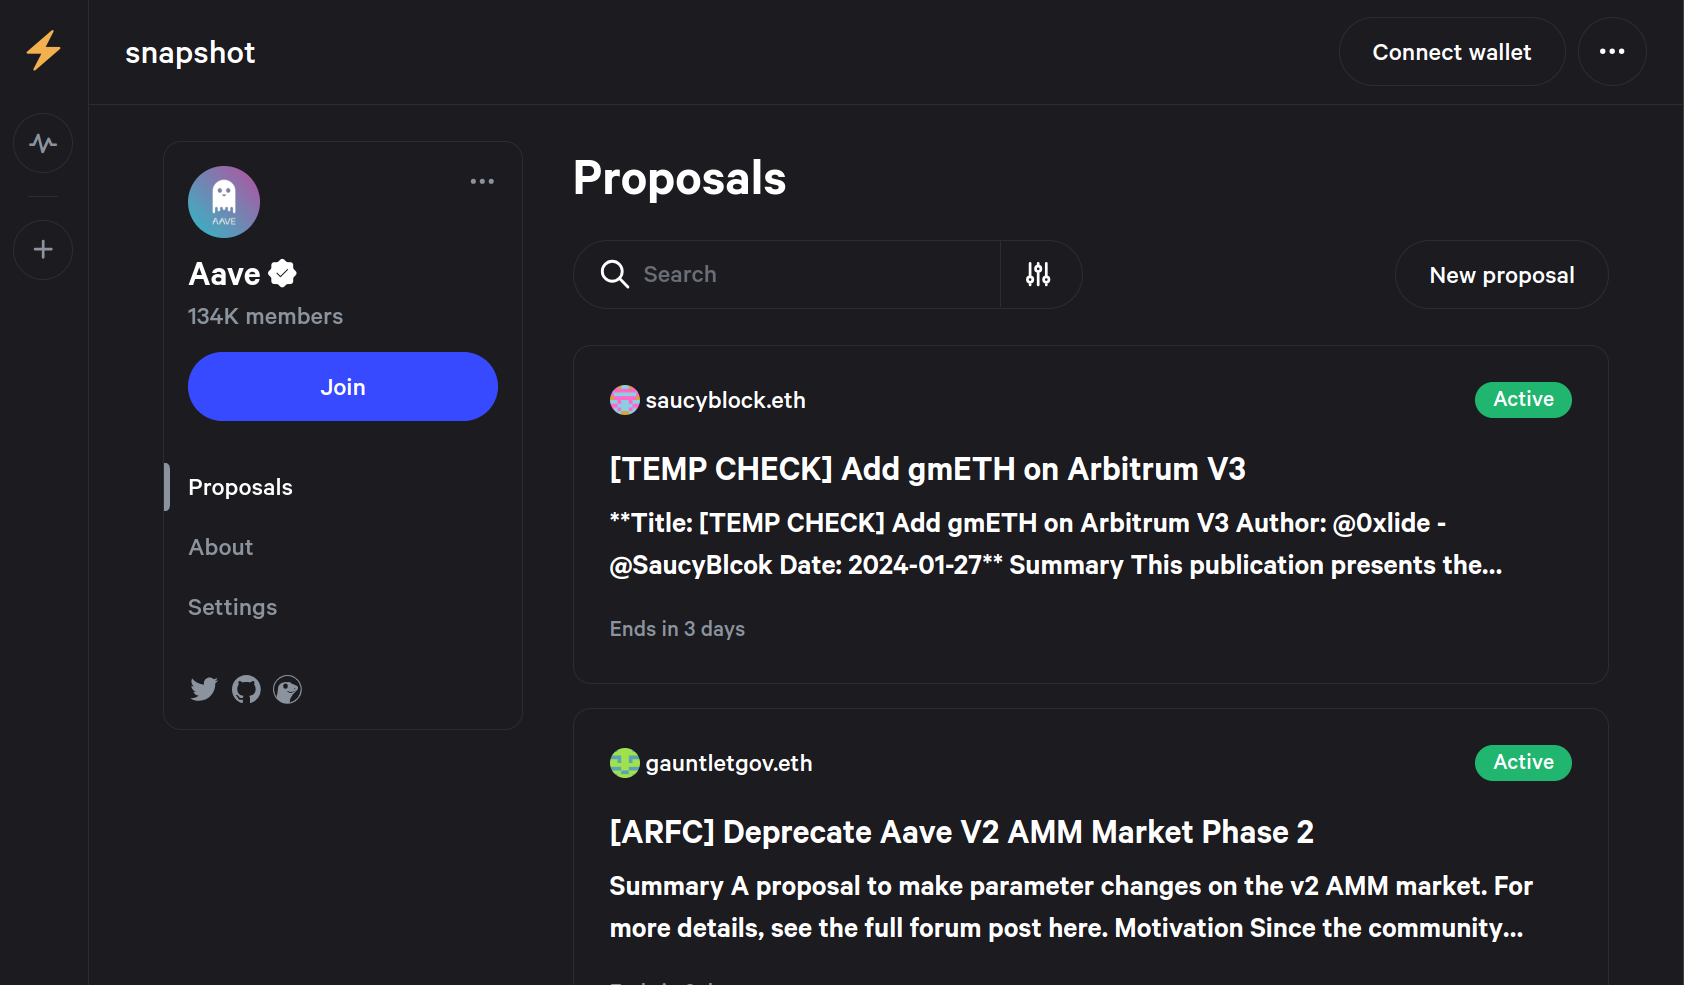
\includegraphics[width=\linewidth]{figures/02_sota/brave_screenshot_snapshot.org_aave.png}
    \setcaptionsource{\url{https://snapshot.org/\#/aave.eth}}
    \caption{Captura de pantalla de la interfaz web de la plataforma Snapshot para la gobernanza de la organización Aave.}
    \label{fig:screenshot_snapshot-gui}
\end{figure}

Finalmente, en 2021 se lanzó la plataforma \textit{off-chain} y, por lo tanto, sin costes de operación, pero manteniendo la seguridad y descentralización necesarias para las DAOs llamada Snapshot. Para mantener la descentralización, los votos están firmados digitalmente usando la clave privada del usuario, y tanto la interfaz como los resultados son almacenados en \gls{ipfs}, un protocolo de hipertexto descentralizado. Sigue teniendo las mismas capacidades de conectarse con una tesorería, realizar transferencias y ejecutar cualquier contrato inteligente, por lo que a efectos prácticos es como una DAO sin blockchain y mejor usabilidad. En la figura~\ref{fig:screenshot_snapshot-gui} se muestra una captura de la interfaz web.

Esta plataforma elevó en varios órdenes de magnitud el alcance de las DAOs, alojando actualmente más de 30 mil organizaciones que suman más de 3 millones de usuarios y 200 mil propuestas realizadas~\cite{pena-calvin_census_2024}.

\chapter{Sistemas Recomendadores}

\section{Trabajo relacionado}

Hasta donde sabemos, hasta ahora nadie ha estudiado el uso de Sistemas Recomendadores para \glspl{dao}. Por lo tanto, en esta sección se proporcionará una visión general de la aplicación de Sistemas Recomendadores en áreas cercanas.

Los Sistemas Recomendadores han sido usados para abordar el problema de la participación en proyectos colaborativos. Por ejemplo, en Wikipedia se han usado para recomendar tareas y artículos para traducir. SuggestBot, uno de los primeros de estos sistemas desplegado en 2007, realiza asignación de tareas (limpieza, arreglar formato, eliminar o fusionar artículos...) de manera personalizada usando filtrado colaborativo~\cite{cosley_suggestbot_2007}. Para llenar las lagunas en la traducción de artículos de manera eficiente y recomendar artículos que crear en otros idiomas, \cite{wulczyn_growing_2016} ordena los artículos por relevancia en cada idioma y después los asigna a editores basándose en el texto de sus contribuciones previas. WikiRecNet~\cite{moskalenko_scalable_2020} es un sistema creado sobre \textit{representation learning}, con \textit{Doc2Vec} y \textit{GraphSAGE} (una \gls{gcn}) para ayudar a los editores a lidiar con el gran volumen de artículos potenciales que pueden requerir de su atención. Notablemente, estos sistemas consiguieron satisfactoriamente mejorar las contribuciones de los miembros. 

Este tipo de sistemas también han sido usados en plataformas de desarrollo colaborativo como Bugzilla o GitHub para realizar triaje de \textit{bugs}, inicialmente en 2004 utilizando \textit{Naïve Bayes}~\cite{cubranic_automatic_2004}, y más recientemente utilizando técnicas más modernas como \textit{Hierarchical Attention Networks}~\cite{he_automatic_2021}. Estos sistemas también se han usado para ampliar el número de revisores recomendando desarrolladores adecuados que hayan trabajado en los mismos ficheros o similares~\cite{strand_using_2020,chueshev_expanding_2020,constantino_dual_2023} e incluso teniendo en cuenta el tiempo como contexto para realizar la recomendación usando \gls{gnn}~\cite{xie_time-series_2022}, o asignar \textit{bugs} a desarrolladores basándose en elementos textuales de \textit{bugs} arreglados en el pasado~\cite{sajedi-badashian_vocabulary_2020,diamantopoulos_automated_2023}, entre otras muchas tareas.

Por otro lado, podemos coger inspiración del uso de sistemas recomendadores en democracia electrónica o \textit{e-Democracy}. En elecciones tradicionales en las que se elige un partido o candidato en un momento concreto, se han utilizado \textit{Voting Advice Applications} para abordar el problema de la participación~\cite{garzia_research_2016}. Sin embargo, estas aplicaciones principalmente asisten al usuario a elegir un candidato próximo a sus tendencias y preferencias~\cite{garzia_voting_2019}. Por ejemplo, \textcite{teran_fuzzy_2010} provee información sobre candidatos próximos a las tendencias del usuario, y \textcite{buryakov_using_2022} utiliza datos abiertos del gobierno para facilitar la creación automática de estos sistemas, que normalmente utilizan datos de encuestas. En cambio, nuestro sistema trataría de recomendar propuestas que los usuarios puedan encontrar interesantes, sin dirigir a los usuarios hacia una opción en concreto de la propuesta, y sin tener en cuenta sus elecciones anteriores. 

El trabajo más cercano en este propósito sería el uso de sistemas recomendadores en plataformas de participación ciudadana~\cite{cantador_personalized_2017} y presupuestos participativos~\cite{cantador_whats_2018}. En estas plataformas los ciudadanos deciden qué propuestas la administración debería priorizar, normalmente las que cuentan con más apoyos. Las propuestas que son ignoradas no tienen impacto, mientras que en el contexto de las DAOs todas las propuestas deberían ser tenidas en cuenta. Además, ha de tenerse en cuenta de que los usuarios no pueden votar en contra de una propuesta, y las propuestas suelen permanecer abiertas durante un tiempo indefinido o muy largo, pues su implementación suele llevarse a cabo en los próximos meses o años y no inmediatamente, a diferencia de en las DAOs.

Finalmente, la característica temporal de las propuestas en las DAOs nos lleva al dominio de la recomendación de eventos en \gls{ebsn}, fijándonos sobre todo en la evaluación de dichos sistemas. \textcite{zhang_collective_2015} utilizan un modelo bayesiano, pero no parecen tener en cuenta el tiempo. \textcite{pham_general_2015} utilizan grafos heterogéneos y consideran el tiempo (día de la semana, hora del día) una parte esencial del contexto para realizar la recomendación, sin embargo, no se tiene el tiempo en cuenta a la hora de evaluar el sistema. \textcite{minkov_collaborative_2010} recomiendan conferencias científicas utilizando filtrado colaborativo. Se evalúa la recomendación de ítems de los que no existe feedback previo, y se realiza un estudio con usuarios obteniendo feedback explícito y simulando recomendaciones semanales. En el caso de feedback implícito, \textcite{macedo_context-aware_2015} realizan una especie de validación cruzada dividiendo los datos históricos en entrenamiento y test según un momento temporal. Sin embargo, estos sistemas tienden a depender demasiado del contexto para realizar las recomendaciones, mientras que en nuestro caso solo contamos con la información textual de las propuestas.

Cabe mencionar que, aunque sí se han utilizado técnicas de aprendizaje automático e inteligencia artificial para mejorar las aplicaciones basadas en blockchain~\cite{ressi_ai-enhanced_2024}, este parece ser el primer trabajo de aplicación de sistemas recomendadores a este tipo de organizaciones.

% En este capítulo de un par de páginas se desarrolla el estado del arte tanto en \glspl{sr}, como en DAOs, como en aplicaciones de las DAOs, y aplicaciones de sistemas a las DAOs, o aplicaciones de \glspl{sr} a DAOs. A continuación una lista placeholder con varios papers que he encontrado:

% \textbf{¿Qué hago con esto?} ¿Lo pongo en modo tabla como en~\cite{sajedi-badashian_vocabulary_2020}? ¿Lo pongo \textit{en texto plano}? ¿Itemizado? En caso de ser una tabla, tendría las siguientes columnas: Author, Year, Task (Bug Assignment, Bug Triage, Task Assignment), Técnicas usadas

% \begin{itemize}
%     \newcommand{\citesota}[1]{\textcite{#1}: \citetitle{#1} \citedate{#1}.}
%     \item \citesota{cubranic_automatic_2004} El paper más antiguo que he encontrado. Utiliza un \gls{nb} para asignar bug reports (texto) a desarrolladores. La clase a predecir por el NB es el developer al que asignar el bug.
%     \item Uno de los campos de uso más antiguos es el Automatic bug triage\cite{cubranic_automatic_2004, he_automatic_2021}, y el Bug Assignment~\cite{sajedi-badashian_vocabulary_2020}.
%     \item \citesota{castro-herrera_hybrid_2010} Crean un \gls{sr} híbrido para foros de herramientas Open Source (como KeePass, MikTex o Notepad++, entre otros), que recomienda a usuarios potenciales posts que aún no han sido respondidos. La línea base es una recomendación aleatoria (mucho más optimista), y miden precisión/recall y f2. (Es decir, no hacen ranking). Sin embargo, miran la precisión en k con k entre 1 y 200 (aunque en realidad a partir de 10 se estanca). Este autor ha explorado anteriormente otros sistemas para la recomendación en foros \cite{castro-herrera_recommender_2009-1}, y el uso de sistemas similares para la educción de requisitos (es decir, en la especificación de requisitos el hecho de pensar qué requisitos son necesarios) a gran escala. Este último sistema lo que hace es juntar a usuarios con intereses similares para que trabajen juntos.
%     \item \citesota{diamantopoulos_automated_2023} Utilizan topic modeling con \gls{lda} para asignar tickets JIRA automáticamente a los desarrolladores, no solo de bugs, sino también de nuevas caracteríticas, soporte, documentación, etc.
%     \item \citesota{chueshev_expanding_2020} Basandose en los ficheros modificados, recomienda reviewers a los pull requests realizados en sistemas de control de versiones, estos si que usan filtrado colaborativo (\gls{mf}).
%     \item \citesota{constantino_dual_2023} Igual que \cite{chueshev_expanding_2020}, se basan en los ficheros modificados, pero en este caso recomiendan colaboradores, es decir, otros desarrolladores a los que podrías consultar sobre un fichero en común. Usan TF-IDF para recomendar ficheros que sean relevantes, y evitar recomendar cosas que sean modificadas por todo el mundo.
%     \item \citesota{cosley_suggestbot_2007}. Usa filtrado colaborativo para asignar tareas (limpieza, stubs, merges, añadir fuentes, expandir, o arreglar el formato) a editores de Wikipedia basado en intereses personalizados basado en la historia de contribuciones del usuario.
%     \item \citesota{wulczyn_growing_2016}. Recomiendan artículos que existen en un idioma pero no existen en otro, basado en su importancia general y en los intereses de los editores.
%     \item \citesota{moskalenko_scalable_2020} explora el uso de \glspl{gnn} y doc2vec para realizar recomendaciones de artículos de Wikipedia. La principal diferencia con Pinterest o YouTube es que hay muy poca participación. Por el momento, creo que este es el más similar a lo nuestro.
%     \item \citesota{sajedi-badashian_vocabulary_2020} Asignación de bugs de GitHub. Este paper incluye un buen SOTA del campo del bug assignment.
%     \item \citesota{greco_stackintheflow_2018} Un plugin del IDE que recomienda post de stack overflow relevantes cuando se produce un error. Para ello, genera una query basándose en el código del fichero, pero también aprende del usuario, viendo en cual de los resultados de la query tiende a hacer click.
%     \item \citesota{xie_time-series_2022}. Utilizan una \gls{gnn} con un random walk sesgado en el tiempo para explotar el grafo de una mailing list para recomendar mediante \textit{link prediction} a nuevos usuarios de una comunidad mentores que puedan ayudarles, e intentar mantener el engagement. Destacaría que el scope de los datasets utilizados no es muy distinto al de las \glspl{dao}. Sinceramente, esto es lo que me hubiese gustado haber hecho.
%     \item \citesota{yang_forum_2014} Utilizan un recomendador híbrido con factorización de matrices para recomendar a los estudiantes de \glspl{mooc} hilos de su interés
%     \item \citesota{hu_question_2008} Hacen un \gls{sr} de preguntas abiertas e importantes en webs como Yahoo Answers (aún no existía StackOverflow) a usuarios, haciendo user modeling.
%     \item \citesota{di_sipio_multinomial_2020} Usan MNB para predecir el topic que tendrá un repositorio y así recomendar posibles topics a un repositorio que no los tenga.
%     \item \citesota{yan_auto-suggest_2020} Utilizan una red neuronal recurrente que recomienda que operadores utilizar en Jupyter Notebooks durante la fase de preparación de datos (limpieza, unión de dataframes, filtrado, etc.). No es realmente cooperative work, pero es un uso curioso. NADA. LA DESCARTO PORQUE NO TIENE MUCHO QUE VER.
%     \item \citesota{qian_learning_2021} Los sistemas de recomendación de visualizaciones estaban basados en reglas, pero este propone un sistema basado en \gls{ml} con un modelo wide-and-deep.
%     \item \citesota{chua_mvr-rcm_2024} Crean un \gls{sr} para recomendar microvideos educativos de la plataforma YouTube a usuarios interesados, pero no encuentro en el paper información concreta sobre la implementación del \gls{sr}.
%     \item \citesota{khanal_systematic_2020} Un systematic literature review de sistemas recomendadores para e-learning.
%     \item \citesota{mcnee_recommending_2002} Prueban varios algoritmos para recomendar artículos de investigación basandose en la red de citas entre papers.
%     \item \citesota{teran_fuzzy_2010} Voting Assistance en eGovernment
%     \item \citesota{cantador_whats_2018} Recomendador para Decide Madrid! Este parece el más similar a lo nuestro.
% \end{itemize}

% \textbf{[Conclusión]} Sin embargo, el uso de \glspl{sr} en \glspl{dao} es completamente nuevo. Además, la princial diferencia con el resto de sistemas es que las propuestas cierran pasado un tiempo, y tiende a dependerse demasiado del contenido, a penas se explora el filtrado colaborativo. También, que abunda el uso de \glspl{sr} en los que se \textit{asigna}, es decir, se hace una recomendación utilizando solo la mejor recomendación, e ignorando completamente el resto.

\section{Librerías de sistemas recomendadores}

En esta sección se realiza una exploración de potenciales librerías de sistemas recomendadores para la implementación del sistema propuesto en este trabajo. Se han buscado librerías en \textit{GitHub} y \textit{Papers With Code}, desarrolladas en los lenguajes de programación Python y/o R, que cuenten con una sólida base de usuarios y una documentación exhaustiva, y que al mismo tiempo incorporen los algoritmos estado del arte. A ser posible, basados en \gls{gnn}.

A continuación se detallan las librerías consideradas durante esta exploración, sin seguir un orden específico:

\begin{description}
    \item [Spotlight~\cite{kula_spotlight_2017}] Con 2.9k estrellas en GitHub, es una de las librerías de sistemas recomendadores más famosas, actualmente está basada en PyTorch~\cite{paszke_pytorch_2019} y su objetivo es ser una herramienta para la exploración rápida y el prototipado de nuevos modelos, utilizando sus funciones de pérdida, herramientas de validación cruzada  y evaluación, o capas creadas. Sin embargo, también incluye implementaciones de modelos de factorización, basados en representaciones latentes, o incluso de secuencia. No obstante, no contiene modelos basados en grafos, y lleva 4 años sin recibir actualizaciones.
    \item [Surprise~\cite{hug_surprise_2020}] Es un scikit (add-on basado en SciPy~\cite{virtanen_scipy_2020}) para sistemas recomendadores que hace gala de su extensa documentación y comunidad, con 6k estrellas en GitHub. Tiene interfaces muy similares a las de scikit-learn, por lo que es fácil de aprender a usar, y cuenta con varios algoritmos de filtrado colaborativo y hace sencillo el implementar nuevos algoritmos. Sin embargo, no cuenta con nada para sistemas basados en contenido.
    \item [Implicit~\cite{frederickson_implicit_2018}] Como su nombre indica, esta librería se especializa en conjuntos de datos de feedback implícito como es nuestro caso. Su mayor fortaleza parece ser la rápida ejecución de sus modelos, algunos optimizados con código propio en CUDA. Sin embargo, al igual que surprise, no tiene ningún modelo basado en contenido.
    \item [Crab~\cite{caraciolo_crab_2010}] Es otro scikit como surprise, pero creado mucho tiempo antes, en 2010. No cuenta con actualizaciones desde hace 13 años, por lo que se ha descartado su uso para evitar problemas de compatibilidad de dependencias. Sin embargo, se mantiene en esta lista pues tiene pocas dependencias y la implementación de algunos de los algoritmos podría servir de material de referencia.
    \item [Pytorch Geometric~\cite{fey_fast_2019}] Su repositorio en GitHub cuenta con 20 mil estrellas, y está respaldada por la extensa comunidad de PyTorch~\cite{paszke_pytorch_2019}, por lo que contará con actualizaciones constantes a lo largo del tiempo. Aunque cuenta con muy buenas herramientas para \gls{gnn}, al comienzo de este trabajo no era factible usarla para sistemas recomendadores, pues habría que definir las métricas offline de evaluación, entre muchas otras cosas. En un principio se decidió usar esta librería, pero al tratarse de un nuevo conjunto de datos que no se ha probado anteriormente en sistemas recomendadores, con peculiaridades que lo hacen muy distinto a otros sistemas recomendadores (véase el capitulo~\ref{ch:planteamiento-problema}), se encontraron muchos problemas de desarrollo. Al tener que crear tanto código nuevo (conversión de datos a grafo, sampling, evaluación...), y tratarse de una librería en muy bajo nivel, era muy difícil depurar el código. En la versión 2.5.0 de febrero 2024 añadieron soporte para sistemas recomendadores, implementando métricas de recuperación como la precisión en $k$ o el \acrshort{ndcg}.
    \item [Recommenders: Best Practices on Recommendation Systems~\cite{argyriou_microsoft_2020}] (anteriormente Microsoft's Recommenders). Librería creada por Microsoft con implementación de varios modelos de filtrado colaborativo, basado en contenido e híbridos. También cuenta con funciones de preparación de datos, métricas de evaluación offline, y herramientas para el despliegue de los modelos en un entorno de producción en Azure. De entre todas las librerías exploradas, consideramos que esta es la más completa y más adecuada para nuestro caso de uso.
    \item [LibRecomender~\cite{massquantity_librecommender_2020}] Aunque su uso aún no está muy extendido y su versión 1.0 se lanzó en 2023, es una librería muy prometedora. Su enfoque integral abarca todo el proceso, desde el entrenamiento hasta el despliegue de los modelos. Cuenta con más de 20 modelos implementados en Tensorflow y PyTorch a su disposición, entre ellos muchos basados en \acrshort{gnn} como Deepwalk, LightGCN, NGCF o GraphSAGE, así como modelos híbridos que permiten tener en cuenta la información textual de las propuestas. También cuenta con soporte para características dinámicas y recomendaciones secuenciales. La única razón por la que no se eligió utilizar esta librería es porque se desconocía su existencia al comenzar el trabajo, y sólo se descubrió al realizar una revisión del estado del arte.
\end{description}

Finalmente, se decidió utilizar la librería Microsoft Recommenders~\cite{argyriou_microsoft_2020} para realizar un prototipado rápido y poder experimentar con varios modelos. Además, el repositorio cuenta con multitud de ejemplos de cada modelo que ilustran buenas prácticas y recomendaciones en el diseño de sistemas recomendadores.

\section{Modelos}

En esta sección se presentan los diferentes modelos de sistemas recomendadores que han sido considerados para este trabajo, junto con cierto contexto que permita la comprensión de su funcionamiento.

En sistemas recomendadores, podemos distinguir dos tipos de modelos según los datos con los que trabajen. Los modelos basados en \acrfull{cf} se basan en las interacciones entre usuarios e ítems para realizar las recomendaciones~\cite{aggarwal_recommender_2016}, mientras que los modelos basados en contenido utilizan otros atributos de los usuarios e ítems, tal como la información textual, etiquetas, o ubicación. Los modelos híbridos combinan ambos enfoques para mejorar las recomendaciones y reducir sus problemas.

Aunque también existen sistemas recomendadores basados en conocimiento, no se tratan en este trabajo debido a que es necesario cierta interactividad con la que no contamos.

% Se da tan por hecho que no he encontrado ningún sitio que explique implicit/explicit feedback tal cual o de una definición
Por otro lado, los sistemas recomendadores dependen de la fuente de los datos de entrada que se emplean para realizar las recomendaciones. En el \textit{feedback explícito} el usuario da una opinión directa sobre la interacción, como puede ser seleccionar \textquote{me gusta} o \textquote{no me gusta}, dar estrellas, o escribir una reseña. Por otro lado, en el \textit{feedback implícito} se observa el comportamiento del usuario, como puede ser el historial de acciones del usuario o el tiempo dedicado a un contenido~\cite{jawaheer_comparison_2010}. Como se detalla en el capítulo~\ref{ch:planteamiento-problema}, los datos utilizados en este trabajo son feedback implícito, por lo que en el resto de esta sección nos centraremos en modelos que acepten este tipo de datos.

\subsection{Filtrado colaborativo}
% Ver la librería de librecommender

La idea principal de este tipo de modelos es utilizar la similitud entre las preferencias de distintos usuarios. Los métodos de recomendación basados en filtrado colaborativo se pueden dividir en basados en memoria y basados en modelos.

En los métodos basados en memoria, también llamados basados en vecindario, el \textit{score} para cada par ítem-usuario se genera basándose en los vecinos inmediatos. En concreto, si se genera basándose en los ítems con los que interactúa cada usuario, se denomina \gls{usercf}, y si se utilizan los vecinos de cada ítem se denomina \gls{itemcf}.

Por otra parte, los métodos basados en modelos utilizan modelos de predicción basados en aprendizaje automático y minería de datos, aprendiendo los parámetros necesarios para minimizar una función de pérdida con unos datos de entrenamiento.

Las implementaciones más sencillas de \gls{itemcf} y \gls{usercf} con feedback explícito crean una matriz de ítems-ítems o usuarios-usuarios completa y completan los espacios vacíos de la matriz utilizando las similitudes entre filas, por ejemplo, mediante la similitud del coseno~\cite{massquantity_librecommender_2020}.

\subsubsection{Factorización de Matrices}

Para mejorar tanto la eficiencia como la calidad de las recomendaciones, se utilizan métodos de reducción de la dimensionalidad, representando los ítems y usuarios en un espacio latente de menos dimensiones. La principal familia de este tipo de métodos es la \gls{mf}, en la que la matriz original se descompone en matrices rectangulares tal que su producto sea similar a la matriz original~\cite{koren_matrix_2009}. Originalmente se propuso un método parecido a \gls{svd}~\cite{funk_netflix_2006}, que posteriormente fue mejorado como SVD++ teniendo en cuenta el \textit{bias} o sesgo de cada ítem o usuario para poder abordar también feedback implícito~\cite{koren_factor_2010}. Recientemente, se han propuesto técnicas de descomposición de matrices mediante arquitecturas no lineales, como \gls{ncf}~\cite{he_neural_2017} que utiliza redes neuronales.

\subsubsection{Modelos basados en grafos}

De entre todos los modelos de aprendizaje profundo para recomendación, consideramos los métodos basados en grafos para la tarea de filtrado colaborativo~\cite{wu_graph_2022}. En este tipo de modelos, se utilizan técnicas de \textit{embedding} de grafos para modelar las relaciones entre los nodos~\cite{wang_graph_2020}.
Los sistemas recomendadores tradicionales, como \gls{mf}, solo tienen en cuenta los elementos con los que el usuario interactúa directamente. En cambio, las \gls{gnn} utilizan información de un vecindario extendido. Esto les permite capturar relaciones más complejas y aprovechar mejor la información estructural~\cite{gao_survey_2023}. Se espera que este tipo de modelos puedan captar los matices de las relaciones presentes entre los miembros de la DAO, como lo han demostrado en tareas similares, como la identificación de usuarios malintencionados~\cite{dupont_new_2024}.

Uno de los sistemas pioneros en este campo es DeepWalk~\cite{perozzi_deepwalk_2014}, que utiliza paseos aleatorios para aprender la representación de nodos. 
Poco después surgieron las \acrfull{gcn}~\cite{duvenaud_convolutional_2015}, que combinan la convolución de grafos y las redes neuronales para profundizar en la estructura de los subgrafos con vecinos a varios saltos. GraphSAGE fue uno de los primeros modelos en seguir este enfoque~\cite{hamilton_inductive_2017}, y \gls{ngcf}~\cite{wang_neural_2019} introdujo los este tipo de redes al campo del filtrado colaborativo, logrando resultados estado del arte.
Para este proyecto, se decidió utilizar LightGCN, una popular modificación de \gls{ngcf}, debido a su simplicidad y buenos resultados en \textit{user-item collaborative filtering}, superando otros modelos basados en \gls{gcn} previos~\cite{he_lightgcn_2020}.

\paragraph{LightGCN}
\label{subsubsec:lightgcn}
está basado en el modelo \acrfull{ngcf}~\cite{wang_neural_2019}, pero se simplifica al eliminar las matrices de transformación de características que se aprenden en cada convolución. En su lugar, la operación de convolución de grafos (también conocido como regla de propagación), denominada \acrfull{lgc}, realiza una suma ponderada normalizada de los \textit{embeddings} de los vecinos, como se detalla en la ecuación~\ref{eq:3_lgc}

\begin{equation}\label{eq:3_lgc}
    e_u^{(k+1)} = \sum_{i\in \mathcal{N}_u} \frac{1}{\sqrt{\left|\mathcal{N}_u\right|}\sqrt{\left|\mathcal{N}_i\right|}} e_i^{(k)};
    \;
    e_i^{(k+1)} = \sum_{i\in \mathcal{N}_i} \frac{1}{\sqrt{\left|\mathcal{N}_i\right|}\sqrt{\left|\mathcal{N}_u\right|}} e_u^{(k)}
\end{equation}

Por lo tanto, los únicos parámetros entrenables del modelo son los de la primera capa, y la matriz de predicciones final es la media de los embeddings de cada capa, como se detalla en la ecuación~\ref{eq:3_lgcn_layers}. 

\begin{equation}\label{eq:3_lgcn_layers}
    e_u = \sum_{k=0}^{K} e_u^{(k)};\;
    e_i = \sum_{k=0}^{K} e_i^{(k)}
\end{equation}

La puntuación para una determinada interacción usuario-ítem será $y_u=e_u^\top e_i$. Dado que los únicos parámetros que son aprendidos son los de la primera capa del modelo, la complejidad de este algoritmo es similar a \gls{mf}, dependiente del número de dimensiones del espacio latente y el número total de usuarios e ítems. La arquitectura de este modelo queda definida por el número de dimensiones del espacio latente y el número de capas de convolución.

La función de pérdida utilizada por el modelo es \acrfull{bpr}~\cite{rendle_bpr_2012}. Creado para feedback implícito, en lugar de reemplazar las no-interacciones con ceros asumiendo que es equivalente a feedback negativo, se comparan muestras positivas y muestras negativas para cada usuario, buscando maximizar la probabilidad de que el usuario prefiera la muestra positiva frente a la negativa.

En este trabajo se ha utilizado la implementación de este modelo de la librería Microsoft Recommenders~\cite{argyriou_microsoft_2020}, aunque ha sido necesario modificarlo para tener en cuenta las propuestas cerradas añadiendo un post-filtrado, como se detalla en la subsección~\ref{subsec:implementacion-colaborativo}. El código modificado se encuentra disponible en el GitHub del proyecto~\cite{davo_daviddavoupm-tfm-notebooks_2024}.

\subsection{Filtrado basado en contenido}
\label{subsec:recsys-content}

Los sistemas basados en contenido se basan en los atributos del elemento a recomendar y el perfil de preferencias del usuario, que a su vez está basado en los atributos de elementos con los que ha interactuado en el pasado~\cite{aggarwal_recommender_2016}.

Este tipo de sistemas tienen una ventaja en el escenario de arranque en frío (\textit{cold-start}) en items, en el que aún no se tiene suficiente feedback de otros usuarios como para realizar buenas recomendaciones con filtrado colaborativo. En tal caso, con tener suficiente información para formar un buen perfil del usuario es suficiente. Sin embargo, estos sistemas no pueden realizar recomendaciones a nuevos usuarios, al no tener información con la que formar un perfil.

Un sistema recomendador basado en contenido generalmente sigue tres pasos: el preprocesado y extracción de atributos de los ítems, el aprendizaje de los perfiles de los usuarios, y finalmente el filtrado y recomendación.

En la extracción de atributos se crea un vector para cada elemento, y es un paso muy dependiente del dominio. Por ejemplo, con información textual, pueden usarse métodos clásicos como \textit{bag-of-words}, TF-IDF, o \textit{embeddings} preentrenados. El aprendizaje de los modelos de usuario es similar al campo de clasificación de texto, y se usan métodos similares como \gls{knn}, similitud del coseno, o clasificadores bayesianos. Finalmente, se utilizan los resultados del modelo anterior para realizar la recomendación, por ejemplo recomendando los $k$ ítems con mayor similitud al usuario, o que mayor probabilidad tienen de pertenecer a la clase de ítems interactuados. Este último paso suele ser muy eficiente y puede ejecutarse en tiempo real.

En la sección~\ref{subsec:implementacion-contenido} se explora la implementación usada en este trabajo, que hace uso de \textit{embeddings} preentrenados para las características, y explora varios métodos de creación del perfil del usuario. El código del modelo desarrollado se puede encontrar en el GitHub del proyecto~\cite{davo_daviddavoupm-tfm-notebooks_2024}.

\subsection{Híbridos}

Los sistemas híbridos permiten combinar múltiples fuentes de datos para realizar mejores recomendaciones. Según el diseño del sistema, podemos distinguir las siguientes maneras de desarrollar un sistema recomendador híbrido~\cite{aggarwal_recommender_2016}:

\begin{enumerate}
    \item \textbf{Diseño monolítico}: Se crea un sistema recomendador que integra varias fuentes de datos, sin que existan componentes individuales. Un ejemplo de estos sistemas son las \acrfull{fm}~\cite{rendle_factorization_2010}, que combinan las ventajas de los \glspl{svm} con la \acrlongsp{mf}~\cite{zhang_introduction_2022}.
    \item \textbf{Sistemas mixtos} Utilizan múltiples sistemas recomendadores preexistentes y se presentan sus resultados a los usuarios en paralelo.
    \item \textbf{Diseño de ensamblado} Al igual que en los sistemas mixtos, se utilizan varios sistemas recomendadores preexistentes que son combinados en una salida más robusta. El quid de este tipo de sistemas es elegir una metodología para combinar la salida de estos sistemas, que puede utilizar o bien los \textit{scores} de cada sistema o bien la posición de las recomendaciones realizadas.
\end{enumerate}

El sistema híbrido desarrollado en este trabajo es un sistema de ensamblado que combina los otros dos sistemas desarrollados utilizando la posición de sus recomendaciones, y su especificación se detalla en la sección~\ref{subsec:implementacion-hybrid}.

% \subsubsection{Factorization Machines}

% % TODO: Releer el abstract del paper y hacer esta sección
% Combinando las ventajas \gls{svm} y \gls{mf} se crean las \acrfull{fm}~\cite{rendle_factorization_2010}, que son aplicables a problemas de predicción genéricos con cualquier tipo de datos de entrada.

% \begin{itemize}
%     \item Factorization Machine??
%     \item DeepFM
%     \item LightFM
% \end{itemize}


% \part{Diseño e implementación}
\chapter{Planteamiento del problema}
\label{ch:planteamiento-problema}

% \begin{itemize}
%     \item Las \gls{dao} permiten a sus miembros tomar decisiones votando en propuestas.
%     \item Cualquier persona (sea miembro o no) puede realizar una propuesta
%     \item Pero solo los miembros pueden votarlas
%     \item Puede surgir un problema: mucha propuesta, poca participación
%     \item Solución propuesta: Crear un sistema recomendador
%     \item El sistema recomendador debe recomendar a \textbf{usuarios} \textbf{propuestas} (items) en las que \textbf{votar} (interactuar) dentro de una DAO.
%     \item En las \glspl{dao} normalmente no suelen entrar nuevos usuarios (no hay mucho problema de cold start en ese respecto)
%     \item Sin embargo, sí que entran continuamente nuevos ítems.
%     \item Además, hay restricciones temporales. No podemos recomendar una propuesta que esté cerrada.
%     \item El feedback del usuario es implícito (si no votó puede ser que estuviese interesado pero no la viese, o aun no tuviese poder de votación)
%     \item El usuario puede votar a favor o en contra, pero en ambos casos lo tratamos como una muestra positiva porque nos interesa recomendar propuestas que al usuario le interese votar, sin importar su opinión.
%     \item Además, importante, en una DAO el estado actual de la votación es visible en todo momento y no es anónimo (tal vez no vota por miedo, o porque ya no sirve de nada votar), pero ese es otro tema
%     \item Nuestro sistema sería parecido a un sistema recomendador de eventos u obras de teatro. No tiene sentido recomendar una obra de teatro si ya no está en cartelera.
% \end{itemize}

Las \gls{dao} permiten a sus miembros la toma de decisiones mediante el voto en propuestas. Si bien cualquier individuo, miembro o no, puede proponer, únicamente los miembros tienen el derecho de votar sobre estas propuestas. No obstante, la abundancia de propuestas y la baja participación plantean un desafío en el funcionamiento de estas organizaciones. En respuesta a esta problemática, se propone la implementación de un sistema recomendador. Este sistema tiene como objetivo sugerir a los usuarios propuestas en las cuales puedan interactuar dentro de una DAO, promoviendo así una mayor participación y compromiso por parte de los miembros.

Es importante resaltar que en algunas \glspl{dao} sin muchos miembros, no suelen unirse nuevos usuarios, la mayoría se unen en la creación de la \gls{dao}, por lo que el problema del \textit{cold-start} en los miembros no debería ser demasiado notable. Sin embargo, cada día se agregan varias propuestas que, además, tienen un tiempo de vida establecido, por lo que el sistema tendrá que lidiar continuamente con el problema de \textit{cold-start} con cada propuesta creada, y además no es conveniente realizar recomendaciones de propuestas que ya están cerradas, pues el usuario no podrá votar.

El usuario puede expresar su preferencia votando a favor o en contra de una propuesta, y ambas acciones se interpretan como una muestra positiva para el sistema recomendador. Es decir, se trata de feedback implícito~\cite{oard_implicit_1998}. Es relevante señalar que, dentro de una \glspl{dao}, el estado actual de la votación es transparente y no anónimo, lo que puede influir en el comportamiento de los usuarios y su decisión de participar en el proceso de votación. Si la propuesta ya tiene mayoría absoluta (o incluso una fuerte mayoría relativa), puede que el usuario no vote.

El sistema recomendador propuesto para \glspl{dao} sería similar a un sistema utilizado en otros contextos temporales, como eventos u obras de teatro, en el que no tiene sentido recomendar una obra que ya no está en cartelera, pues el usuario no podrá asistir a ella.

\section{Definición formal del problema}

El objetivo es realizar $k$ recomendaciones de propuestas en las que votar a cada uno de los miembros de la organización en un momento determinado, teniendo en cuenta la imposibilidad de votar en propuestas que ya están cerradas o aún no se han abierto.

En términos de un sistema recomendador, los usuarios serían los votantes, los ítems serían las propuestas, y la interacción entre ambos sería cada uno de los votos. La interacción es feedback implícito, pues no contamos con una valoración explícita de las propuestas, y la no interacción no implica la aversión del usuario hacia la propuesta.

Además de la marca temporal, los ítems y las interacciones están anotadas con otros datos como la descripción de la propuesta, si el usuario votó a favor o en contra, qué usuario creó la propuesta, a qué otras organizaciones pertenece el usuario, o el poder de votación de los usuarios.

% \begin{itemize}
%     \item Simplificando mucho, podemos modelar una \gls{dao} como un grafo bipartito $G(M, P, E)$ con dos tipos de vértices: los miembros $M$ y las propuestas $P$. Las aristas $E$ serían cada uno de los votos en las propuestas.
%     \item Además, se trataría de un grafo dinámico que varía en el tiempo, pues las propuestas tienen un tiempo de creación y un tiempo de cierre, y las interacciones (votos) entre el usuario y la propuesta se realizan en un tiempo concreto. Que una propuesta se haya cerrado no significa que deje de existir y desaparezca del modelo, solo indica que recomendarla no tiene sentido, pues es imposible que el usuario interactúe ya con esa propuesta.
%     \item Existen dos tipos de grafos dinámicos, los \gls{dtdg} en los que a cada elemento se le asigna un conjunto de etiquetas $\lambda: E\rightarrow 2^{\mathbb{N}}$ que asigna a cada vértice o arista un conjunto de números naturales que indica los instantes en los que ese elemento existe, y los \gls{ctdg}, en los que cada elemento del grafo está etiquetado por un instante temporal a partir del cual existe la arista o vértice.
%     \item Por lo tanto, podemos definir las votaciones de la \gls{dao} como un \gls{dtdg} $D(t) = (M, \mathcal{P}(t), \mathcal{E}(t))$, donde $M$ es el conjunto de miembros, $\mathcal{P}(t)$ el conjunto de propuestas, y $\mathcal{E}(t)\subset M\times \mathcal{P}(t)$ los votos de usuarios en propuestas. 
%     \item Podemos definir $P$ como un conjunto de tuplas $(t_i, t_f)$, que indica que la propuesta está abierta desde el tiempo $t_i$ hasta el tiempo $t_f$, y $\mathcal{P}(t)$ está formado por las propuestas cuyo $t_i > t$
%     \item $E$ se define como un conjunto de triplas $(m, p, t_v)$ donde $m$ es el miembro que ha votado, $p$ la propuesta en la que se vota, y $t_v$ el tiempo de la votación, siendo $\mathcal{E}(t) = \{ (m, p, t_v | t_v > t \}$.
%     \item Todos los votos se producen cuando la propuesta está abierta, por lo que $t_i < t_v < t_f$.
% \end{itemize}

\subsection{Modelo de la organización como un grafo}

Si reducimos una \gls{dao} a las interacciones producidas entre los usuarios y las propuestas, podemos modelarla como un grafo bipartito $G=(M, P, E)$, donde los vértices representan a los miembros ($M$) y a las propuestas ($P$), y las aristas ($E$) denotan los votos en dichas propuestas. Este grafo es dinámico en el tiempo, ya que las propuestas tienen un período de apertura y cierre, y las interacciones entre usuarios y propuestas ocurren en momentos específicos. Aunque una propuesta se cierre, no desaparece del grafo, simplemente es una etiqueta que indica que no tiene sentido recomendarla.

En el contexto de grafos dinámicos, existen dos categorías~\cite{rossi_temporal_2020}: los \gls{dtdg}, donde cada elemento está etiquetado con un conjunto de instantes en los que existe, y los \gls{ctdg}, donde cada elemento está marcado con el momento a partir del cual existe. En el caso de las votaciones en una \gls{dao}, se pueden definir como un \gls{ctdg} $D(t) = (M, \mathcal{P}(t), \mathcal{E}(t))$, donde $M$ representa los miembros, $\mathcal{P}(t)$ son las propuestas abiertas en el tiempo $t$, y $\mathcal{E}(t)$ son los votos realizados hasta ese instante.

Las propuestas ($P$) se caracterizan por un intervalo de tiempo $(t_i, t_f)$ que indica su apertura y cierre, y $\mathcal{P}(t)$ consiste en las propuestas cuyo período de apertura inicia después del tiempo $t$, es decir, $t_i>t$. Los votos ($E$) se definen como una terna $(m, p, t_v)$, donde $m$ es el miembro que vota, $p$ es la propuesta votada, y $t_v$ es el momento de la votación. De este modo, $\mathcal{E}(t)$ comprende los votos realizados hasta el tiempo $t$, es decir, $t_v > t$. Además, todos los votos ocurren dentro del período de apertura de la propuesta, por lo que se debe cumplir la propiedad $t_i < t_v < t_f$ para todos los votos que interactúen con una propuesta.

Aunque los miembros también son variables en el tiempo, no se ha considerado en el modelo debido a que el conjunto de miembros de una organización tiende a ser bastante estático.

Además del tiempo, tanto los vértices como las aristas están anotados con otros datos, como la información textual de las propuestas, el usuario que la ha creado, si ha votado a favor o en contra, o el poder de votación de dicho usuario.

Modelar la organización como un grafo nos permite reducir el problema de recomendación a un problema de predicción de enlace, aumentando el número de modelos posibles a utilizar, y permitiendo extender el grafo en el futuro con otras relaciones.

\section{Exploración de datos}
\label{sec:explora_datos}

% \begin{itemize}
%     \item Se ha utilizado el DAO Analyzer Dataset~\cite{arroyo_dao_2024}, que contiene información de más de 30.000 despliegues en 7 plataformas, en las que 5 millones de usuarios han realizado más de 22 millones de votos en 180 mil propuestas. En la tabla~\ref{tab:4_daos_por_plataforma} se muestra la distribución de DAOs, votos, etc. en cada plataforma.
%     \item Se ha aumentado con la información textual de las propuestas de las plataformas Aragon, DAOstack, DAOhaus y Snapshot, tras eliminar tres plataformas, este dataset aumentado sigue permitiendo el análisis de más de 25000 despliegues. 
%     \item De todas estas propuestas, el 70\% tienen información textual, ya sea el título o la descripción.
%     \item En la sección~\ref{sec:obtencion-datos} se explica como se ha obtenido el dataset aumentado.
%     \item Nótese que se está usando el término \textit{despliegue}, y no \gls{dao}. Esto es porque cada organización puede tener varios despliegues, en distintas plataformas y con distintas direcciones.
%     \item Para analizar las organizaciones, eliminaremos aquellas que son \textit{triviales}, es decir, que tienen 3 miembros o menos, o que no tienen votos. Además, consideraremos que dos despliegues con el mismo nombre, son la misma organización. Tras este post-procesado tenemos 4~600 organizaciones. El 50\% de estas organizaciones tienen menos de 31 votantes (personas que han votado en al menos una propuesta). Para superar el umbral de 100 votantes, tenemos que irnos al percentil 72, y para los 1000 votantes, al percentil 95. Para superar los 10~000 votantes, al 99.3\%, y solo hay 3 organizaciones que superen los 100~000 votantes.
%     \item Aunque una organización con pocos miembros puede funcionar, la realidad es que la mayoría de estas organizaciones tienen menos de 8 propuestas realizadas. Solo el 4\% de las organizaciones tienen más de 100 propuestas.
%     \item La distribución de votos es similar, con un 55\% de organizaciones con menos de 100 votos emitidos. Hay un 12\% de organizaciones con más de 1000 votos, Y menos de un 3\% con más de 10~000.
%     \item Teniendo todo esto en cuenta, quedan muy pocas organizaciones con las que poder entrenar y probar un sistema recomendador. Para elegirlas, se han seleccionado un conjunto de 12 organizaciones con más de 100 votantes y más de 500 propuestas. En la tabla~\ref{tab:4_daos_relevantes} se muestran sus características. En dicha tabla también se muestran distintas características desde el punto de vista de grafo: los \gls{vpp}, que indican el grado de los nodos de tipo propuesta, y los \gls{vpv}, que indican el grado de los nodos de tipo votante. Además se muestra la densidad del grafo bipartito: $\frac{2|V|}{|M||P|}$
%     \item Finalmente, se ha decidido utilizar los datos de la comunidad Decentraland, pues las dos primeras con más propuestas de la tabla tienen muy poca densidad, con demasiados usuarios, y dxDAO ya está en desuso y no cuenta con demasiados usuarios ni votos.
%     \item En el resto de la memoria, se trabajará con Decentraland, y se ha desarrollado este sistema pensando en las características de esta organización, pero en los resultados se ha explorado la ejecución del sistema en algunas de estas organizaciones.
% \end{itemize}

Para el desarrollo del sistema, se ha utilizado una variante del DAO Analyzer Dataset~\cite{arroyo_dao_2024}, una recopilación de datos que abarca más de 30~000 despliegues en 7 plataformas de \glspl{dao}. La sección~\ref{sec:obtencion-datos} contiene más información sobre la fuente de los datos utilizados en este trabajo. En este conjunto de datos, se registraron más de 5 millones de usuarios que emitieron más de 22 millones de votos en aproximadamente 180 mil propuestas. Se emplea el término \textit{despliegue} en lugar de \textit{DAO}, dado que se concibe a una DAO como una comunidad que puede haber sido desplegada en diversas plataformas.

\begin{table}[b]
    % Generated in 04b_dao-census.ipyb
    \centering
    \small
    \begin{tabular}{l|rrrrr}
        \toprule
        Plataforma &
        \# deployments &
        \# votos &
        \# votantes &
        \# propuestas &
        \% texto \\
        \midrule
        aragon & 2 387 & 27 581 & 4 358 & 16 598 & 9\% \\
        daohaus & 3 528 & 52 033 & 5 816 & 48 866 & 36\% \\
        daostack & 58 & 12 331 & 519 & 3 575 & 99\% \\
        snapshot & 19 615 & 20 951 104 & 4 849 174 & 106 504 & 93\% \\ \hline
        governor & 885 & 413 578 & 84 299 & 885 & -- \\
        realms & 2 287 & 33 214 & 6 934 & 2 287 & -- \\
        tally & 2 375 & 556 988 & 187 976 & 2 375 & -- \\
        \bottomrule
    \end{tabular}
    \caption{Número de despliegues, votos, votantes y propuestas en cada plataforma}
    \label{tab:4_daos_por_plataforma}
\end{table}

Además de la información del grafo de votantes, votos y propuestas, se complementó el conjunto de datos con datos textuales de las propuestas de algunas plataformas importantes, como Aragon, DAOstack, DAOhaus y Snapshot. Esta información textual enriquece el análisis al permitir la creación de un sistema recomendador basado en contenido. En la tabla~\ref{tab:4_daos_por_plataforma} se muestra un resumen de cada plataforma que forma el conjunto de datos. Aunque se ha obtenido información textual de todas las plataformas, seguimos contando con más de 25~000 despliegues, y el 70\% de las propuestas tienen información textual, ya sea un título o una descripción.

\begin{table}
\begin{threeparttable}[t]
    \centering
    \small
    % Generado en 04b_dao-census-text.ipynb
    \begin{tabular}{l|rrrrrr}
        \toprule
        Nombre &
        \# Prop. &
        \# Usu. &
        \# Votos &
        \textperthousand\ Dens. &
        \acrshort{vpp} &
        \acrshort{vpv}  \\
        \midrule
        DEAD FoundationsDAO\tnote{\textdagger} & 5 591 & 3 469 & 17 738 & 1.83 & 3.17 & 5.11 \\
        PancakeSwap & 2 691 & 129 978 & 532 831 & 3.05 & 198.00 & 4.10 \\
        dxDAO / xDXdao\tnote{\textdagger\S} & 2 226 & 193 & 8 479 & 39.47 & 3.81 & 43.93 \\
        \textbf{Decentraland} & 2 060 & 7 334 & 116 880 & 15.47 & 56.74 & 15.94 \\
        Aave / Aavegotchi & 1 140 & 87 593 & 2 360 660 & 47.28 & 2070.75 & 26.95 \\
        % Exapands over 3 platforms
        MetaCartel / MC Ventures & 934 & 199 & 3 288 & 35.38 & 3.52 & 16.52 \\
        Index Coop\tnote{\S} & 874 & 2 871 & 24 032 & 19.15 & 27.50 & 8.37 \\
        gm DAO\tnote{*} & 710 & 7 712 & 91 548 & 33.44 & 128.94 & 11.87 \\
        % SPAM DAO
        9K DAO\tnote{*} & 590 & 8 170 & 102 321 & 42.45 & 173.43 & 12.52 \\
        WEALTHDAO\tnote{*} & 585 & 1 041 & 4 008 & 13.16 & 6.85 & 3.85 \\
        HUWA-DAO\tnote{\S} & 572 & 1 331 & 4 151 & 10.90 & 7.26 & 3.12 \\
        Balancer\tnote{\S} & 509 & 9 107 & 111 988 & 48.32 & 220.02 & 12.30 \\
        \bottomrule
    \end{tabular}
    \begin{tablenotes}
        \item[\textdagger] Organización extinta: sin votos desde hace más de un año o con una última propuesta que disuelve la organización
        \item[*] Marcada como SPAM en la plataforma
        % \item[\textdaggerdbl] Propuestas demasiado poco tiempo abiertas
        \item[\S] Insuficiente número de folds seguidos con los que probar el recomendador (véase capítulo~\ref{ch:resultados_discusion})
    \end{tablenotes}
    \caption[Organizaciones seleccionadas para su posible análisis.]{Organizaciones seleccionadas para su posible análisis. La densidad del grafo se presenta en milésimas.}
    \label{tab:4_daos_relevantes}
\end{threeparttable}
\end{table}

Para el análisis de las organizaciones, se excluyen aquellas consideradas "triviales", es decir, aquellas con 3 miembros o menos, o sin votos. Además, se identifican como una misma organización los despliegues con el mismo nombre, o que hemos identificado en otros análisis que están formados por la misma comunidad, como dxDAO/xDXdao o Aave/Aavegotchi. Tras este proceso, se obtienen 4~600 organizaciones. El 50\% de ellas cuentan con menos de 31 votantes, mientras que para superar los 100 votantes se debe alcanzar el percentil 72, y el 95\% para los 1~000 votantes. Solo el 99.3\% alcanza los 10~000 votantes, con solo 3 organizaciones superando los 100~000 votantes.

Aunque las organizaciones con pocos miembros pueden funcionar, la mayoría posee menos de 8 propuestas, con solo el 4\% superando las 100 propuestas realizadas. La distribución de votos sigue un patrón similar, con un 55\% de las organizaciones teniendo menos de 100 votos emitidos. Un 12\% cuenta con más de 1~000 votos, y menos del 3\% con más de 10~000.

Considerando lo anterior, el conjunto de organizaciones adecuado para entrenar y probar el sistema recomendador se ha limitado a 12 entidades con más de 100 votantes y más de 500 propuestas. Estas organizaciones se detallan en la tabla~\ref{tab:4_daos_relevantes}, que incluye sus características y diversos aspectos del grafo, como los \gls{vpp} que indican el grado medio de los nodos de tipo \textit{propuesta}, y los \gls{vpv} que indican el grado medio de los nodos de tipo \textit{votante}, así como la densidad del grafo bipartito: $\frac{2|V|}{|M||P|}$. 

Finalmente, se ha optado por utilizar los datos de la comunidad Decentraland, dado que las dos organizaciones con más propuestas en la tabla presentan una densidad insuficiente y dxDAO ya no está en uso y carece de una cantidad significativa de usuarios y votos. Por ende, en el transcurso del trabajo, se centrará en Decentraland, aunque se examinará la ejecución del sistema en otras organizaciones mencionadas en los resultados~(capítulo~\ref{ch:resultados_discusion}).

\subsection{Exploración de la organización Decentraland}

Decentraland es una plataforma de metaverso donde los usuarios pueden adquirir parcelas virtuales como \glspl{nft} utilizando la criptomoneda MANA basada en Ethereum, con un volumen de 168 millones de dólares estadounidenses según DappRadar~\cite{dappradar_decentraland_2024}. Su desarrollo comenzó en 2015 y en 2017 consiguió 26 millones de dólares en su \gls{ico} en la que fue lanzada al público~\cite{higgins_26_2017}, y en 2022 se valoró la plataforma con un valor de 1.2 mil millones de dólares~\cite{tangermann_12_2022}. Ha atraído la atención de grandes marcas como Samsung, Tommy Hilfiger o PricewaterhouseCoopers~\cite{decentraland_decentraland_2024}, quienes han adquirido \textquote{propiedades} en su mundo virtual, y por lo tanto son miembros con pleno derecho a voto.

\begin{figure}[t]
    \begin{minipage}{.48\linewidth}
        \centering
        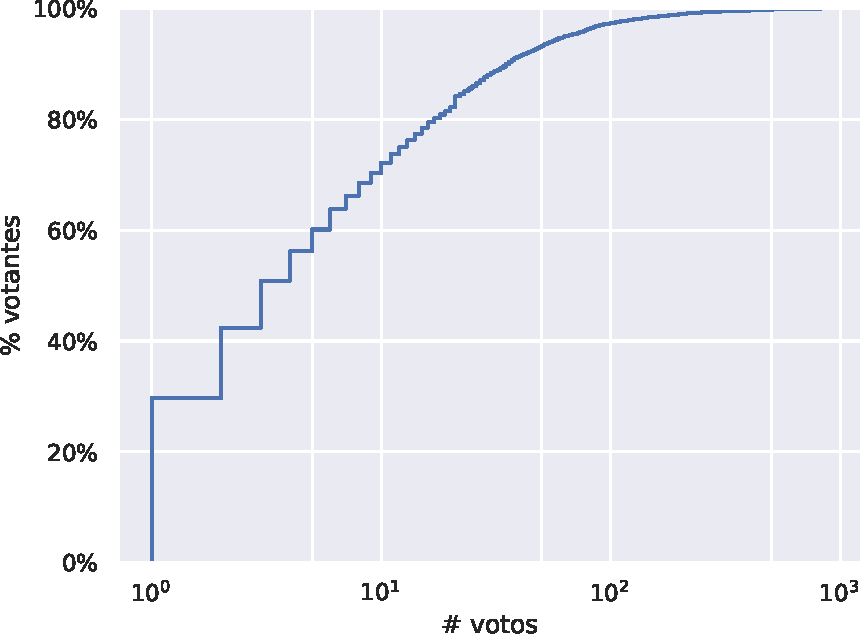
\includegraphics[width=\linewidth]{figures/04_exploracion/04_hybrid_ecdf_voters_Decentraland.pdf}
        \caption[Función de Dist. Cum. de votos por usuario de Decentraland.]{Función de Distribución Cumulativa de votos por usuario de Decentraland.}
        \label{fig:04-ecdf-voters}
    \end{minipage}\hfill\begin{minipage}{.48\linewidth}
        \centering
        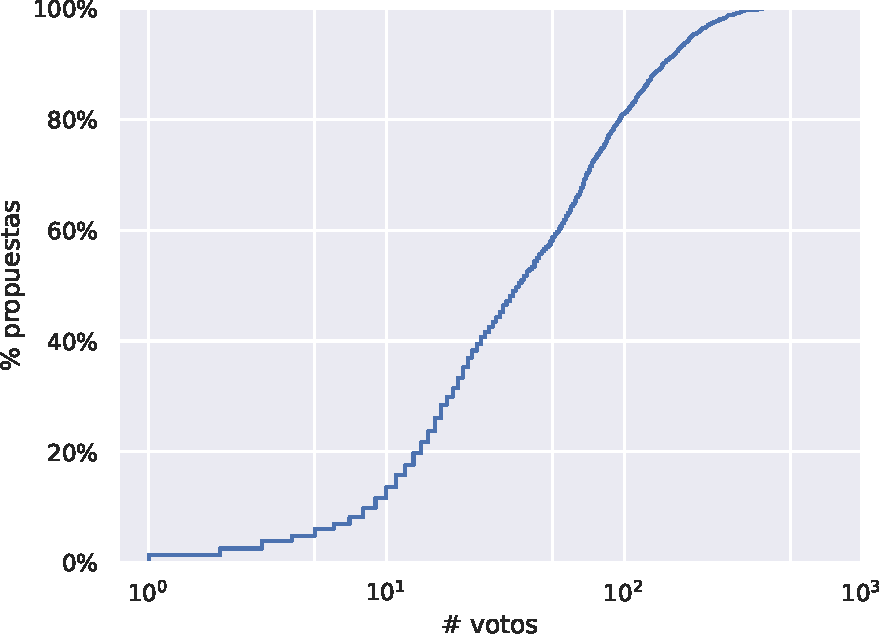
\includegraphics[width=\linewidth]{figures/04_exploracion/04_hybrid_ecdf_proposals_Decentraland.pdf}
        \caption[Función de Dist. Cum. de votos por propuesta de Decentraland.]{Función de Distribución Cumulativa de votos por propuesta de Decentraland.}
        \label{fig:04-ecdg-proposals}
    \end{minipage}
\end{figure}

Su proceso de votación está desplegado en Snapshot, donde se han presentado más de 2~000 propuestas y participan más de 7~000 votantes, emitiendo más de 115~000 votos en total. Sin embargo, como en la mayoría de las \glspl{dao}, la participación es baja, con la mayoría de los miembros votando como mucho en 3 propuestas. Aunque existen 197 miembros (${\sim}2.71\%$) que han emitido más de 100 votos cada uno, la distribución de votos en propuestas de la figura~\ref{fig:04-ecdf-voters} muestra una gran cantidad de usuarios con menos de 10 votos y una pequeña minoría con más de 100.

En cuanto a las propuestas, el grafo es más denso, con una media de 56 votos por propuesta y más de 350 propuestas con más de 100 votos. Sin embargo, la propuesta más votada cuenta con votos de solo el 5\% del total de miembros (385 votos). La figura~\ref{fig:04-ecdg-proposals} muestra de forma detallada la distribución de votos por propuesta en la organización.

% Decentraland ha experimentado un crecimiento gradual en el número de usuarios a lo largo del tiempo, como puede observarse en la figura~\ref{fig:datos-voters-tiempo} lo que plantea el desafío del arranque en frío al tratar con nuevos usuarios. Sin embargo, el problema del cold-start es aún más relevante en relación con las propuestas, pues muchos de esos miembros no volverán a participar. 
Como puede observarse en la figura~\ref{fig:datos-activos-tiempo}, el número de usuarios activos a lo largo del tiempo ha tenido picos de hasta 1~400, pero parece situarse entre los 600 y 800, con una pequeña bajada durante el verano. Además, como se observa en la figura~\ref{fig:rolling_proposals}, se crean entre 10 y 20 propuestas semanalmente, aunque en ocasiones se han observado picos de hasta 70 propuestas, lo que puede dificultar la participación.

La distribución de las propuestas creadas a lo largo de la semana es monotónica y descendente como puede verse en la figura~\ref{fig:04-propuestas-semana}, con casi el doble de propuestas creadas un lunes que en un día de fin de semana.

\begin{figure}[t]
    % \begin{minipage}[t]{.48\linewidth}
    %     \centering
    %     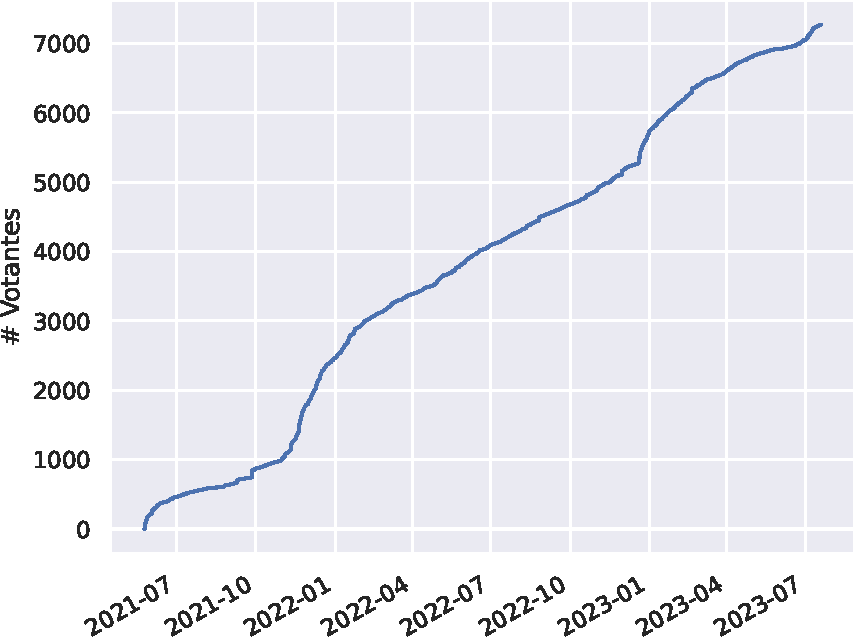
\includegraphics[width=\linewidth]{figures/04_exploracion/04_hybrid_cumcnt_users_Decentraland.pdf}
    %     \caption{Número de usuarios en Decentraland a lo largo del tiempo.}
    %     \label{fig:datos-voters-tiempo}
    % \end{minipage}\hfill%
    \begin{minipage}[t]{.48\linewidth}
        \centering
        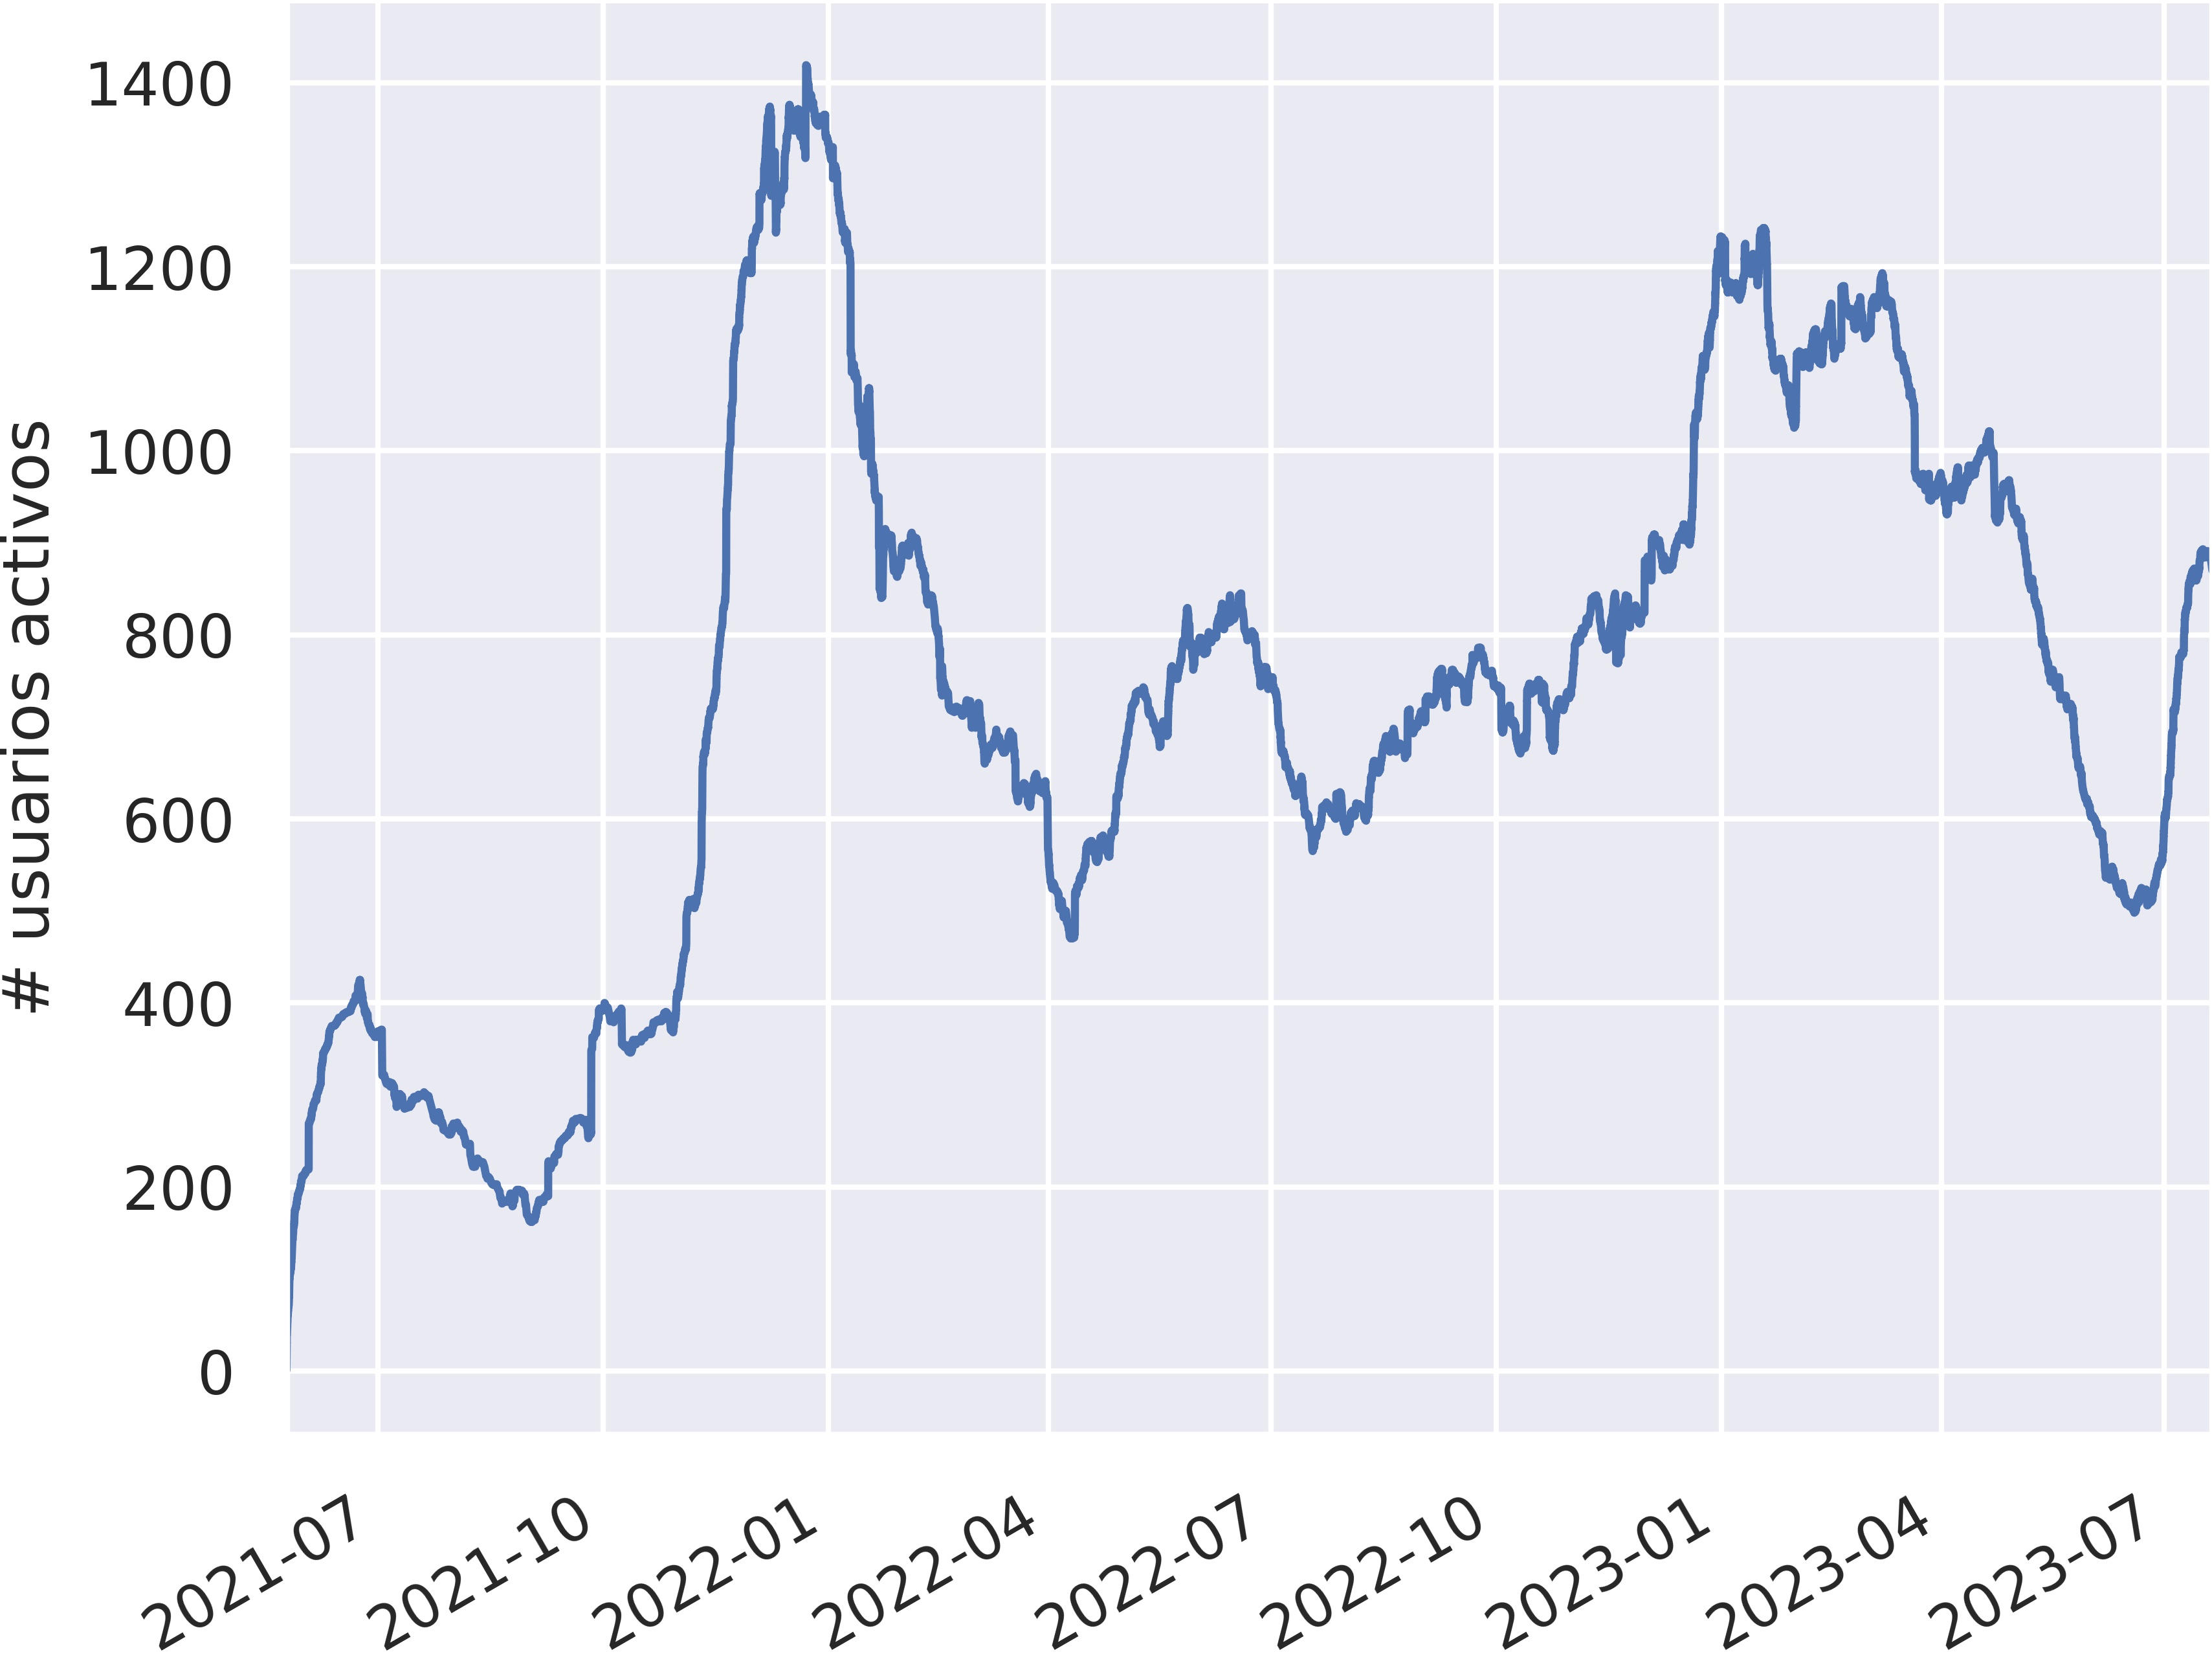
\includegraphics[width=\linewidth]{figures/04_exploracion/04c_rolling_voters_30D_Decentraland.png}
        \caption[Número de usuarios activos en Decentraland a lo largo del tiempo.]{Número de usuarios activos en Decentraland a lo largo del tiempo. Un usuario se considera activo si ha realizado un voto en una propuesta en los últimos 30 días.}
        \label{fig:datos-activos-tiempo}
    \end{minipage}\hfill%
    \begin{minipage}[t]{.48\linewidth}
        \centering
        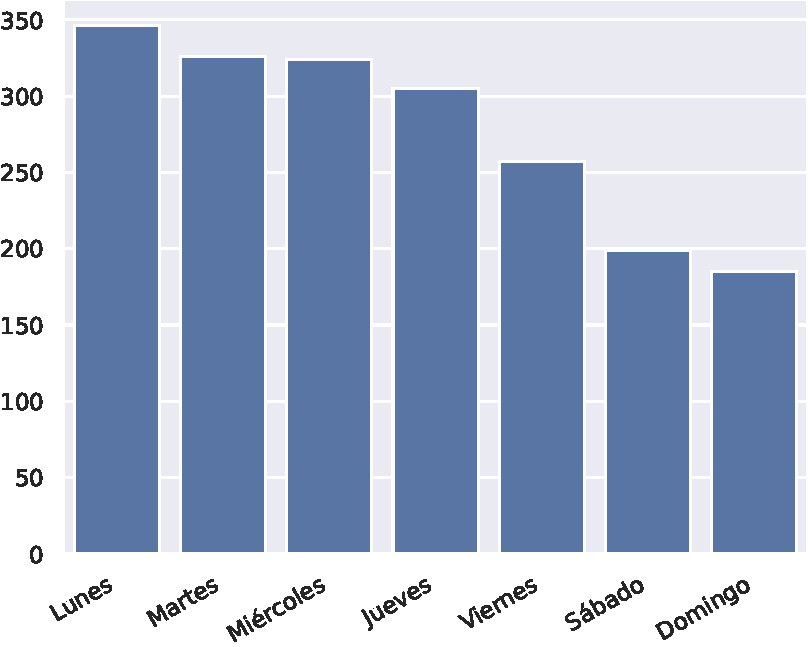
\includegraphics[width=\linewidth]{figures/04_exploracion/04_creation_dow_Decentraland.pdf}
        \caption{Número de propuestas creadas por día de la semana en Decentraland.}
        \label{fig:04-propuestas-semana}
    \end{minipage}
\end{figure}

\begin{figure}[p]
    \centering
    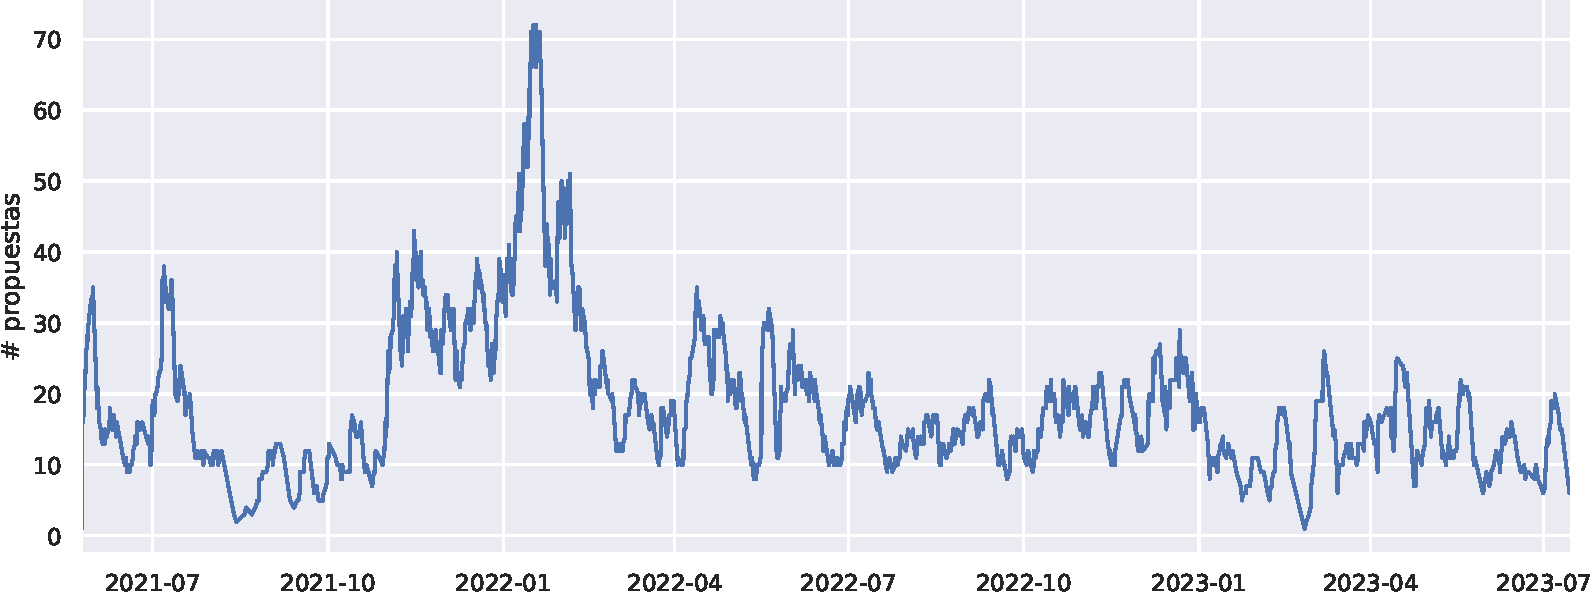
\includegraphics[width=\linewidth]{figures/04_exploracion/04c_rolling_proposals_7D_Decentraland.pdf}
    \caption[Propuestas abiertas en los últimos 7 días en la DAO Decentraland.]{Suma móvil de propuestas abiertas en los últimos 7 días en la \gls{dao} Decentraland.}
    \label{fig:rolling_proposals}
\end{figure}

% \begin{itemize}
    % \item Decentraland es una plataforma de metaverso donde los usuarios pueden comprar parcelas virtuales como \glspl{nft} utilizando criptomonedas basadas en Ethereum. Su desarrollo comenzó en 2015, en 2017 consiguió 26 millones de dólares en su \gls{ico} en la que fue lanzada al público~\cite{higgins_26_2017}, y en 2022 se valoró la plataforma con un valor de 1.2 mil millones de dólares~\cite{tangermann_12_2022}. Ha atraído la atención de grandes marcas como Samsung, Tommy Hilfiger o PricewaterhouseCoopers~\cite{noauthor_decentraland_nodate}, que han comprado \textquote{propiedades} en su mundo, y por lo tanto son miembros con pleno derecho a voto.
    % \item Su mecanismo de organización y votación está desplegado en Snapshot con más de 2~000 propuestas y 7~000 votantes, que han efectuado más de 115~000 votos.
    % \item Sin embargo, como en todas las DAOs, la participación es muy baja. La mayoría de los miembros han efectuado solo 3 votos, pero hay 197 miembros (2.71\%) que han emitido más de 100 votos cada uno, dando una media de 16 votos por votante. En la figura~\ref{fig:04-ecdf-voters} se muestra la distribución cumulativa de votos en propuestas, donde se puede ver que hay una gran mayoría de usuarios con menos de 10 votos, y una pequeña minoría con menos de 100.
    % \item Desde el punto de vista de las propuestas, el grafo es mucho más denso, con una media de 56 votos por propuesta, y hay 367 propuestas con más de 100 votos. Sin embargo, la propuesta con más votos tiene tan solo 385 votos, un 5\% del total de miembros.
    % \item En el caso de Decentraland, se han ido añadiendo usuarios poco a poco a lo largo del tiempo de vida de la organización, por lo que habrá que lidiar con el problema de cold-start con los usuarios, como se ve en la figura~\ref{fig:datos-voters-tiempo}
    % \item Normalmente se generan entre 10 y 20 propuestas a la semana, una cantidad que puede parecer manejable en un principio. Sin embargo, hay épocas en las que se crean 30 propuestas a la semana, y picos de hasta 70, como se puede ver en la figura~\ref{fig:rolling_proposlas}.
    % \item En general los usuarios votan cualquier día de la semana por igual, con menos votos realizados en Domingo. Sin embargo, las propuestas si que forman una distribución de campana con un pico de propuestas creadas en Martes, y muchas menos propuestas creadas de Viernes a Domingo. En general, los usuarios votan en los primeros 2 días de creación de la propuesta, a pesar de que tienen un tiempo de votación de 7 días.
% \end{itemize}

\begin{figure}[p]
    \centering
    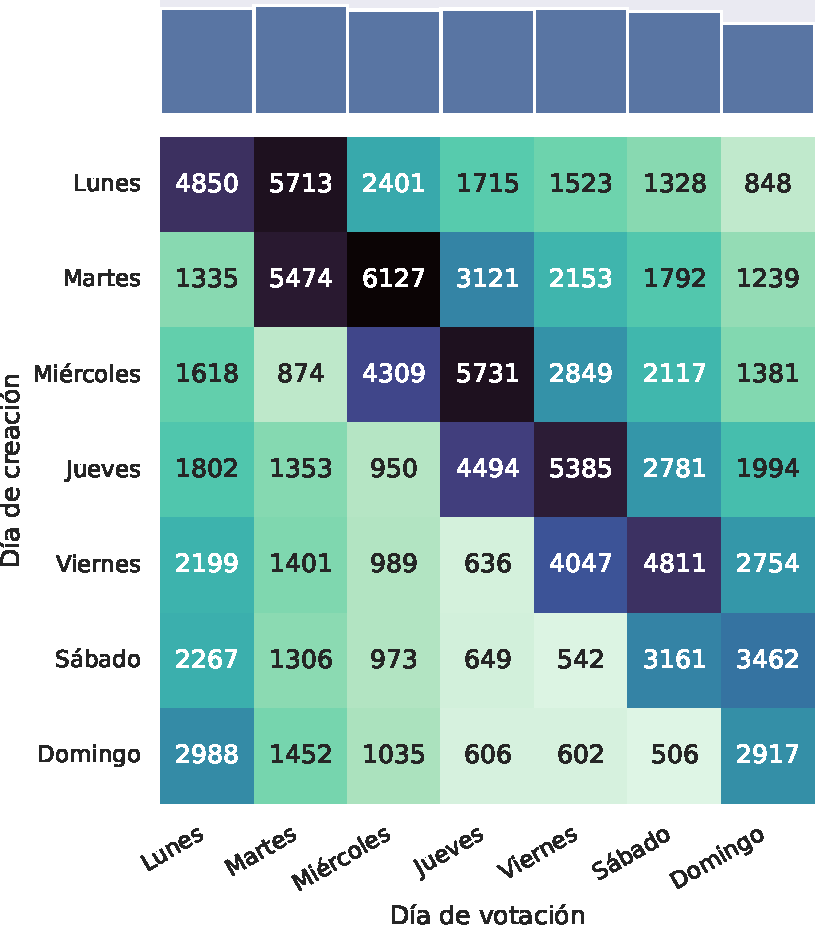
\includegraphics[scale=.8]{figures/04_exploracion/04c_heatmap_proposals_Decentraland.pdf}
    \caption[Mapa de calor día de voto y fecha de creación propuesta.]{Mapa de calor con distribución marginal ilustrando la correlación entre el día en el que se produce un voto y el día de creación de la propuesta en la que se realizó el voto.}
    \label{fig:heatmap-propuestas}
\end{figure}

En las distribuciones marginales de la figura~\ref{fig:heatmap-propuestas}, se pueden observar patrones interesantes en la distribución de los votos y la creación de propuestas en Decentraland a lo largo de los días de la semana. Sobre las votaciones, los usuarios muestran una tendencia uniforme a lo largo de la semana, con una ligera bajada de participación los sábados y domingos, y un ligero repunte los martes, prefiriendo los usuarios la actividad en los días hábiles. % Por otro lado, la distribución de la creación de propuestas es más heterogénea, siguiendo una distribución con una notable campana cuyo máximo es el martes, y una disminución gradual a lo largo de la semana con una marcada reducción de propuestas durante el fin de semana, desde el viernes hasta el domingo.

En la sección central de la figura, se presenta un mapa de calor que ilustra la cantidad de propuestas y votos emitidos cada día de la semana. Se observa que las propuestas reciben la mayor cantidad de votos al día siguiente de su creación, y, a medida que transcurren los días, experimentan una disminución en la cantidad de votos recibidos. Esta regla sólo se rompe los lunes, que puede haber más votos que en Domingo para las propuestas creadas ese día, ya que la participación es menor como se indica en el párrafo anterior.

\section{Propuesta de sistema}

% \begin{itemize}
    % \item Se buscarán modelos probados ya implementados en librerías, uno basado en contenido y otro basado en las relaciones, para realizar las recomendaciones.
    % \item El modelo basado en contenido tendrá sólo en cuenta el título y la descripción de las propuestas, utilizando modelos de \gls{pln}.
    % \item El modelo basado en filtrado colaborativo estará basado en \gls{gnn}, pensando en la expansión del grafo de relaciones más allá de la \gls{dao} en un posible trabajo futuro.
    % \item Se creará un sistema híbrido que combine ambos modelos.
    % \item No se tendrá en cuenta más contexto en ninguno de los dos sistemas. Ninguno de los dos tendrá en cuenta el contexto temporal, pero se les añadirá un pos-filtrado para evitar recomendar propuestas que ya estén cerradas.
    % \item Sin embargo, la evaluación si que tendrá que ser dividiendo los folds en el tiempo, y teniendo en cuenta dicha característica al reportar las métricas.
    % \item Asumiremos que el sistema recomendador se ejecutará periódicamente (por ejemplo, cada semana o cada día), y se evaluará de manera acorde. No se ejecutará de manera continua. Asumimos que el modelo puede ser re-entrenado por completo cada vez que se quieran realizar nuevas recomendaciones.
    % \item Por esa razón, el entrenamiento de los sistemas desarrollados deberían ser rápidos (de varios minutos, como mucho).
% \end{itemize}

En esta sección se realiza una propuesta inicial del posible \gls{sr}. Se buscará utilizar modelos de \glspl{sr} ya validados y disponibles en librerías estándar. Se construirán tres modelos: uno siguiendo un enfoque basado en contenido, otro siguiendo un enfoque basado en \gls{cf}, y un tercero que será un híbrido que combine los otros dos sistemas.

El modelo basado en contenido se limitará a analizar únicamente el título y la descripción de las propuestas, empleando técnicas de \gls{pln}. Por otro lado, el modelo basado en filtrado colaborativo se basará en analizar el grafo bipartito formado por los votantes y las propuestas, utilizando una \gls{gnn}. El sistema híbrido integrará los \textit{rankings} producidos por los dos otros sistemas.

En ninguno de los dos sistemas propuestos se considerará más contexto ni información adicional como el tiempo o día de creación de la propuesta. No obstante, se aplicará un pos-filtrado para evitar recomendar aquellas propuestas cuyo periodo de votación haya concluido. Para ello, el método encargado de realizar las $k$ recomendaciones utilizando el modelo recibirá el conjunto de propuestas consideradas \textit{recomendables}, y se encargará de clasificarlas según su idoneidad, y devolviendo las $k$ mejores recomendaciones para cada usuario.

De esta manera, el modelo se ejecutará en intervalos discretos de tiempo, y la evaluación será en consecuencia. Es decir, asumiendo que el recomendador se ejecutará de forma periódica (por ejemplo, cada semana o cada día) y se evaluará de acuerdo con esta periodicidad. Por ejemplo, para poder enviar un boletín o \textit{newsletter} personalizado con dicha periodicidad y mejorar la participación~\cite{maslowska_effectiveness_2011}. No se contempla la ejecución continua, sino que presupone la posibilidad de reentrenar completamente el modelo en cada ocasión que se desee realizar nuevas recomendaciones. Por consiguiente, uno de los requisitos es que el entrenamiento de los sistemas desarrollados sea rápido, con tiempos de entrenamiento en el orden de minutos.

\chapter{Entrenamiento y validación de los sistemas}
\label{chap:entrenamiento_y_validacion}

\nocite{aggarwal_recommender_2016}

% \begin{itemize}
%     \item En sistemas recomendadores, podemos distinguir dos paradigmas de evaluación~\cite{aggarwal_recommender_2016}:
%     \begin{itemize}
%         \item La evaluación online, en la que usuarios interactuan directamente con el \gls{sr} y se evalua como interactúan los usuarios con las recomendaciones presentadas
%         \item La evaluación offline con datos históricos, en la que se entrena un modelo utilizando interacciones previas de los usuarios (y tal vez otra información contextual).
%         \item La ventaja de usar un dataset offline es que se pueden comparar varios sistemas recomendadores, pero no conocemos como se comportarán en la realidad ni si se adaptarán a los cambios del conjunto de datos.
%         \item Obviamente, nuestro caso se tratará de una evaluación offline pues usamos datos históricos.
%         \item De todas formas, no podríamos hacer evaluación online utilizando solamente datos de la blockchain o las APIs públicas, necesitaríamos integrar el sistema en la plataforma.
%     \end{itemize}
%     \item Además, debido a la característica de los datos (cap~\ref{chap:problema}) no hay mucho escrito y ha habido que inventarse técnicas.
%     \item El objetivo es poder usar métricas clásicas de recsys como precision, ndcg o map, pero dividiendo los folds de manera temporal.
%     \item Por simplificar, asumimos que el tiempo es discreto, y que los modelos se entrenan periódicamente. Por ejemplo, cada día o cada semana, como se explica más en profundidad en el capítulo~\ref{chap:problema}.
%     \item En la siguiente sección se explorará como se ha realizado la división de los datos.
% \end{itemize}

En el ámbito de los sistemas recomendadores, existen dos paradigmas principales de evaluación~\cite{aggarwal_recommender_2016}. Por un lado, la \textit{evaluación online} utiliza la interacción directa de los usuarios con el sistema recomendador ya desplegado, permitiendo evaluar cómo responden los usuarios a las recomendaciones presentadas en tiempo real. Por otro lado, la \textit{evaluación offline} se basa en el uso de datos históricos, donde se entrena un modelo utilizando las interacciones previas de los usuarios, junto con cualquier información contextual disponible.

La ventaja de utilizar un dataset offline radica en la posibilidad de comparar varios sistemas recomendadores bajo condiciones controladas, aunque también sería posible utilizar A/B testing en una evaluación online para probar distintos modelos, asignando modelos distintos a cada usuario. Sin embargo, es importante tener en cuenta que el enfoque offline no proporciona una visión completa de cómo se comportarán los sistemas en la realidad ni si serán capaces de adaptarse a los cambios en el conjunto de datos a lo largo del tiempo. En nuestro caso, debido a la disponibilidad de datos históricos, utilizaremos una evaluación offline para entrenar y validar nuestros sistemas recomendadores, pero añadiendo la variable temporal para hacer más robusta la validación de los modelos y evitar el \textit{data leakage}, un riesgo presente en la evaluación offline de sistemas recomendadores~\cite{ji_critical_2023}.

La realización de una evaluación online requeriría una integración más estrecha del sistema recomendador desarrollado en la plataforma, lo que podría no ser factible utilizando únicamente datos de la blockchain o las APIs públicas disponibles. Sin embargo, al ser software libre, podría realizarse un fork de alguna de las plataformas modificando su interfaz para añadir el sistema recomendador, o crear una extensión de navegador que efectúe las recomendaciones.

Además, debido a las características específicas de estos datos, como se detalla en el capítulo~\ref{ch:planteamiento-problema}, se ha tenido que desarrollar técnicas y enfoques adaptados a nuestro contexto, que tengan en cuenta que las propuestas están abiertas durante un tiempo limitado. El objetivo es emplear métricas clásicas de sistemas recomendadores, como precisión, \acrshort{ndcg} o \acrshort{map} para que sean más fácilmente interpretables, pero teniendo en cuenta la naturaleza temporal de nuestros datos.

\section{División del conjunto de datos}
\label{sec:division_datos}

% \begin{itemize}
    % \item Debido a que no hay nada escrito sobre recomendadores de ítems acotados en el tiempo, no hay nada estándar o extendido sobre como evaluarlos.
    % \item La idea es segmentar el dataset en dos conjuntos, uno para entrenamiento, y otro para evaluación. Además, queremos validar el modelo con varios conjuntos de datos, por lo que realizaremos una especie de validación cruzada, pero utilizando el timestamp de los votos.
    % \item En un principio, podríamos usar la clase \url{TimeSeriesSplit} de Scikit-learn~\cite{pedregosa_scikit-learn_2011}, en la que se divide el conjunto de datos en K intervalos con el mismo número de muestras, pero los datos se ordenan por un timestamp, y se cogen incrementalmente. Es decir, el segundo fold incluye para entrenamiento los folds del primero, y el tercero incluye los de los dos anteriores, etc.
    % \item En nuestro caso, en lugar de dividir en intervalos con el mismo número de muestras, como la distribución de actividad no es uniforme en el tiempo (véase la figura~\ref{fig:rolling_proposals}), dividimos de tal manera que el intervalo temporal siempre sea el mismo, por ejemplo 7 días.
    % \item De esta manera, el primer fold cuenta de entrenamiento con los datos de la primera semana, y testea con la segunda. El segundo cuenta con los datos de las dos primeras semanas y testea con la tercera, y así...
    % \item Además, casi todas las propuestas del conjunto de entrenamiento ya han sido cerradas, y no pueden ser recomendadas, por lo tanto, no tiene sentido calcular las métricas de evaluación en train.
    % \item De igual modo, no tiene sentido usar todas las interacciones de test, pues muchas propuestas aún no han sido creadas, no pueden tener votos, y no hay ninguna interacción que sirva para el entrenamiento.
%     \item Por esa razón, las métricas se calculan únicamente sobre las interacciones producidas en el conjunto de test en propuestas que ya estaban creadas en el intervalo de train. Es decir, el conjunto de test es filtrado para mantener solo las interacciones en propuestas ya creadas. La figura~\ref{fig:example-train-test} ilustra con un ejemplo este comportamiento.
%     \item Tras desarrollar este sistema, descubrí que \textcite{macedo_context-aware_2015} ya habían realizado un método similar para un sistema de recomendación de eventos, con la diferencia de añadir una cota inferior al conjunto de entrenamineto, tratándose de un descubrimiento independiente o redescrubrimiento. La principal diferencia es que \citeauthor{macedo_context-aware_2015} añaden también una cota inferior al conjunto de entrenamiento.
% \end{itemize}

La evaluación de sistemas recomendadores con elementos limitados en el tiempo presenta un desafío, ya que no existe una metodología estándar ampliamente aceptada para su evaluación.

La estrategia seguida para abordar este problema es dividir el conjunto de datos en dos partes distintas: una para el entrenamiento del modelo y otra para su evaluación. Sin embargo, dado que se busca validar el modelo con múltiples subconjuntos de datos, se implementará una variante de la validación cruzada temporal. En este enfoque, se utilizarán las marcas de tiempo asociadas a los votos para realizar una partición temporal del conjunto de datos.

Inicialmente, consideramos utilizar la clase \url{TimeSeriesSplit} de Scikit-learn~\cite{pedregosa_scikit-learn_2011} para la división del conjunto de datos. Esta clase ordena los datos por su marca temporal, y divide el conjunto en $K$ intervalos, cada uno con un número igual de muestras. Además, las particiones son incrementales, de tal manera que en la partición $k$-ésima se retorna el split $k+1$ como conjunto de test, pero todos los splits de 0 a $k$ para entrenamiento, siendo cada uno un superconjunto del anterior.

Sin embargo, en nuestro caso, la distribución de actividad no es uniforme en el tiempo, como se ilustra en la figura~\ref{fig:rolling_proposals}. Por lo tanto, optamos por una estrategia alternativa, en la que el número de elementos en cada fold no es necesariamente el mismo, pero el intervalo de tiempo entre particiones sí lo es, y manteniendo que cada conjunto de entrenamiento sea un superconjunto del anterior. De hecho, podemos identificar cada fold por la marca de tiempo que divide los dos conjuntos. Los votos realizados antes de ese momento $t$ pertenecerán a entrenamiento y los realizados posteriormente, a la evaluación, lo que en el campo de \textit{forecasting} se conoce como \textit{out-of-sample testing}~\cite{tashman_out--sample_2000}.

\begin{figure}[b!]
    \centering
    % \fbox{\parbox{.7\linewidth}{Aquí va una figura creada con \url{draw.io} en la que se muestre como se divide el conjunto de datos en train y test, dado un timsetamp. Las propuestas serán rectángulos alargados, que tendrán puntos de colores que simbolizarán el feedback. Los puntos de un color estarán en el conjunto de entrenamiento, y los puntos de otro color estarán en test. También habrá puntos en blanco que no estén en ninguno de los dos conjuntos. Debe haber mínimo: (i) una propuesta con feedback en train y en test (ii) una propuesta que pase un poco a test pero sin feedback, (iii) una propuesta que no salga de train pero con puntitos de train, (iv) una propuesta solo en test, con puntitos en blanco porque no estan en ninguno de los dos conjuntos.}}
    % 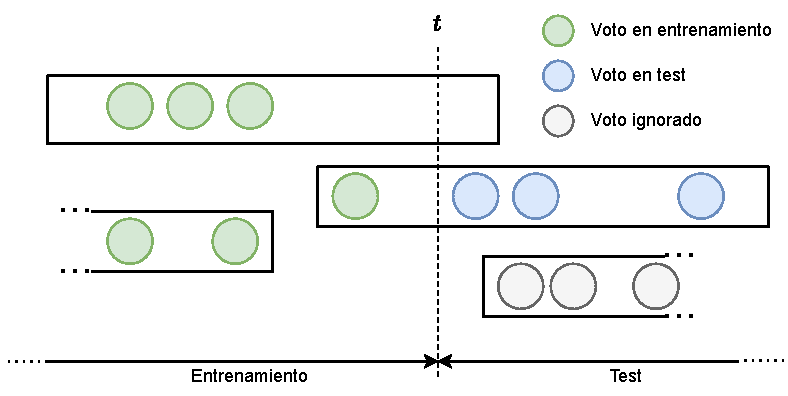
\includegraphics{figures/04_validacion/rs-time-folds-evaluacion.drawio.pdf}
    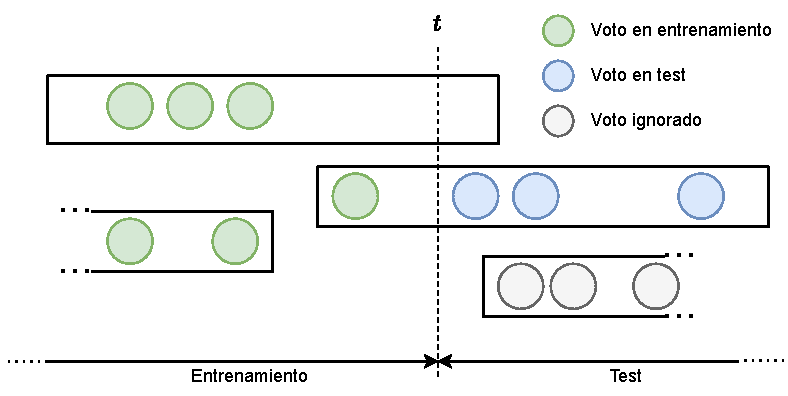
\includegraphics{figures/04_validacion/rs-time-folds-evaluacion.drawio.pdf}
    \caption[Esquema de la división en particiones de train y test.]{Esquema ejemplificando la creación de particiones de entrenamiento y test.}
    \label{fig:example-train-test}
\end{figure}

Además, es importante destacar que en el conjunto de entrenamiento, la mayoría de las propuestas ya han sido cerradas y, por lo tanto, no pueden ser objeto de recomendación pues los usuarios no podrían votar en ellas, aunque son útiles para crear el modelo del usuario.

De manera similar, al considerar el conjunto de prueba, nos encontramos con que muchas propuestas aún no han sido creadas y, como resultado, no habrán podido ser votadas por los usuarios durante el conjunto de entrenamiento y una predicción realizada sobre esas propuestas usando filtrado colaborativo carecerá de validez.
% Sin embargo, al tratarse de un problema de ranking, sí que se intentará recomendar esas propuestas que sólo aparecen en test. 
El recomendador basado en contenido sí que podrá realizar recomendaciones satisfactorias, mientras que el basado en filtrado colaborativo les asignará una prioridad mínima y probablemente no sean recomendadas. % Nótese que aunque sí podrían ser recomendadas basándose en el contexto y el contenido aunque no tengan aún votos, se ha decidido utilizar el mismo método de evaluación para los dos sistemas recomendadores desarrollados.

Por esa razón, las métricas se calculan exclusivamente utilizando las interacciones generadas en el conjunto de prueba en propuestas que ya estaban creadas durante el intervalo de entrenamiento. Es decir, el conjunto de prueba se filtra para conservar únicamente las interacciones en propuestas abiertas. La figura~\ref{fig:example-train-test} ejemplifica este procedimiento.

Tras desarrollar este sistema, se descubrió que~\textcite{macedo_context-aware_2015} ya habían implementado un método similar para un sistema de recomendación de eventos, aunque con la distinción de agregar un límite inferior al conjunto de entrenamiento. % Este hallazgo constituye un descubrimiento independiente o redescubrimiento.

Se ha implementado un código en Python para llevar a cabo este proceso, utilizando la tabla que contiene los votos y la que contiene las marcas de tiempo de las propuestas. Este código se encuentra en la función \url{timeFreqSplitCurrent}, ubicada en el módulo \url{src.model_selection}. Este módulo está disponible en el repositorio del proyecto en GitHub~\cite{davo_daviddavoupm-tfm-notebooks_2024}. Además, se incluye una versión simplificada del código en esta memoria, que se puede encontrar en Código~\ref{cod:timeFreqSplitCurrent}.

\begin{code}
%  \begin{minted}[breaklines]{python}
\begin{lstlisting}[language=Python]
def timeFreqSplit(dfv: pd.DataFrame, freq: str, dfp: pd.DataFrame, normalize=True):
  times = pd.date_range(dfv['timestamp'].min(), dfv['timestamp'].max(), 
                        freq=freq, normalize=normalize)
  for train_end in times[:-1]:
    train = df[df[timestamp_col] <= train_end]
    test = df[ (train_end < df['timestamp'])]
    
    open_proposals = dfp[ (dfp['start'] < train_end) & (train_end < dfp['end']) ]['id']
    test_filtered = test[test['itemID'].isin(open_proposals)]

    yield train, test_filtered
\end{lstlisting}
\caption{Simplificación del método \url{timeFreqSplit} del módulo \url{src.model_selection}}
\label{cod:timeFreqSplitCurrent}
\end{code}

Finalmente, para acomodar los datos al modelo LightGCN de Microsoft que necesita que los usuarios en test hayan estado previamente presentes en entrenamiento, se ignoran los votos de los usuarios nuevos: aquellos que aparecen tan sólo en el conjunto de test.

\subsection{Exploración de la división en folds de los datos de Decentraland}
\label{subsec:exploracion-folds}

% \begin{itemize}
%     \item En nuestro caso, para crear un sistema recomendador para Decentraland, se ha decidido dividir los folds en 7 días, debido a que es el tiempo de duración de las propuestas. Como contamos con datos de 2 años desde Mayo 2021 hasta Julio 2023, contamos con 112 folds con los que poder probar el sistema. En la figura~\ref{fig:04-first-ten-folds} se muestra el número de datos en entrenamiento y test de los 10 primeros folds.
%     \item Debido a restricciones computacionales, utilizamos solo los 10 últimos folds, con datos desde mayo hasta julio de 2023. Estos folds tienen entre 106~000 y 115~000 votos para el conjunto de entrenamiento (recordemos que son incrementales), y entre 13 y 25 propuestas en el conjunto de test, con una media de 381 votos de 123 usuarios con los que probar el modelo.
%     \item En un sistema de filtrado colaborativo, es necesario que las propuestas que vamos a recomendar tengan ya ciertos votos, pues, además de toda la historia incremental de votaciones que nos sirve para entrenar el modelo del usuario, es necesario saber qué tipos de usuarios han votado en una propuesta para recomendarla. En estos 10 folds, hay una media de 1283 votos por 325 usuarios en las propuestas que están abiertas en el momento de realizar el split y van a aparecer en la evaluación.
%     \item La tabla~\ref{tab:open_proposals} muestra más en profundidad los datos de cada uno de los 10 folds.
% \end{itemize}

Para desarrollar un sistema recomendador con los datos de la organización Decentraland, se ha optado por dividir los datos en folds de 7 días cada uno, pues es el período típico de duración de las propuestas dentro de la plataforma. Con los datos recopilados desde mayo 2021 hasta julio de 2023, se generan un total de 112 folds que podrían utilizarse para la evaluación del sistema. El conjunto de entrenamiento en estos folds es incremental, como se muestra en la figura~\ref{fig:04-first-ten-folds}.

\begin{figure}
    % No hace falta actualizarla porque en los primeros folds todas las propuestas eran de 7 días
    \centering
    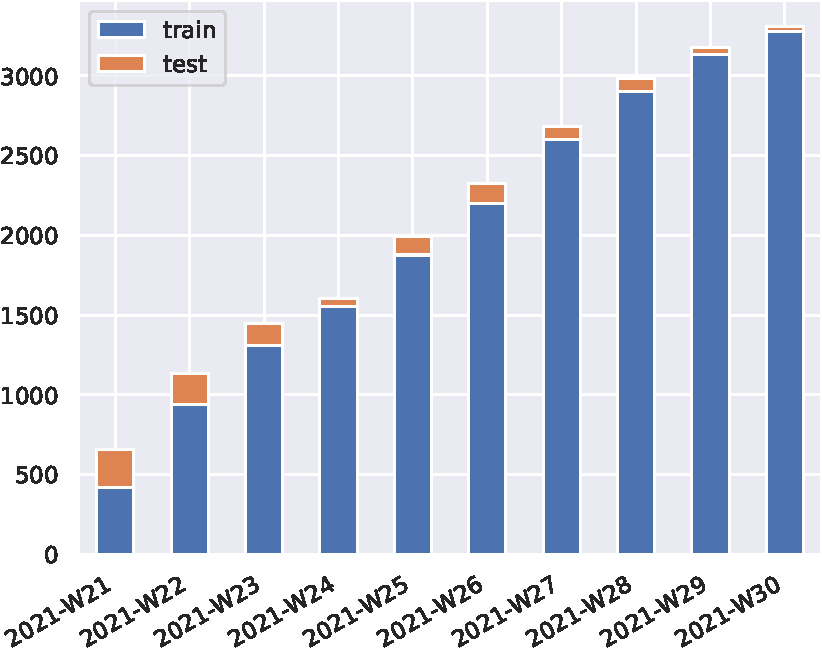
\includegraphics[width=.6\linewidth]{figures/04_validacion/10_first_folds_W-THU_True_Decentraland.pdf}
    \caption{Cantidad de votos en entrenamiento y prueba de los primeros 10 folds de la organización Decentraland.}
    \label{fig:04-first-ten-folds}
\end{figure}

% Source: 20_results.ipynb [9]
% Actualizado 2024-03-23
Sin embargo, por restricciones computacionales, se ha limitado el análisis a los 10 últimos folds, que abarcan desde mayo hasta julio de 2023. Estos folds contienen en entrenamiento casi todos los votos disponibles, yendo desde 106~000 a 115~000 votos. Por otro lado, el conjunto de test contiene una media de 439 votos de 142 usuarios realizados en entre 13 y 25 propuestas.

% No es necesario actualizar esto pues es en train
En un sistema de filtrado colaborativo, es fundamental que las propuestas a recomendar ya cuenten con cierta cantidad de votos para poder evaluarlas. Estas propuestas están abiertas en el momento de realizar el split, y aparecerán también en la evaluación. En estos 10 folds, hay una media de 1283 votos por 325 usuarios en dichas propuestas.

\begin{table}
    % Source: 20_results.ipynb [8]
    % Actualizado 2024-03-23
    \centering\footnotesize
    \begin{tabular}{l|r|rrrr|rrrr}
    \toprule
    \multicolumn{1}{c|}{\multirow{2}{*}{Semana}} &
    \multirow{2}{*}{\shortstack{Prop.\\ abiertas}} &
    \multicolumn{4}{c|}{\textbf{Solo entrenamiento}} &
    \multicolumn{4}{c}{\textbf{Solo validación}} \\
    \multicolumn{1}{c|}{} & & Votos & Usuarios & vpp & vpu & Votos & Usuarios & vpp & vpv \\
    \midrule
% 2023-W19 & 18 & 1627 & 358 & 90.39 & 4.54 & 322 & 130 & 17.89 & 2.48 \\
% 2023-W20 & 25 & 1346 & 305 & 53.84 & 4.41 & 713 & 147 & 28.52 & 4.85 \\
% 2023-W21 & 19 & 1483 & 305 & 78.05 & 4.86 & 296 & 108 & 15.58 & 2.74 \\
% 2023-W22 & 13 & 819 & 247 & 63.00 & 3.32 & 267 & 89 & 20.54 & 3.00 \\
% 2023-W23 & 13 & 631 & 191 & 48.54 & 3.30 & 291 & 94 & 22.38 & 3.10 \\
% 2023-W24 & 16 & 872 & 225 & 54.50 & 3.88 & 326 & 110 & 20.38 & 2.96 \\
% 2023-W25 & 17 & 1136 & 278 & 66.82 & 4.09 & 331 & 127 & 19.47 & 2.61 \\
% 2023-W26 & 10 & 838 & 278 & 83.80 & 3.01 & 204 & 92 & 20.40 & 2.22 \\
% 2023-W27 & 21 & 1591 & 469 & 75.76 & 3.39 & 683 & 198 & 32.52 & 3.45 \\
% 2023-W28 & 23 & 2493 & 600 & 108.39 & 4.16 & 382 & 141 & 16.61 & 2.71 \\
2023-W19 & 18 & 1627 & 358 & 90.39 & 4.54 & 354 & 139 & 19.67 & 2.55 \\
2023-W20 & 25 & 1346 & 305 & 53.84 & 4.41 & 811 & 169 & 32.44 & 4.80 \\
2023-W21 & 19 & 1483 & 305 & 78.05 & 4.86 & 332 & 122 & 17.47 & 2.72 \\
2023-W22 & 13 & 819 & 247 & 63.00 & 3.32 & 289 & 101 & 22.23 & 2.86 \\
2023-W23 & 13 & 631 & 191 & 48.54 & 3.30 & 341 & 118 & 26.23 & 2.89 \\
2023-W24 & 16 & 872 & 225 & 54.50 & 3.88 & 391 & 132 & 24.44 & 2.96 \\
2023-W25 & 17 & 1136 & 278 & 66.82 & 4.09 & 360 & 148 & 21.18 & 2.43 \\
2023-W26 & 10 & 838 & 278 & 83.80 & 3.01 & 239 & 107 & 23.90 & 2.23 \\
2023-W27 & 21 & 1591 & 469 & 75.76 & 3.39 & 890 & 249 & 42.38 & 3.57 \\
2023-W28 & 23 & 2493 & 600 & 108.39 & 4.16 & 384 & 142 & 16.70 & 2.70 \\
    \bottomrule
    \end{tabular}
    \caption{Número de propuestas abiertas en cada uno de los folds durante las últimas 10 semanas en Decentraland. Bajo \textit{Solo entrenamiento} se muestra el número de votos emitidos en esas propuestas que se han usado dentro del conjunto de entrenamiento, y los usuarios que han emitido esos votos. Un usuario puede haber votado en varias propuestas. A la derecha, bajo \textit{Solo validación} se muestra el número de votos emitidos en las propuestas durante la fase de validación. \textit{vpp} es el ratio de Votos Por Propuesta, y \textit{vpv} es el ratio de votos por Votante.}
    \label{tab:open_proposals}
\end{table}

En la tabla~\ref{tab:open_proposals} se muestra más en profundidad los datos de cada uno de los 10 folds, pero hay que destacar que los votos por cada votante en validación son en general muy bajos, a penas superando los 3 \gls{vpv} en dos de los folds.

% \begin{figure}
%     \centering
%     % \includegraphics{}
%     % \fbox{\parbox{.7\linewidth}{Aquí va un gráfico de barras que tiene en el eje X el fold actual, y en el eje Y el número de propuestas abiertas. Cada color de la barra es una DAO distinta. El problema de este gráfico es que si el número de propuestas abiertas es demasiado variable, o las diferencias entre las DAOs escogidas son muy grandes, entonces no servirá de nada.}}
%     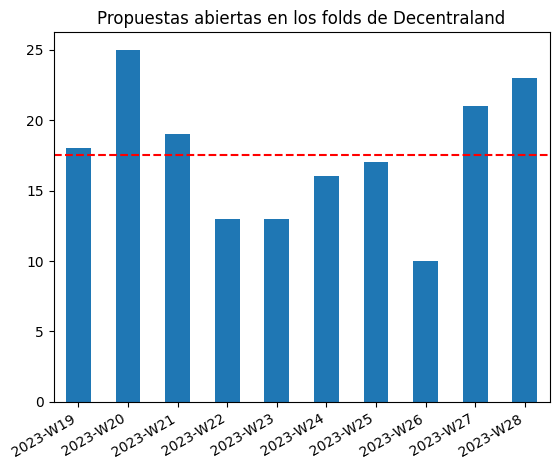
\includegraphics[width=10cm]{figures/04_validacion/propuestas_abiertas_decentraland.png}
%     \caption[Número de propuestas abiertas durante las últimas 10 semanas en Decentraland.]{Número de propuestas abiertas durante las últimas 10 semanas en Decentraland. Hubo una media (en rojo) de $17.5\pm4.72$ propuestas con las que verificar el modelo.}
%     \label{fig:open_proposals}
% \end{figure}

\section{Métricas utilizadas}
\label{subsec:metricas}

En esta sección se presentan métricas offline comúnmente empleadas en el ámbito de la recuperación de información y sistemas recomendadores. Se han utilizado las métricas disponibles en la librería Microsoft Recommenders~\cite{argyriou_microsoft_2020}.

\subsection{Precisión y exhaustividad}

\newcommand{\recall}[1]{recall@#1}
\newcommand{\precision}[1]{precision@#1}

% \begin{itemize}
%     \item Son métricas populares en la evaluación de sistemas recomendadores que han saltado del campo de la recuperación de información.
%     \item La precisión puede definirse como la probabilidad de que un ítem recuperado sea relevante, es decir el ratio entre el número de ítems relevantes recuperados y el número de ítems recuperados. 
%     \item La exhaustividad o \textit{recall} se define como la probabilidad de que un ítem seleccionado sea relevante, es decir, el ratio entre el número de ítems relevantes recuperados y el número total de ítems relevantes~\cite{herlocker_evaluating_2004}.
%     \item En un sistema recomendador que efectúa un ranking de los ítems a recomendar, podemos definir estas métricas dependiendo de los top $k$ items que elijamos recomendar, llamadas por su término en inglés $precision@k$ y $recall@k$. La fórmula de estas métricas se define en las ecuaciones \ref{eq:precision_at_k, eq:recall_at_k}.
%     \item El valor de estas métricas es muy dependiente de la $k$, por lo que no se pueden comparar métricas con distinto $k$.
%     \item Además, el mayor problema de estas métricas es que si el número de elementos relevantes es menor que $k$, como en nuestro caso, incluso un oráculo perfecto tendrá un valor menor que 1~\cite{manning_chapter_2008}.
% \end{itemize}

Las métricas de precisión y exhaustividad son ampliamente utilizadas en la evaluación de sistemas recomendadores, adoptadas desde el campo de la recuperación de información. La precisión se define como la probabilidad de que un ítem recuperado sea relevante, expresada como el cociente entre el número de ítems relevantes recuperados y el número total de ítems recuperados. Por otro lado, la exhaustividad, también conocida como recall, indica la probabilidad de que un ítem seleccionado sea relevante, calculada como el cociente entre el número de ítems relevantes recuperados y el número total de ítems relevantes~\cite{herlocker_evaluating_2004}.

En el contexto de un sistema recomendador que clasifica los ítems para su recomendación, estas métricas pueden ser adaptadas para evaluar únicamente los $k$ primeros ítems recomendados, conocidas como \textit{precisión en k} ($\precision{k}$) y \textit{exhaustividad en k} ($\recall{k}$). La fórmula de estas métricas se define en las siguientes ecuaciones:

\begin{minipage}{.5\textwidth}
    \begin{equation}\label{eq:precision_at_k}
        \precision{k} = \frac{|\text{items rel. rec. en $k$}|}{k}
    \end{equation}
\end{minipage}\begin{minipage}{.5\textwidth}
    \begin{equation}\label{eq:recall_at_k}
        \recall{k} = \frac{|\text{items rel. rec. en $k$}|}{|\text{items rel. en $k$}|}
    \end{equation}
\end{minipage}

Es importante tener en cuenta que el valor de estas métricas es altamente sensible al valor de $k$, por lo que no se pueden comparar métricas con distintos valores de $k$. Además, otro importante defecto de estas métricas ocurre cuando el número de elementos relevantes es menor que $k$, ya que incluso un sistema perfecto tendría un valor menor que 1 en estas métricas~\cite{manning_chapter_2008}.

Por esa razón, se consideró usar la métrica $r-precision$, la cual tiene en cuenta el número de documentos relevantes ($R$) para una consulta y calcula la precision en $R$ ($precision@R$), adaptando el valor de $k$ al número de documentos relevantes~\cite{manning_chapter_2008}. Como $k=R=\text{items rel. en k}$, esta métrica es equivalente al $recall@R$.

Sin embargo, a pesar de su potencial utilidad, no se empleó esta métrica debido a su ausencia en la librería Microsoft Recommenders~\cite{argyriou_microsoft_2020}. Su implementación requeriría tiempo adicional y podría afectar significativamente al tiempo de ejecución de la evaluación del modelo, y sus resultados están correlacionados con el \acrshort{map}, métrica que se explicará en la siguiente sección.

% \begin{itemize}
%     \item Por esa razón, se planteó el uso de la métrica $r-precisión$, que tiene en cuenta el número de documentos relevantes ($R$) para una query, y calcula la precisión en $R$ ($precision@R$), ajustando la $k$ al número de documentos relevantes~\cite{manning_chapter_2008}.
%     \item Como $k=R=\text{items rel. en k}$, esta métrica cumple la propiedad de que es también igual al $recall@R$.
%     \item Sin embargo, no se ha utilizado esta métrica debido a que al no estar dentro de la librería Microsoft Recommenders~\cite{argyriou_microsoft_2020}, habría que implementarla. Además, su implementación aumentaría notablemente el tiempo de evaluación del modelo.
% \end{itemize}

Finalmente, al evaluar el sistema recomendador al completo, para reportar una métrica se hace la media aritmética de el valor de dicha métrica para todos los usuarios a los que se les ha realizado una recomendación.

\subsection{Métricas de ranking}
\newcommand\DCG{\text{DCG}}
\newcommand\nDCG{\text{nDCG}}
\newcommand\IDCG{\text{IDCG}}
\newcommand\AveP{\text{AveP}}
\newcommand\MAP{\text{MAP}}
\newcommand\rel{\text{rel}}

Las métricas presentadas en la subsección anterior no tienen en cuenta el orden de las recomendaciones realizadas. Sin embargo, los modelos desarrollados sí que ordenan las recomendaciones, de manera que la primera recomendación para un usuario tiene un score superior o igual al del segundo (o pérdida menor).

Además, la lista de ítems recomendables para algunos usuarios es demasiado pequeña, por lo que conviene usar métricas que pongan más atención en las primeras o mejores recomendaciones, pero con una métrica agnóstica al modelo.

Se utilizarán las métricas \gls{ndcg} y \gls{map}, de uso extendido en \glspl{sr} e implementadas en la librería Microsoft Recommenders~\cite{argyriou_microsoft_2020}.

La \acrfull{dcg} de un usuario asigna un factor de descuento $log_2(i+1)$ al \textit{ranking} de cada ítem recomendado para ese usuario, y luego suma estos valores descontados para obtener una medida de la utilidad acumulada de las recomendaciones~\cite{aggarwal_recommender_2016}. Por lo general, en lugar de considerar todos los ítems, se calcula hasta un valor $k$ específico, similar a las métricas discutidas en la sección anterior. Así, la fórmula para el \gls{dcg} de un usuario se presenta en la ecuación~\ref{eq:dcg}. La \acrfull{ndcg} de cada usuario se calcula normalizando el \gls{dcg} obtenido con respecto al \gls{dcg} ideal (IDCG), y la fórmula está disponible en la ecuación~\ref{eq:ndcg}.

\begin{minipage}{.5\textwidth}
    \begin{equation}\label{eq:dcg}
        \DCG@k_u = \sum_{i=1}^{k} \frac{rel_i}{\log_2 (i+1)}
    \end{equation}
\end{minipage}\begin{minipage}{.5\textwidth}
    \begin{equation}\label{eq:ndcg}
        \nDCG@k_u = \frac{\DCG@k_u}{\IDCG@k_u}
    \end{equation}
\end{minipage}

Una vez normalizada, el rango del valor de esta métrica es de 0 a 1, lo que facilita su interpretación y permite comparar distintos modelos para un mismo conjunto de datos. Para calcular el \gls{ndcg} de un modelo dado, se obtiene la media de los \gls{ndcg} de cada usuario.

La relación entre precisión y exhaustividad (\textit{recall}) se puede representar mediante una curva de \textit{precision-recall}. La precisión media de un usuario ($\AveP$) se define como el valor medio de la precisión en esta curva. Y puede calcularse utilizando la siguiente suma finita~\cite{manning_chapter_2008}:

\begin{equation}
    \AveP@k = \frac{1}{k} \sum_{i=1}^k P(k)\cdot \rel(k)
\end{equation}

Aquí, $\rel$ indica la relevancia de la recomendación, que es 1 si estaba en el conjunto de prueba y 0 en caso contrario, tratándose de feedback implícito. La \acrfull{map} se obtiene realizando la media del $\AveP@k$ de todos los usuarios, y también tiene un valor entre 0 y 1.

% \begin{itemize}
    % \item Las métricas presentadas en la subsección anterior no tienen en cuenta el orden de las recomendaciones
    % \item Sin embargo, los modelos desarrollados en este trabajo sí que devuelven unas recomendaciones ordenadas, de tal manera que la primera recomendación para un usuario tiene un \textit{score} o \textit{pérdida} mejor o igual al del segundo
    % \item Además, debido a que la lista de items recomendables es tan pequeña, tiene sentido poner más atención en las mejores recomendaciones, aquellas de las que el sistema está \textit{más seguro}, pero con una métrica agnóstica al modelo, que no llegue a ser la función de pérdida y punto.
    % \item En la librería utilizada se implementan las métricas muy extendidas en la evaluación de \glspl{sr} llamadas \gls{ndcg} y \gls{map}.
    % \item La \gls{dcg} de un usuario asigna un factor de descuento $log_2(i+1)$ al ranking de cada item para cada usuario, y hace la suma del ranking descontado cada item recomendable. Normalmente, en lugar de utilizar todos los ítems, se calcula hasta un $k$ dado, al igual que en las métricas de la sección anterior, quedando el \gls{dcg} de un usuario con la siguiente fórmula ~\cite{aggarwal_recommender_2016}:

    % $$ \DCG@k_u = \sum_{i=1}^{k} \frac{rel_i}{\log_2 (i+1)}  $$

    % \item El \gls{ndcg} de cada usuario se calcula normalizando el \gls{dcg} obtenido con respecto al \gls{dcg} ideal (IDCG), tras ordenar los ítems relevantes por su relevancia.

    % $$ \nDCG@k_u = \frac{\DCG@k_u}{\IDCG@k_u} $$

    % \item Al estar normalizada, el rango del valor de esta métrica es de 0 a 1.
    % \item Finalmente, el \gls{ndcg} de un modelo dado se calcula haciendo la media de los \gls{ndcg} de cada usuario.
    
%     \item Puede expresarse la precisión como una función en base al recall, como una curva de precisión-recall.
%     \item La precisión media de un usuario ($\AveP$) es el valor medio de la precisión en esta curva, que puede calcularse con la siguiente suma finita~\cite{manning_chapter_2008}:
    
%     $$ \AveP@k = \frac{1}{k} \sum_{i=1}^k P(k)\cdot \rel(k) $$

%     \item Donde $\rel$ indica la relevancia de la recomendación, es decir, 1 si estaba en el conjunto de test, y 0 en caso contrario para feedback implícito.
%     \item La \acrfull{map} se calcula realizando el promedio de $\AveP@k$ de todos los usuarios.
%     \item Esta métrica también tiene un valor en el rango de 0 y 1.
% \end{itemize}


\section{Línea base}
\label{sec:linea_base}

Para desarrollar un sistema recomendador es esencial establecer una línea base para comparar entre modelos desarrollados. Esta línea base suele ser un algoritmo sencillo y sin personalización ni aprendizaje que proporciona un punto de referencia para comparar los resultados de los modelos. En este sistema recomendador, debido a la peculiar división en folds y los pocos elementos en test, los resultados de la evaluación son muy variables y dificultan la comparación entre los folds, siendo aún más necesaria esta línea base.

Una posible línea base pueden ser los resultados del estado del arte actual, si se tratase de un conjunto de datos extendido. En cualquier caso, la linea base debería ser un modelo establecido, pero debido a que no se han creado previamente sistemas recomendadores con estas características, es necesario introducir un nuevo modelo.

Una de las lineas base más simples, utilizada en el campo de la recuperación de información, consiste en realizar recomendaciones aleatorias entre los elementos recomendables, es decir, entre las propuestas abiertas, aunque esta linea base no proporciona un ranking y todas las recomendaciones tienen el mismo valor. 

Sin embargo, la línea base más extendida y ampliamente utilizada en \glspl{sr} es el modelo \textit{Más Populares} o \textit{MostPop}. Tampoco incorpora ningún nivel de personalización y simplemente recomienda los elementos con más interacciones registradas en el conjunto de datos. Esta linea base, además, destaca por su robustez, superando en ocasiones al filtrado colaborativo cuando los datos están altamente dispersos.

A pesar de su extensa popularidad, la implementación habitual de este modelo no siempre refleja fielmente la realidad~\cite{rendle_difficulty_2019}. Por ejemplo, no se considera la disponibilidad de los elementos en el momento de la recomendación, ni se tienen en cuenta la popularidad \textit{actual} de un ítem, recomendando en ocasiones elementos con los que un usuario no podría interactuar porque aún no están disponibles~\cite{ji_re-visit_2020}.

   % \item Es necesario tener un punto de referencia simple con el que comparar los otros modelos desarrollados con el mismo dataset. 
    % \item Además, debido a la peculiar división en folds, y los pocos elementos en test, los resultados de la evaluación son muy variables, y no pueden ser comparados entre sí.
    % \item Recordemos que el objetivo no es probar nuevos modelos, sino probar modelos existentes con este dataset, por lo que la línea base debería ser un modelo.
    % \item Debido a que el dataset no se ha utilizado nunca antes en sistemas recomendadores y no hay nada con lo que compararlo, es necesario utilizar un nuevo modelo como linea base.
    
    % \item La línea base más sencilla, usada en ocasiones en el campo de \gls{ir}, sería realizar recomendaciones aleatorias de entre los elementos recomendables.
    % \item Sin embargo, la línea base más extendida en \glspl{sr} es el modelo \acrfull{mp}, un modelo sin personaliozación que recomienda los items más populares (con más interacciones) del dataset.
    % \item Este modelo es muy robusto, superando en ocasiones el filtrado colaborativo cuando los datos son muy dispersos.
    % \item Como se recalca en \textcite{ji_re-visit_2020}, la implementación habitual de este modelo no es congruente con la realidad. Por ejemplo, no refleja los ítems que estaban disponibles en el momento, ni refleja la popularidad de los items en un instante según las interacciones realizadas, recomendando en ocasiones elementos con los que un usuario no podría interactuar porque aún no están disponibles, y por lo tanto realizando una subestimación.

\subsection{El modelo OpenPop}
\label{subsec:openpop}

El modelo desarrollado se denomina OpenPop y recomienda la propuesta abierta con más votos en un momento dado, siempre que el usuario aún no haya emitido su voto sobre ella. Esta estrategia se inspira en el modelo MostPop, y es similar al modelo RecentPop propuesto por \textcite{ji_re-visit_2020}, con la diferencia clave de que las propuestas, a diferencia de otros ítems, dejan de estar disponibles.

\begin{code}
%  \begin{minted}[breaklines]{python}
\begin{lstlisting}[language=Python]
import pandas as pd
from recommenders.datasets.pandas_df_utils import filter_by

def getBaselineRecommendations(train: pd.DataFrame, users, open_proposals, k: int = 5):
    # Number of votes in each proposal in train
    bestVotes = train[train['itemID'].isin(open_proposals)]['itemID'].value_counts()

    # Create pairs (userID, itemID) aka Microsoft's format
    df = pd.DataFrame(it.product(users, bestVotes.index), columns=['userID', 'itemID'])

    # Avoid recommending already voted proposals (they wont be in the test set)
    df = filter_by(df, train, ['userID', 'itemID'])

    # Get just top k recommendations (value_counts sorts by default)
    df = df.groupby('userID').head(k).reset_index(drop=True)

    df['prediction'] = True
    return df
\end{lstlisting}
\caption[Código del modelo OpenPop.]{Código del modelo OpenPop.}
\label{cod:openpop}
\end{code}

Desde el punto de vista de la implementación, dado un conjunto de datos de entrenamiento y prueba separados como se describe en la Sección~\ref{sec:division_datos}, el modelo simplemente cuenta el número de votos en el conjunto de entrenamiento para las propuestas abiertas, y elimina las recomendaciones que ya están presentes en el conjunto de entrenamiento. El código que implementa dicho modelo está en Código~\ref{cod:openpop}.

\subsection{Resultados de la línea base en Decentraland}

\begin{figure}[tb]
    \centering
    \begin{subfigure}{.48\textwidth}
        \centering
        % Source: 10_baseline_mp.ipynb [31]
        % Actualizado 2024-03-23
        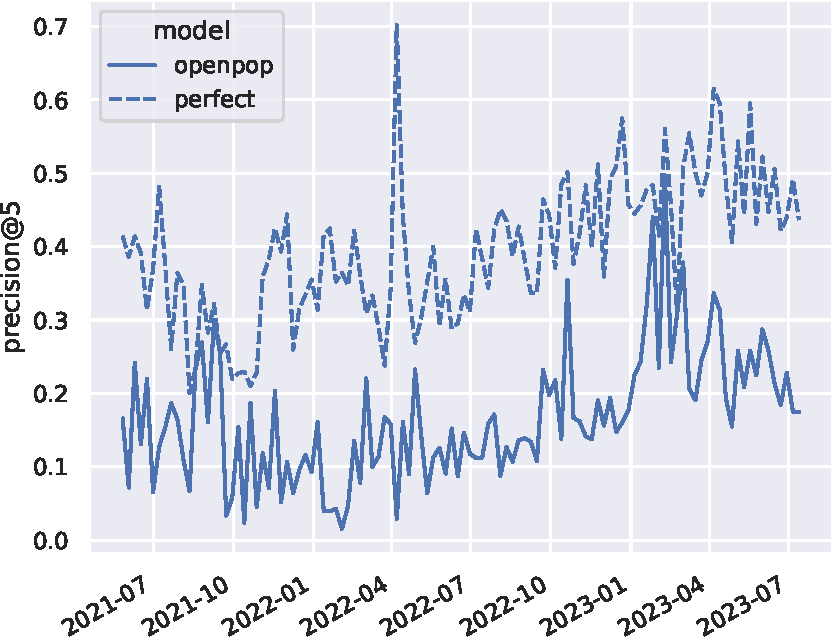
\includegraphics[width=\linewidth]{figures/04_validacion/10_all_precision@5_W-THU_True_Decentraland.pdf}
        \caption{Precisión en 5}
        \label{fig:openpop_precision@5}
    \end{subfigure}\hfill\begin{subfigure}{.48\textwidth}
        \centering
        % Source: 10_baseline_mp.ipynb [32]
        % Actualizado 2024-03-23
        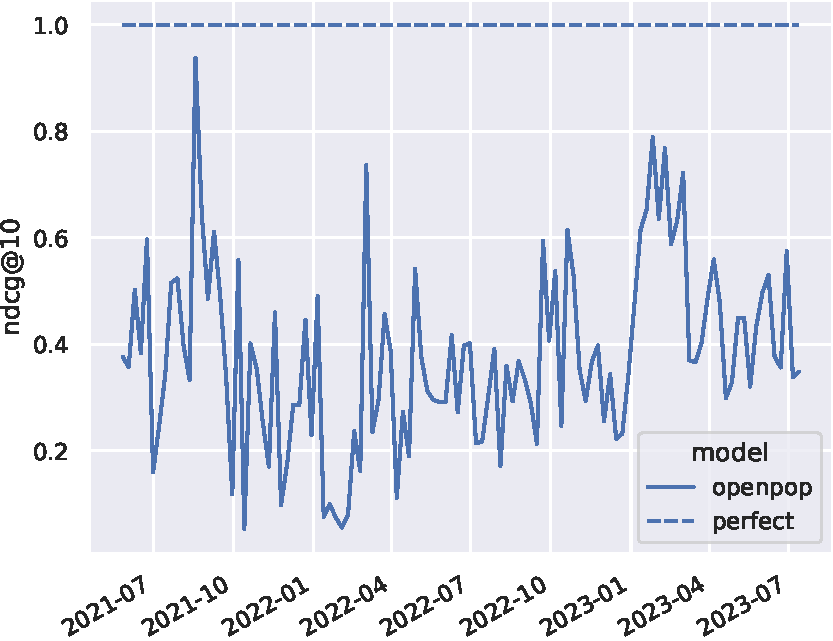
\includegraphics[width=\linewidth]{figures/04_validacion/10_all_ndcg@10_W-THU_True_Decentraland.pdf}
        \caption{nDCG en 10}
        \label{fig:openpop_ndcg@10}
    \end{subfigure}
    \caption[Resultados del modelo línea base.]{Resultados del modelo OpenPop (línea base) a lo largo de todos los folds disponibles.}
    \label{fig:openpop_results}
\end{figure}

Otra línea base utilizada, únicamente para compararlo con esta línea base, es el clasificador perfecto. Es necesario pues para algunas métricas utilizadas, al haber muy pocos votos disponibles en test por usuario, es imposible llegar a un valor de 1, como se explica en la sección~\ref{subsec:metricas}. Estos dos modelos y sus resultados se exploran en el \textit{notebook} \url{10_baseline_mp.ipynb} del repositorio del proyecto~\cite{davo_daviddavoupm-tfm-notebooks_2024}.


% Source: 10_baseline_mp.ipynb 
% Actualizado 2024-03-23
El análisis de los resultados del modelo OpenPop, utilizando la división de datos de la subsección~\ref{subsec:exploracion-folds}, revela una $\precision{5}$ media de $0.17\pm0.09$ en todos los folds. En comparación, un clasificador perfecto alcanza un valor de $0.39$, con un intervalo de confianza similar, lo que sugiere un amplio margen para mejorar el rendimiento del modelo. Esto indica que los usuarios no se limitan únicamente a las propuestas populares, e introducir personalización en las recomendaciones podría mejorarlas. Por otro lado, el valor medio del $\recall{5}$ es de $0.39\pm0.23$.

En términos de métricas de \textit{ranking}, el $\nDCG@10$ alcanza una media de $0.38\pm0.17$ a lo largo de todos los folds. Por definición, un clasificador perfecto obtendría un nDCG de 1. El $\MAP@10$ obtiene un valor de $0.28\pm0.16$.


La figura~\ref{fig:openpop_results} ilustra cómo la precisión, tanto en el caso perfecto como en la línea base, ha ido aumentando gradualmente con el tiempo, en paralelo al incremento de la participación. Sin embargo, el \gls{ndcg} es muy variable.

Es importante destacar que, para el entrenamiento y la validación de los modelos, se han utilizado exclusivamente los últimos 10 folds disponibles. En estos folds finales, la $\precision{5}$ de la línea base alcanza un valor de $0.22\pm0.04$ y la del modelo perfecto alcanza $0.47\pm0.06$, un valor significativamente más alto que en el resto de folds. Por su parte, el $\nDCG@10$ alcanza un valor de $0.42\pm0.09$, también mucho mejor.

% \begin{itemize}
%     % \item En todos los folds, el recomendador OpenPop consigue una $\precision{5}$ media de $0.17\pm0.09$, mientras que el clasificador perfecto consigue un valor de $0.39\pm0.09$, por lo que hay bastante hueco para mejora, dando a entender que los usuarios no se guían solo por las propuestas, y es necesario añadir personalización a las recomendaciones, aunque el modelo OpenPop no se queda atrás y es una línea base alta.
%     % \item El $\recall{5}$ medio es de $0.39\pm0.23$.
%     % \item En cuanto a métricas de ranking, el $\nDCG@10$ obtiene una media de $0.39\pm0.17$. El clasificador perfecto, por definición, tiene un \gls{ndcg} de 1. El $\MAP@10$ es de $0.28\pm 0.16$.
%     % \item Como se ve en la figura~\ref{fig:openpop_results}, la precisión, tanto perfecta como línea base, ha ido aumentando poco a poco, conforme a subido la participación a lo largo del tiempo. El \gls{ndcg}, sin embargo, es muy variable.
%     \item Sin embargo, como se especifica en la subsección~\ref{subsec:exploracion-folds}, para el entrenamiento y validación de los modelos solo se utilizan los últimos 10 folds disponibles. En estos últimos folds, la $\precision{5}$ base aumenta a $0.24\pm0.05$ con una $\precision{5}$ de $0.48\pm 0.06$ en el modelo perfecto. El $\nDCG@10$ es de $0.45\pm 0.09$.
% \end{itemize}


% \begin{itemize}
%     \item Dado un timestamp nuestro modelo baseline recomienda la propuesta abierta con más votos hasta el momento en la que el usuario aún no ha votado, y lo denominamos \acrfull{openpop}. Puede considerarse una modificación del modelo \textit{RecentPop} de \textcite{ji_re-visit_2020}, pero teniendo en cuenta el cierre de las propuestas.
%     \item A efectos de implementación, dado un conjunto de entrenamiento y test separados como se especifica en la sección~\ref{sec:division_datos}, simplemente es necesario contar el número de votos en entrenamiento de las propuestas abiertas, es decir, que están en ambos conjuntos.
% \end{itemize}

% \section{Entrenamiento de los modelos}
% \label{sec:entrenamiento_modelos}

% \begin{itemize}
%     \item En todos los casos se crea un nuevo modelo para cada fold, no se exprime nada del conocimiento aprendido.
%     \item Por esa razón
% \end{itemize}

% De esta manera, el modelo se ejecutará en intervalos discretos de tiempo, y la evaluación será en consecuencia. Es decir, asumiendo que el recomendador se ejecutará de forma periódica (por ejemplo, cada semana o cada día) y se evaluará de acuerdo con esta periodicidad. No se contempla la ejecución continua, sino que presupone la posibilidad de reentrenar completamente el modelo en cada ocasión que se desee realizar nuevas recomendaciones. Por consiguiente, uno de los requisitos es que el entrenamiento de los sistemas desarrollados sea rápido, con tiempos de entrenamiento en el orden de minutos.

\chapter{Implementación y experimentos}
\label{ch:implementacion_experimentos}

\section{Obtención de datos}
\label{sec:obtencion-datos}

Para la obtención de datos se ha utilizado el \textit{DAO Analyzer dataset}~\cite{arroyo_dao_2024}, el único dataset sobre \glspl{dao} disponible en Kaggle o Zenodo a fecha de comienzo de este proyecto. Este dataset incluye datos de organizaciones en Aragon, DAOstack y DAOhaus, y en el que ha participado anteriormente el autor de este proyecto. Durante el desarrollo del TFM se ha modificado ligeramente el dataset para obtener la información textual (título y descripción) de las propuestas realizadas. Además, se ha aumentado este dataset con las \glspl{dao} de la plataforma Snapshot, utilizando parte de los scripts desarrollados durante la pasantía de verano de Andrew Schwartz en el Departamento de Ingeniería del Software e Inteligencia Artificial de la Universidad Complutense de Madrid, aunque también han necesitado ser modificados para descargar la información textual de las propuestas. Finalmente, los datos han sido publicados en Kaggle~\cite{tfm-dataset-text}.

Debido a que sólo se han explorado organizaciones de las plataformas Aragon, DAOstack, DAOhaus y Snapshot, en esta sección solo se explorará la obtención de datos de estas plataformas, aunque las herramientas utilizadas son capaces de más.

En la figura~\ref{fig:daos-census} puede verse un resumen de las fuentes de los datos y los procesos realizados para la elaboración del dataset.

\begin{figure}[tbh]
    \centering
    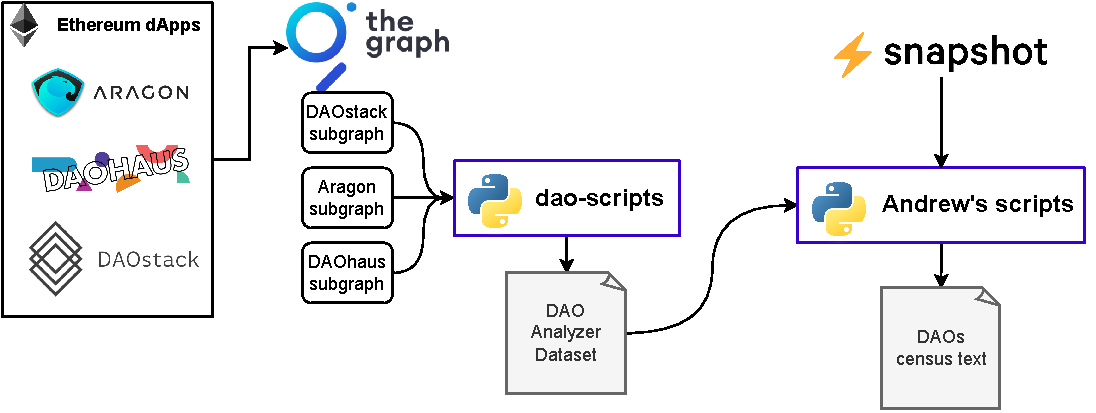
\includegraphics[width=\linewidth]{figures/04_implementacion/daos-census-Horizontal.drawio.pdf}
    \caption{Esquema de la obtención de datos de las plataformas para su posterior análisis.}
    \label{fig:daos-census}
\end{figure}

\subsection{Aragon, DAOhaus y DAOstack}

Para obtener los datos de las organizaciones de las plataformas Aragon, DAOstack y DAOhaus, el paquete dao-scripts~\cite{arroyo_dao-analyzer_2022} utiliza el servicio The Graph\footnote{\url{https://thegraph.com/}}, una plataforma que permite indexar y consultar datos de \glspl{dapp} de manera eficiente. Por como funciona la blockchain, la manera de conocer el estado actual de un programa en ejecución es descargarse toda la cadena de bloques y recorrerla bloque a bloque realizando las operaciones de reducción necesarias, de igual modo que para conocer el saldo de una cuenta bancaria es necesario computar todas las transferencias realizadas. The Graph provee de indexadores gratuitos que realizan esta tarea y dispone los resultados mediante una API en GraphQL, lo que evita tener un servidor indexando solo para nuestra aplicación. 

Para desplegar un subgrafo (cada uno de los repositorios de información indexada asociados a una \gls{dapp}) es necesario programar en Typescript el código que ejecutará el indexador, y para ello es necesario tener acceso al código fuente de los contratos inteligentes que forman la aplicación. Esta tarea ya la realizaron los creadores de las tres plataformas y por lo tanto los subgrafos ya están desplegados.

Sin embargo, muchas de estas plataformas han abandonado su desarrollo, por lo que ha sido necesario realizar cierto mantenimiento y en ocasiones añadir información necesaria para que pueda ser obtenida por los scripts en los subgrafos de Aragon y DAOstack.

El programa que obtiene los datos de The Graph, los empaqueta en formato Arrow o \gls{csv} y los sube a Zenodo y Kaggle se llama dao-scripts y el código en Python está disponible en GitHub\footnote{\url{https://github.com/Grasia/dao-scripts}}. Los datos son obtenidos diariamente con un GitHub action y actualizados tanto en Zenodo como en Kaggle, en un conjunto conocido como \textit{DAO Analyzer Dataset} y al que habría que añadir las organizaciones de Snapshot, como se explicará en la próxima sección. Los ficheros \gls{csv} que forman el conjunto de datos ocupan 130MB, de los cuales aproximadamente 100MB son la información textual de las propuestas.

\subsection{Snapshot}

En el caso de Snapshot, al ser una plataforma \textit{off-chain}, es decir, no desplegada en la blockchain, no podemos utilizar The Graph. Sin embargo, Snapshot utiliza su propia API GraphQL\footnote{\url{https://hub.snapshot.org/graphql}}, por lo que puede reutilizarse parte del código y de los algoritmos desarrollados en los dao-scripts. Sin embargo, debido al diferente esquema de la API~\cite{snapshot_snapshot_nodate}, además de problemas de escalabilidad inherentes a su popularidad y la gran actividad con la que cuenta, Andrew Schwartz hizo estos scripts casi de cero en Jupyter Notebooks. Posteriormente, realicé un \textit{fork} en GitHub\footnote{\url{https://github.com/daviddavo/daos-verano}} de dichos scripts, añadiendo algunas utilidades y, sobre todo, obteniendo la información textual de las organizaciones desplegadas en Snapshot.

Finalmente, estos notebooks combinan los datos del \textit{DAO Analyzer dataset} con los obtenidos de Snapshot para crear un nuevo conjunto de datos aumentado, denominado \citetitle{tfm-dataset-text} y disponible en Kaggle~\cite{tfm-dataset-text}. Este nuevo dataset está formado por ficheros en formato Parquet debido a su escala, y ocupa 3.63 GB. En este caso, el gran espacio ocupado es debido a la información sobre los votos, que ocupa aproximadamente 3.55 GB. La información textual de las propuestas ocupa tan solo 45 MB, y el resto de datos de las propuestas y organizaciones ocupa 32 MB.

La sección~\ref{sec:explora_datos} abordó la exploración de este conjunto de datos.

\section{Preparación de datos}

Para garantizar la reutilización del código de preparación de datos en todos los notebooks, se ha creado el módulo \url{src.datasets}, cuyo código está disponible en el GitHub del proyecto~\cite{davo_daviddavoupm-tfm-notebooks_2024}.

La extracción de los conjuntos de datos se realiza mediante la API de Kaggle, empleando el formato Apache Parquet para su almacenamiento. Dado el tamaño considerable de estos conjuntos, se ha optado por la utilización de DuckDB~\cite{raasveldt_duckdb_2023} para realizar consultas de filtrado, permitiendo así una manipulación eficiente de los datos. Posteriormente, se transforman los resultados en estructuras de datos manejables mediante Pandas DataFrame~\cite{mckinney_data_2010}.

Este proceso de preparación de datos se encapsula en el método \url{get} del módulo \url{src.datasets.daocensus}. Dicho método, al ser invocado con el nombre específico de la \gls{dao}, devuelve dos DataFrames distintos: uno que contiene todas las propuestas y otro que contiene los votos relacionados con dichas propuestas. Además, esta función es capaz de realizar la descarga automática de los conjuntos de datos desde Kaggle si estos aún no se encuentran disponibles, y permite la aplicación de filtros según la plataforma y el número mínimo de votos por propuesta.

Además, se ha implementado un proceso de estandarización de los datos para adecuarlos al formato comúnmente utilizado por los modelos de la librería \url{microsoft/recommenders}~\cite{argyriou_microsoft_2020}. Para ello, se ha desarrollado el método \url{to_microsoft}, el cual convierte el DataFrame de votos en un DataFrame de interacciones con tres columnas: \textit{userID}, \textit{itemID} y \textit{rating} (siendo este último siempre igual a 1 debido a que se trata de un \textit{feedback} implícito).

También se ha facilitado la carga del conjunto de datos en forma de grafo utilizando un formato basado en pares de tensores, para su uso en PyTorch Geometric~\cite{fey_fast_2019}. A pesar de no haberse utilizado dicha librería en la implementación final, esta opción se mantiene disponible para futuras investigaciones o análisis que puedan requerir este tipo de representación de los datos.

\section{Especificaciones de los sistemas recomendadores}

Se han desarrollado dos sistemas recomendadores siguiendo dos enfoques distintos: uno basado en contenido y otro basado en la relación entre los usuarios y las propuestas, también conocido como \acrfull{cf}.

Además, se ha explorado la posibilidad de crear un sistema recomendador híbrido que combine las recomendaciones generadas por estos dos modelos.

A continuación, se detallan en profundidad estos tres sistemas desarrollados para ofrecer una comprensión exhaustiva de sus características, funcionamiento y resultados.

Para el desarrollo de los sistemas se han utilizado únicamente los datos de la organización Decentraland, aunque en el capítulo~\ref{ch:resultados_discusion} se presentan los resultados de utilizar el sistema en otras organizaciones.

\subsection{Sistema basado en contenido}
\label{subsec:implementacion-contenido}

El enfoque del sistema basado en contenido se fundamenta en el análisis de la información textual asociada a las propuestas. En este contexto, la disponibilidad de datos se reduce al título y la descripción de cada propuesta. Es importante tener en cuenta que no todas las propuestas contienen este tipo de información. Para abordar este problema, se ha decidido un enfoque pre-entrenado que permita aprovechar modelos de \gls{pln} previamente entrenados en grandes conjuntos de datos textuales.

La selección de un modelo pre-entrenado se justifica por la moderada cantidad de datos disponibles y la naturaleza semi-supervisada del aprendizaje. Este enfoque ofrece la ventaja de utilizar representaciones de texto de alta calidad aprendidas en corpus de datos extensos, lo que puede mejorar significativamente el rendimiento del modelo.

Un aspecto clave en el procesamiento de la información textual de las propuestas es la naturaleza específica del lenguaje utilizado. En muchas ocasiones, las propuestas abordan temas técnicos con terminología especializada o incluyen jerga propia de la \gls{dao}. Esto plantea desafíos adicionales para el modelado del contenido, ya que un enfoque tradicional de bolsa de palabras (\textit{bag-of-words}) podría resultar inadecuado. En su lugar, se requiere un enfoque que capture la semántica subyacente de las palabras y sea capaz de manejar términos derivados y neologismos específicos del dominio. Por ejemplo, aunque la palabra \textquote{Decentraland} no se encuentre en el corpus, debería tener una representación similar a la de \textquote{Descentralización}.

Comparado con el enfoque de filtrado colaborativo, el sistema basado en contenido presenta la ventaja de evitar el problema del arranque en frío (\textit{cold start}) para las propuestas. Desde el momento de su creación, el sistema puede generar recomendaciones basadas en el contenido textual disponible. Sin embargo, se ha seguido un enfoque de evaluación similar al de los otros sistemas para garantizar la comparabilidad de los resultados y la robustez de la evaluación.

En la generación del espacio latente de las propuestas, se concatena el título y la descripción de cada propuesta para generar un \textit{embedding} de texto representativo. Es importante destacar que este \textit{embedding} permanece constante durante toda la vida útil de la propuesta, lo que permite generar recomendaciones desde el momento de su creación y mantener la consistencia en las recomendaciones a lo largo del tiempo.

El impacto del tiempo se refleja en la evolución del modelo de los usuarios, que puede ser influenciado por su interacción con nuevas propuestas. Sin embargo, los \textit{embeddings} de las propuestas permanecen inalterados. En las secciones siguientes de este capítulo, se exploran dos modelos que hemos considerado para aplicar a cada usuario y realizar recomendaciones: el basado en similitud del coseno y el enfoque \gls{knn}.

Para la generación de los \textit{embeddings} de las propuestas, se ha utilizado el modelo \url{all-mpnet-base-v2} de la librería de Python Sentence Transformers~\cite{reimers_sentence-bert_2019}, que utiliza redes de tipo \gls{bert}.

El código utilizado para desarrollar y evaluar estos modelos se encuentra disponible en el notebook \url{11_pln_tune} del repositorio GitHub del proyecto~\cite{davo_daviddavoupm-tfm-notebooks_2024}. A partir de las pruebas realizadas en el notebook, se ha creado una clase del modelo de similitud de coseno, la cual está disponible en la clase \url{src.models.NLPSimilarity} del repositorio.

\subsubsection{Similitud del usuario}

% \begin{itemize}
%     \item Cada usuario tiene un embedding que es igual a la suma normalizada de los embeddings de las propuestas en las que ha votado (sin importar si fue a favor o en contra).
%     \item Se recomiendan las $k$ propuestas con mejor similitud del coseno con el embedding del usuario.
%     \item Lo bueno (y lo malo) es que no es parametrizable. Hay un hiperparámetro menos entre los que buscar, pero tal vez se pueda ajustar mejor a este caso.
%     \item Aunque no se ha implementado así, una gran ventaja es que la operación de la suma sobre una ventana temporal puede realizarse con coste constante $\mathcal{O}(1)$ \cite{hirzel_sliding-window_2017}
%     \item La media del MAP de este recomendador entre todos los folds es de $0.31\pm 0.08$
%     \item Además, se probó a reducir el número de propuestas usadas para recomendar, en lugar de usar todo el conjunto de entrenamiento (fue por casualidad, pero no sé si decir eso xD). 
%     \item Resulta que usar solamente las propuestas en las que ha votado el usuario durante los últimos 14 días mejora notablemente las recomendaciones con respecto a usar todo el dataset, y además se tarda menos en calcular los embeddings del usuario pues hay menos propuestas que agregar.
%     \item Se ha realizado una grid search con distintos tamaños de ventana de 7 días a 1 año. Se muestran los resultados en la figura~\ref{fig:pln-similairity_results}.
%     \item Lo mejor parece ser utilizar solo 14d de propuestas. En concreto, la $map@5$ sube de $0.31\pm 0.08$ a $0.40\pm 0.11$ si utilizamos una ventana de 14 días en lugar de usar todas las propuestas. El tiempo de ejecución se reduce en 4, de 80ms a 20ms.
% \end{itemize}

Cada usuario está representado por un \textit{embedding}, el cual se obtiene como la suma normalizada de los \textit{embeddings} de las propuestas en las que ha emitido un voto, ya sea a favor o en contra. La recomendación está formada por las $k$ propuestas con mayor similitud del coseno con el \textit{embedding} del usuario.

Este enfoque se distingue por su rapidez tanto en el entrenamiento como en la ejecución. Dado que no requiere ajustar hiperparámetros, el proceso de entrenamiento es ágil y no implica iteraciones para encontrar configuraciones óptimas. Aunque en la implementación actual no se utiliza una ventana temporal, la operación de suma sobre una ventana temporal tiene un costo constante $\mathcal{O}(1)$ \cite{hirzel_sliding-window_2017}, lo que garantizaría eficiencia y escalabilidad, independientemente del tamaño del conjunto de datos.

\begin{figure}[t]
    \begin{subfigure}{.48\textwidth}
        \centering
        % Source: 11_pln-tune.ipynb [29]
        % Actualizado 2024-04-10 
        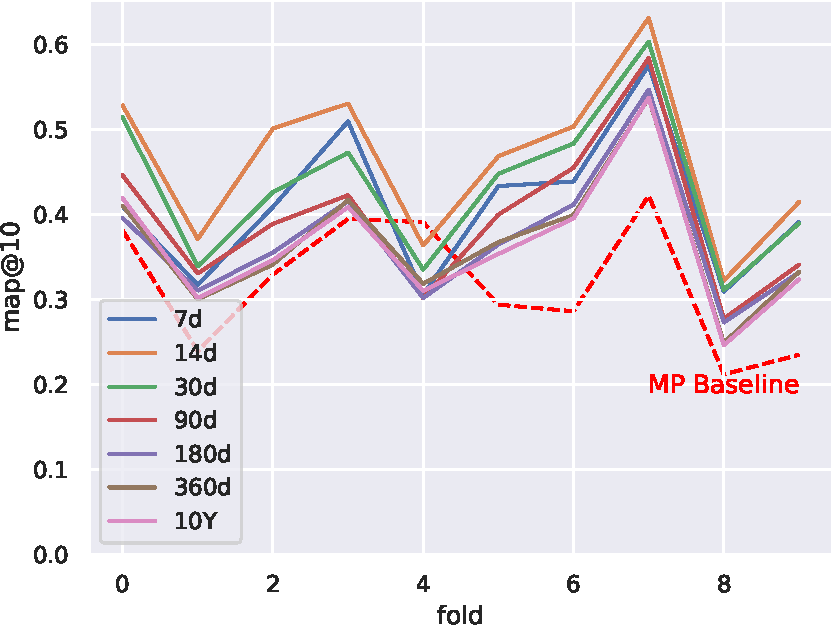
\includegraphics[width=\linewidth]{figures/04_implementacion/11_cosine_results_results-lines_W-THU_normalize=True.pdf}
        \caption{Precisión obtenida en cada fold.}
    \end{subfigure}\hfill\begin{subfigure}{.48\textwidth}
        \centering
        % Source: 11_pln-tune.ipynb [30]
        % Actualizado 2024-04-10
        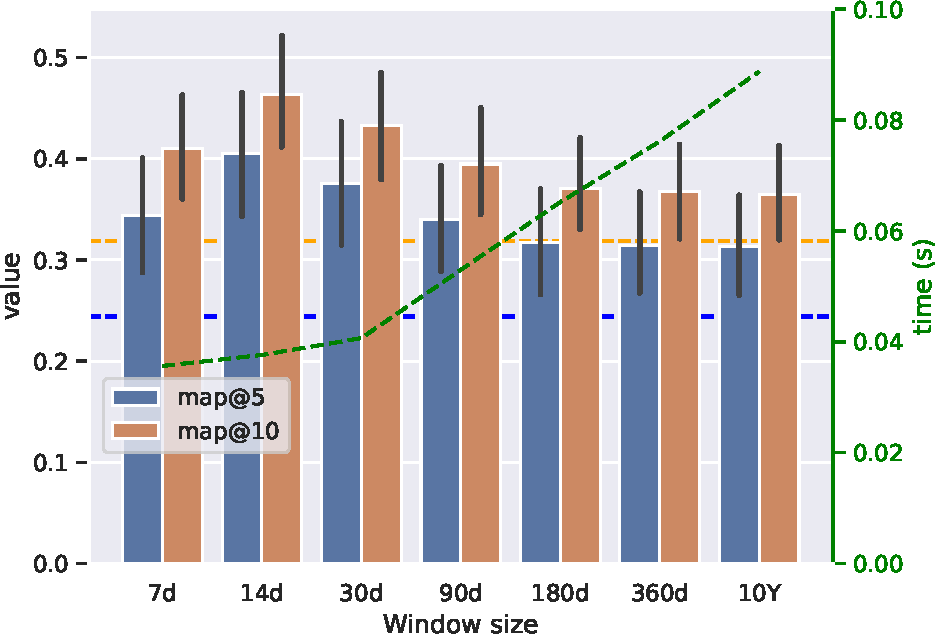
\includegraphics[width=\linewidth]{figures/04_implementacion/11_cosine_results_window-size_W-THU_normalize=True.pdf}
        \caption{Media entre todos los folds. Las barras de error representan el \acrshort{ic}.}
        \label{fig:pln-similarity_window-size}
    \end{subfigure}
    \caption[Resultados del sistema recomendador basado en similitud del coseno en Decentraland.]{Resultados del sistema recomendador basado en similitud con el usuario entre propuestas y usuarios dependiendo del tamaño de la ventana de propuestas en Decentraland. En rojo la línea base del clasificador más votado.}
    \label{fig:pln-similairity_results}
\end{figure}

% Source: 11_pln-tune.ipynb [26] Column 10 years
% Actualizado 2024-04-10
El rendimiento medio del MAP@10 de este recomendador en todos los folds es de $0.36\pm 0.08$. Se realizó un experimento para evaluar el impacto de reducir el número de propuestas utilizadas para realizar las recomendaciones y se observó que limitar las propuestas a aquellas en las que el usuario ha votado durante los últimos 30 días mejoraba significativamente la calidad de las recomendaciones en comparación con el uso de todo el conjunto de datos. Además, este enfoque reduce el tiempo de cálculo de los \textit{embeddings} del usuario debido a la menor cantidad de propuestas a considerar.

Se llevó a cabo una búsqueda en rejilla (\textit{grid search}) con diferentes tamaños de ventana, variando desde 7 días hasta 1 año. Los resultados se presentan en la figura~\ref{fig:pln-similairity_results}. Se observó que el uso de una ventana de 14 días resulta óptimo, ya que el $map@10$ aumenta de $0.36\pm 0.08$ a $0.46\pm 0.09$, en comparación con el uso de todo el conjunto de propuestas. Además, el tiempo de ejecución se reduce de 86ms a 36ms. Hay que tener en cuenta que el tiempo de ejecución no incluye el cálculo de los \textit{embeddings}, que está cacheado, aunque el servidor (véase~\ref{ch:servidor}) tarda a penas 5 segundos en calcular los \textit{embeddings} de las 1950 propuestas, utilizando el modelo \url{all-mpnet-base-v2}.

\subsubsection{K vecinos más cercanos}

% \begin{itemize}
%     \item Cada usuario tiene su propio modelo \gls{knn} en el que los datos son las propuestas en las que ha votado o no, y se intenta clasificar una propuesta nueva haciendo la agregación de los k vecinos más cercanos. Se ha utilizado la clase \url{KNeighborsClassifier} de scikit learn~\cite{pedregosa_scikit-learn_2011}.
%     \item Debido a que muchos usuarios han votado poco, se hace \textit{fallback} al modelo most popular en el caso de que el $k$ del \gls{knn} sea mayor que el número de propuestas en las que ha votado el usuario. Esto hace que cuanto mayor sea la $k$, se haga menos uso de \gls{knn} y más del fallback. 
%     \item Sin embargo, aumentar el tamaño de la ventana añade más propuestas al entrenamiento, por lo que aumenta el porcentaje de uso de knn. Ambos casos se ven ilustrados en la figura~\ref{fig:knn_usage}. Obviamente, cambiar la métrica utilizada no afectará al porcentaje de uso de \gls{knn}.
%     \item Además, debido a la baja cantidad de muestras negativas, habrá una sobre-representación de muestras. Por ello hacemos un sampling en el que el número de muestras negativas es igual al número de muestras positivas.
%     \item Hay que tener en cuenta que como el feedback es implícito, una muestra negativa no implica que al usuario no le hubiese interesado la propuesta, seguramente no haya votado en ella porque no estaba disponible en ese momento.
%     \item Es necesario hacer una búsqueda de hiperparámetros en k, además mantenemos lo del tamaño de la ventana. También se ha probado a usar tanto la distancia del coseno como la minkowski, realizando una búsqueda en una rejilla de 196 puntos, definida por el espacio de la tabla~\ref{tab:knn_espacio_busqueda}.
%     \item Sin embargo, da igual, pues a penas supera la línea base del más votado. Esto es debido a que tenemos muy poco feedback positivo, por lo que las muestras negativas en realidad son muy parecidas a otros vecinos positivos.
%     \item El resumen de los resultados de la búsqueda está en la figura~\ref{fig:knn_results_all}. En general, coger cualquiera de las dos maneras para medir la distancia no influye en los resultados, y el mejor valor de $k$ parece ser 1 independientemente del tamaño de la ventana. Cuando la $k$ es demasiado alta, acaba haciendo uso tan solo del fallback, que no realiza recomendaciones personalizadas. En cuanto al tamaño de la ventana, parece ser que lo mejor es coger las propuestas en las que el usuario ha votado en los últimos 360 días, contrastando con el de similitud con el usuario, en el que la mejor opción era coger tan sólo los últimos 14 días. La mejor opción (k=1, window=360d, metric=cosine) tiene como resultado un MAP@10 de $0.44\pm0.11$. Supera en 4 puntos al modelo de similitud con el usuario sin optimizar, pero la versión optimizada supera a este por 8 puntos.
%     \item Sobre el tiempo de ejecución (véase figura~\ref{fig:knn_results_time}), este modelo es 300 veces más lento que el modelo basado en similitud con el usuario, pasando del orden de los 50ms a 15 segundos. El otro modelo realiza una simple suma y calcula la distancia del usuario a todas las propuestas, mientras que este modelo necesita calcular la distancia de todas las propuestas entre sí. Y eso que he hecho sampling para quitar ejemplos negativos.
% \end{itemize}

En el enfoque de \acrfull{knn}, cada usuario posee su propio modelo donde los datos son las propuestas en las que ha votado o no. Se intenta clasificar una nueva propuesta en dos clases (votará/no votará) mediante la agregación de los $k$ vecinos más cercanos. El \textit{score} de una predicción será el porcentaje de vecinos de la nueva propuesta en los que el usuario ha votado. Para esto, se ha empleado la clase \url{KNeighborsClassifier} de scikit-learn~\cite{pedregosa_scikit-learn_2011}.

Dado el bajo número de muestras positivas, se realiza un muestreo donde el número de muestras negativas es igual al número de muestras positivas. Es importante destacar que, dado que el feedback es implícito, una muestra negativa no indica necesariamente que al usuario no le habría interesado la propuesta. Es probable que el usuario no haya votado en ella porque no estaba disponible en ese momento.

Debido a que muchos usuarios han emitido pocos votos, se realiza un \textit{fallback} al modelo línea base Más Popular (véase~\ref{sec:linea_base}) en el caso de que el valor de $k$ en el \gls{knn} sea mayor que el número de propuestas en las que ha votado el usuario. Esto implica que a medida que $k$ aumenta, se reduce el uso del \gls{knn} y se incrementa el del \textit{fallback}, como puede observarse en la figura~\ref{fig:knn_usage_k}.

\begin{figure}[t]
    \centering
    \begin{subfigure}{.48\textwidth}
        \centering
        % Source: 11_pln-tune.ipynb [42]
        % Actualizado 2024-04-10
        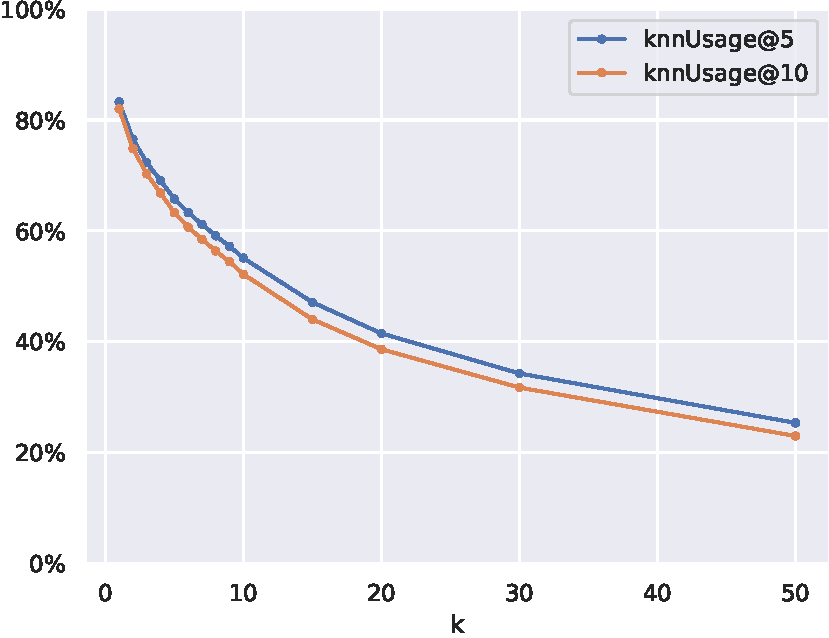
\includegraphics[width=\linewidth]{figures/04_implementacion/11_knn_usage_k_W-THU_normalize=True.pdf}
        \caption{Porcentaje medio de uso de knn para los distintos $k$ probados.}
        \label{fig:knn_usage_k}
    \end{subfigure}\hfill\begin{subfigure}{.48\textwidth}
        \centering
        % Source: 11_pln-tune.ipynb [43]
        % Actualizado 2024-04-10
        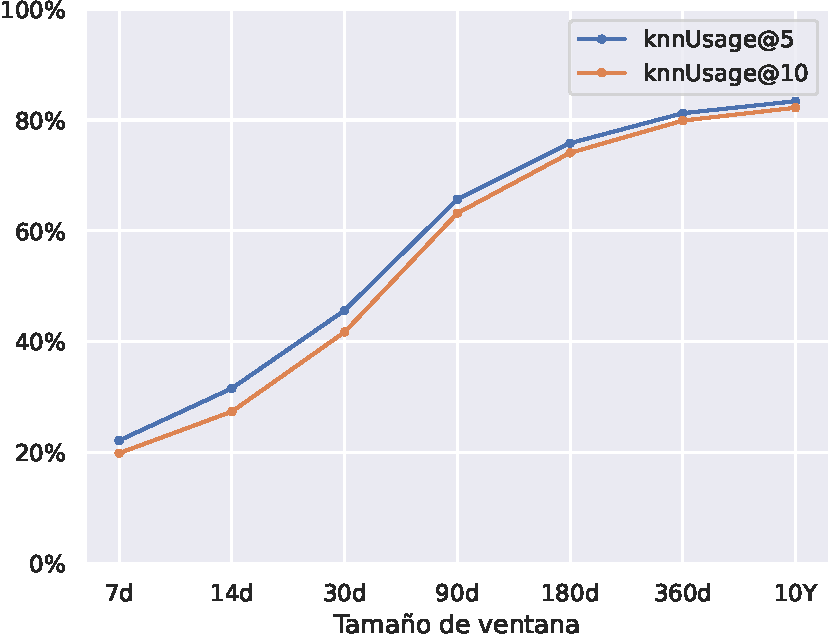
\includegraphics[width=\linewidth]{figures/04_implementacion/11_knn_usage_window_size_W-THU_normalize=True.pdf}
        \caption{Porcentaje medio de uso de knn en cada tamaño de ventana.}
        \label{fig:knn_usage_window_size}
    \end{subfigure}
    \caption[Porcentaje de uso de \acrshort{knn} vs el \textit{fallback} variando hiperparámetros.]{Porcentaje de uso de \gls{knn} vs el \textit{fallback} variando dos hiperparámetros.}
    \label{fig:knn_usage}
\end{figure}

Al igual que en el modelo anterior, se ha decidido probar distintas ventanas temporales de entrenamiento para comprobar el rendimiento del modelo. El tamaño de esta ventana impacta en la cantidad de propuestas incluidas en el entrenamiento, afectando así el porcentaje de uso del \gls{knn}. Este efecto se observa en la figura~\ref{fig:knn_usage_window_size}. También se ha probado el modelo con distintas métricas de distancia entre las muestras. Sin embargo, cambiar la métrica de distancia no afectará al porcentaje de uso del \gls{knn}.

Para utilizar \gls{knn}, es necesario llevar a cabo una búsqueda del hiperparámetro $k$. Además, usamos distintos tamaños de ventana de propuestas a considerar como en el modelo anterior, y probamos tanto con la distancia del coseno como la Euclídea (Minkowski con $p=2$). Se ha realizado la búsqueda con una rejilla de 196 puntos, definida por el espacio en la tabla~\ref{tab:knn_espacio_busqueda}.

\begin{table}
    \centering
    \begin{tabular}{l|c}
        \toprule
        \textbf{Hiperparámetro} & \textbf{Valores} \\
        \midrule
        Window size & $ \{ 7d,14d,30d,90d,180d,360d,10Y \} $ \\
        k vecinos & $ [1,10] \cup \{15,20,30,50\}$ \\
        Métrica & \{ Euclídea, Similitud del coseno \} \\
        \bottomrule
    \end{tabular}
    \caption{Espacio de búsqueda de hiperparámetros para la optimización del modelo basado en \gls{pln} y \gls{knn}.}
    \label{tab:knn_espacio_busqueda}
\end{table}

El resumen de los resultados de la búsqueda se muestra en la figura~\ref{fig:knn_results_all}. En general, la elección de la medida de distancia apenas influye en los resultados, y el mejor valor de $k$ parece ser 1 (\textit{Nearest neighbor}) independientemente del tamaño de la ventana. Además, cuando $k$ es demasiado alto, el modelo acaba recurriendo únicamente al \textit{fallback}, lo que no ofrece recomendaciones personalizadas.

En cuanto al tiempo de ejecución (véase figura~\ref{fig:knn_results_time}), este modelo es 300 veces más lento que el basado en similitud con el usuario, con tiempos de ejecución de alrededor de 15 segundos para los hiperparámetros que maximizan el \gls{map}. A diferencia del otro modelo, que realiza una simple suma y calcula la distancia del usuario a todas las propuestas, este necesita calcular la distancia entre todas las propuestas entre sí. Se ha realizado un muestreo para eliminar ejemplos negativos, lo que sugiere que el tiempo de ejecución podría ser aún mayor sin este proceso.

\begin{figure}
    \begin{minipage}{.48\textwidth}
        % Source: 11_pln-tune.ipynb [45]
        % Actualizado 2024-04-10
        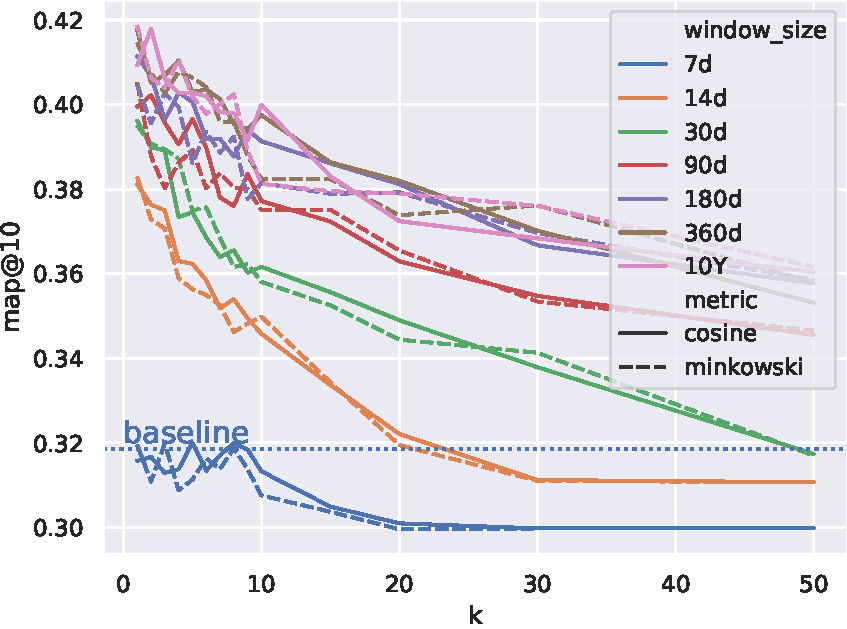
\includegraphics[width=\linewidth]{figures/04_implementacion/11_knn_results_all_W-THU_normalize=True.pdf}
        \caption{Resultados de la búsqueda de hiperparámetros para el modelo \acrshort{knn}}
        \label{fig:knn_results_all}
    \end{minipage}%
    \hfill%
    \begin{minipage}{.48\textwidth}
        % Source: 11_pln-tune.ipynb [46]
        % Actualizado 2024-04-10
        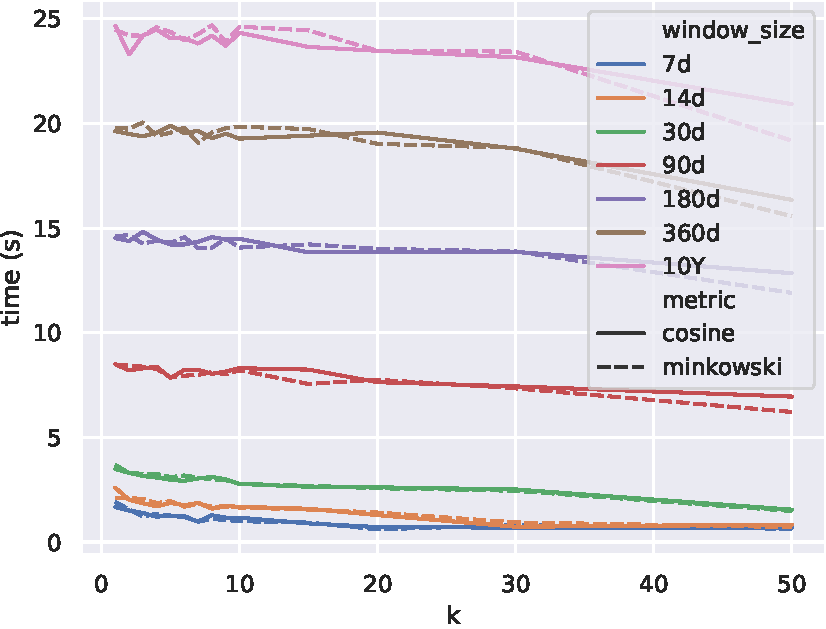
\includegraphics[width=\linewidth]{figures/04_implementacion/11_knn_results_time_W-THU_normalize=True.pdf}
        \caption{Tiempo de ejecución con varios hiperparámetros con el modelo \acrshort{knn}}
        \label{fig:knn_results_time}
    \end{minipage}
\end{figure}

\subsection{Sistema basado en filtrado colaborativo}
\label{subsec:implementacion-colaborativo}

Esta estrategia se basa en aprovechar el grafo de relaciones entre los usuarios como parte del \gls{sr}. Esta aproximación permite capturar conexiones sociales y patrones emergentes en la interacción entre usuarios, incluso cuando la información sobre las propuestas en sí es limitada. Sin embargo, estas propuestas se desenvuelven en comunidades, donde surgen dinámicas específicas y existen estructuras sociales latentes, al igual que en el caso del Software Libre~\cite{bird_latent_2008}.

En términos más específicos, se ha desarrollado un sistema de filtrado colaborativo basado en aprendizaje profundo, utilizando en particular una \acrfull{gnn}. La intención es poder expandir el grafo en el futuro incorporando otras interacciones de los usuarios, incluso aquellas que ocurren fuera de la organización o de otras \glspl{dapp}, como las transferencias de dinero. Para esta implementación, se ha optado por utilizar el modelo LightGCN~\cite{he_lightgcn_2020}, disponible en la librería microsoft/recommenders~\cite{argyriou_microsoft_2020}. Este modelo se ha seleccionado debido a su actualidad, rendimiento sólido, y su eficiencia computacional (similar a una factorización de matrices), además de haber sido probado en diversos conjuntos de datos y \textit{benchmarks}. 

Es importante subrayar que el propósito principal de este proyecto no radica en la creación ni en el desarrollo de nuevos modelos, sino en la aplicación de los \acrlongpl{sr} a las \glspl{dao}. El funcionamiento del modelo se explica en profundidad en la subsubsección~\ref{subsubsec:lightgcn}.

En cuanto al entrenamiento y ajuste de hiperparámetros del modelo, se ha utilizado la librería Ray Tune~\cite{liaw_tune_2018}. Ha sido necesario modificar ligeramente las siguientes partes de la implementación del modelo:

\begin{itemize}
    \item Se incorporó un post-filtrado que evita recomendar propuestas que no están abiertas. Para ello, se ajustó la función \texttt{recommend\_k\_items}, la cual ahora recibe una lista de propuestas \textit{recomendables} (es decir, actualmente abiertas). Aquellas recomendaciones que no estén en esta lista se les asigna un \textit{score} de $-\infty$, de ese modo al hacer el \textit{ranking} de propuestas aparecerán las últimas y no serán recomendadas.
    \item Se introdujo el método \texttt{fit\_epoch} para realizar el fit de una sola época, permitiendo la detención temprana y permitiendo reportar las métricas con mayor granularidad en Ray Tune.
\end{itemize}

Este modelo modificado está disponible en la clase \texttt{LightGCNCustom}, ubicada en el módulo \texttt{src.models.lightgcn} del repositorio del TFM en GitHub~\cite{davo_daviddavoupm-tfm-notebooks_2024}. 

El espacio de búsqueda de hiperparámetros es continuo, por lo que se realiza una búsqueda metaheurística en este espacio usando HyperOpt~\cite{bergstra_making_2013}, pues es el único algoritmo de búsqueda de Ray Tune que permite la búsqueda en un espacio que mezcle hiperparámetros con valores continuos y discretos. En la tabla~\ref{tab:lightgcn_espacio_busqueda} se muestran los valores que definen el espacio de búsqueda utilizado.

\begin{table}[tbh]
    \centering
    \begin{tabular}{l|cc}
        \toprule
        \textbf{Hiperparámetro} & \textbf{Valores} & \textbf{Muestreo} \\
        \midrule
        Batch size & $bs\in\{ 64, 128, 256, 512, 1024 \} $ & Uniforme \\
        Embedding dim & $e\in\mathbb{N}, 1 \leq e \leq 1024$ & Loguniforme \\
        Capas de convolución & $c\in \{1,2,3,4,5,6\} $ & Uniforme \\
        Learning rate & $lr\in\mathbb{R}, 10^{-4} \leq lr \leq 1$ & Loguniforme \\
        Regularización L2 & $l2\in\mathbb{R}, 10^{-7}\leq l2 \leq 10^{-2}$ & Loguniforme \\ 
        \bottomrule
    \end{tabular}
    \caption{Espacio de búsqueda de hiperparámetros para la optimización del modelo LightGCN.}
    \label{tab:lightgcn_espacio_busqueda}
\end{table}

Asumimos que el modelo se reentrena cada vez que se requiere actualizar las recomendaciones. En consecuencia, no tiene sentido utilizar el mismo conjunto de hiperparámetros para el modelo en diferentes folds; se considera posible ajustar los hiperparámetros para generar nuevas recomendaciones. Por lo tanto, se optimiza la búsqueda de hiperparámetros en cada uno de los folds.

Sobre la generación de estos folds, se proporciona una explicación detallada en la sección~\ref{sec:division_datos}. Para cada uno de los 10 folds, se realizan 100 muestras. Las primeras 20 muestras son el punto de partida de HyperOpt. Aunque normalmente se utilizan muestras aleatorias, uno de los puntos de inicio es la mejor muestra del fold anterior.

La búsqueda intenta maximizar la métrica objetivo MAP@10. Se observó que utilizar la función de pérdida \gls{bpr} generaba sobre-aprendizaje, ya que resultaba en un valor de pérdida muy bajo, pero la precisión no alcanzaba niveles aceptables por encima de la línea base. Además, intentar optimizar la precisión o exhaustividad tampoco daba buenos resultados al ignorar por completo el orden de las recomendaciones. Sin embargo, un mejor \gls{map} sí se corresponde con una mejor precisión, como puede verse en la figura~\ref{fig:scatter_map_precision}. También podría haberse usado el \gls{ndcg}, pues son métricas similares y que están correlacionadas, como puede observarse en la figura~\ref{fig:scatter_ndcg_map}.

\begin{figure}[bt]
    \begin{minipage}{.48\textwidth}
        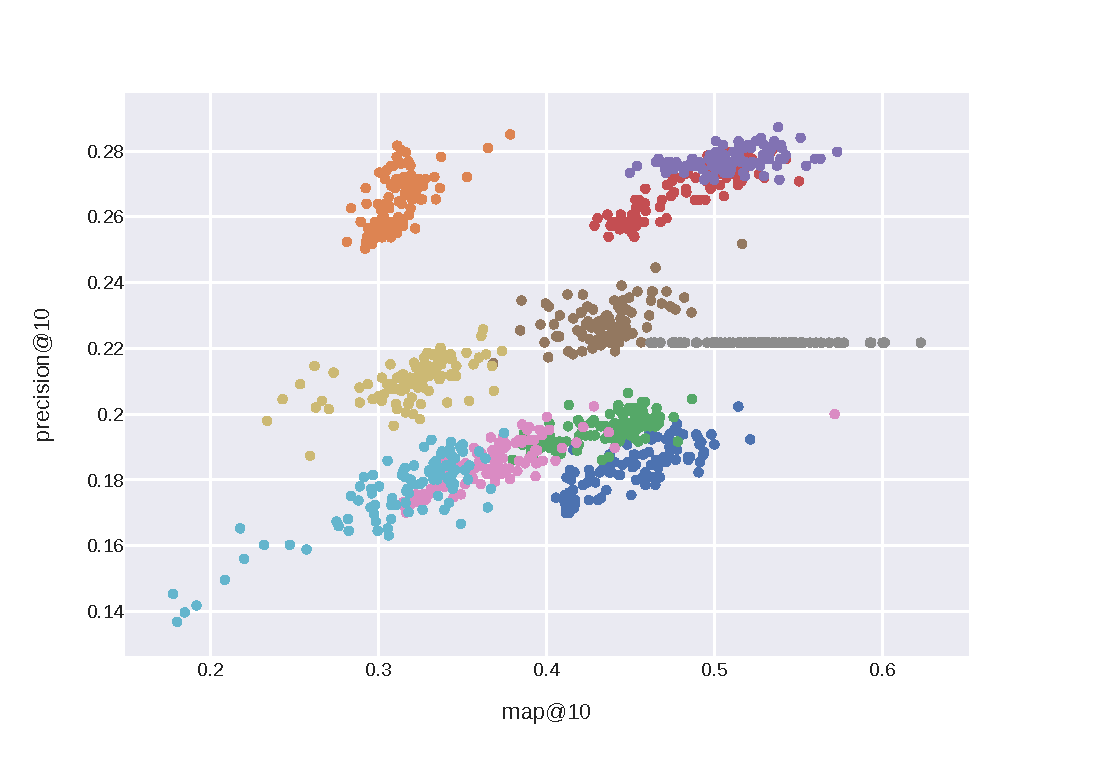
\includegraphics[width=\linewidth]{figures/04_implementacion/scatter_map_precision.pdf}
        \caption[Gráfico de dispersión entre el MAP y la precisión en las 1000 muestras tomadas del recomendador GNN para Decentraland.]{Gráfico de dispersión entre el \gls{map} y la precisión en las 1000 muestras tomadas para la optimización del recomendador basado en \gls{gnn} para la \gls{dao} Decentraland. Dentro de cada fold (color), aumentar el \gls{map} hace aumentar la precisión.}
        \label{fig:scatter_map_precision}
    \end{minipage}%
    \hfill%
    \begin{minipage}{.48\textwidth}
        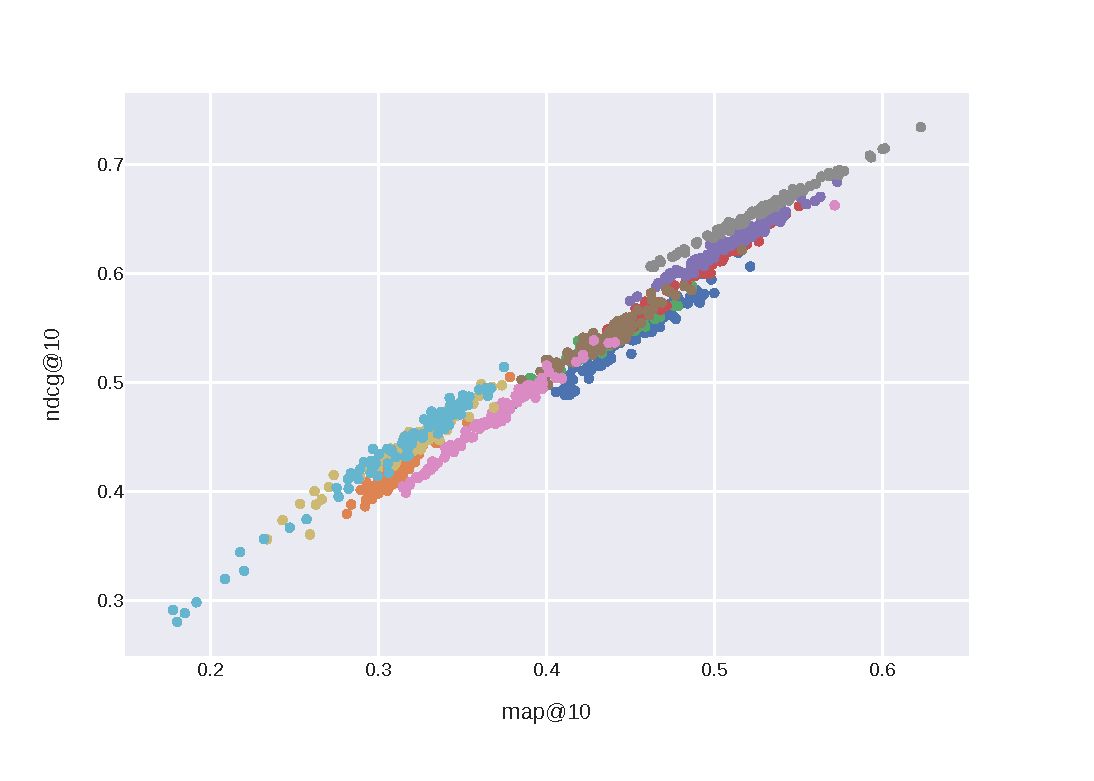
\includegraphics[width=\linewidth]{figures/04_implementacion/scatter_ndcg_map.pdf}
        \caption[Gráfico de dispersión entre el MAP y el nDCG en las 1000 muestras tomadas del recomendador GNN para Decentraland.]{Gráfico de dispersión entre el \gls{map} y el \gls{ndcg} en las 1000 muestras tomadas para la optimización del recomendador basado en \gls{gnn} para la \gls{dao} Decentraland. El color es distinto para cada uno de los folds, mostrando que cada fold tiene unas métricas máximas alcanzables distintas.}
        \label{fig:scatter_ndcg_map}
    \end{minipage}
\end{figure}

Todo el trabajo realizado se encuentra documentado en dos notebooks disponibles en el repositorio de GitHub del proyecto~\cite{davo_daviddavoupm-tfm-notebooks_2024}. El primero, denominado \url{07\_microsoft\_tuning.ipynb}, aborda la definición del proceso de entrenamiento del modelo. El segundo, \url{09\_analyze\_results}, presenta los resultados de la ejecución y genera las métricas y gráficas expuestas en las siguientes secciones.

La decisión de utilizar dos notebooks se tomó para permitir la ejecución en paralelo del segundo y monitorizar el estado de ejecución del primero, ya que el experimento en su totalidad requiere varias horas para completarse.

\subsubsection{Tiempo de ejecución}

El experimento se configura para realizar 100 muestras en 10 folds, con cada ejecución limitada a 5 minutos (300 segundos). Por ende, el tiempo de ejecución teórico asciende a 5,000 minutos, aproximadamente 3 días y medio. No obstante, en la práctica, la suma de los tiempos de ejecución de los experimentos es de 3 días y 20 horas. Esto se debe a que, en lugar de interrumpir abruptamente el experimento, se permite que no continúe tras concluir el \textit{epoch}, y el tiempo medio de ejecución se sitúa en 330 segundos.

El tiempo real de ejecución del experimento es de aproximadamente 5 horas y 45 minutos. Esto se debe a que el servidor utilizado (consultar el apéndice~\ref{ch:servidor}) permitía la ejecución de 16 entrenamientos en paralelo sin afectar el tiempo de ejecución de otros entrenamientos. 

\subsubsection{Emisiones del experimento}
Según la información proporcionada por el programa nvidia-smi, la tarjeta gráfica consumía 250W durante la ejecución de los experimentos. Además, de acuerdo con las especificaciones del procesador~\cite{intel_procesador_2022}, este tiene una potencia base de 150W, aunque no se estaba utilizando al 100\%.

Por lo tanto, la ejecución del experimento consumió 2.3KWh, equivalente a 0.23KWh por cada \textit{fold} como cota superior. En términos de emisiones, actualizar las recomendaciones resultaría en una emisión de 630g de $CO_2$ al utilizar una comercializadora en España sin \gls{gdo}~\cite{noauthor_anexo_2023}. En caso de actualizar las recomendaciones semanalmente, las emisiones ascenderían a aproximadamente 33kg de $CO_2$. Cabe destacar que, al ubicarse el servidor en la Facultad de Informática de la Universidad Complutense de Madrid, que ha adoptado electricidad de origen verde desde 2019, no se generan emisiones~\cite{vicerrectorado_de_tecnologia_y_sostenibilidad_informe_2021}.

\subsubsection{Evaluación del modelo}

No podemos emplear una búsqueda de hiperparámetros calculando el promedio de los resultados de todos los folds, ya que implicaría asumir dos supuestos cruciales: en primer lugar, que todos los modelos de cada fold deben tener los mismos hiperparámetros; y en segundo lugar, que los resultados de cada fold estarían disponibles para evaluar los anteriores.

Por lo tanto, optamos por realizar la optimización de hiperparámetros de manera independiente en cada fold. De las 100 muestras obtenidas durante la ejecución de la optimización de hiperparámetros de un fold, seleccionamos la mejor y la evaluamos utilizando dichos hiperparámetros en el siguiente fold.

Esta metodología busca simular el comportamiento de la optimización de hiperparámetros en un entorno real, donde se dispone de los datos hasta el momento actual pero se desconocen los datos futuros. Por ende, optimizamos los hiperparámetros utilizando únicamente los datos disponibles hasta el momento.

Es crucial resaltar que, para calcular la métrica objetivo de la optimización de hiperparámetros, utilizamos un conjunto de validación que, supuestamente, no está disponible en el momento del entrenamiento. Por esta razón, al modelo optimizado le llamamos \textquote{Oráculo}. Al modelo que emplea los hiperparámetros que obtienen la mejor métrica en el \textit{Oráculo} del fold anterior, lo denominamos \textquote{Realista}.

% https://en.wikibooks.org/wiki/LaTeX/Floats,_Figures_and_Captions
\begin{wrapfigure}{o}{.5\textwidth}
    \centering
    % Source: 09_analyze_results.ipynb [29]
    % Actualizado: 2024-04-10
    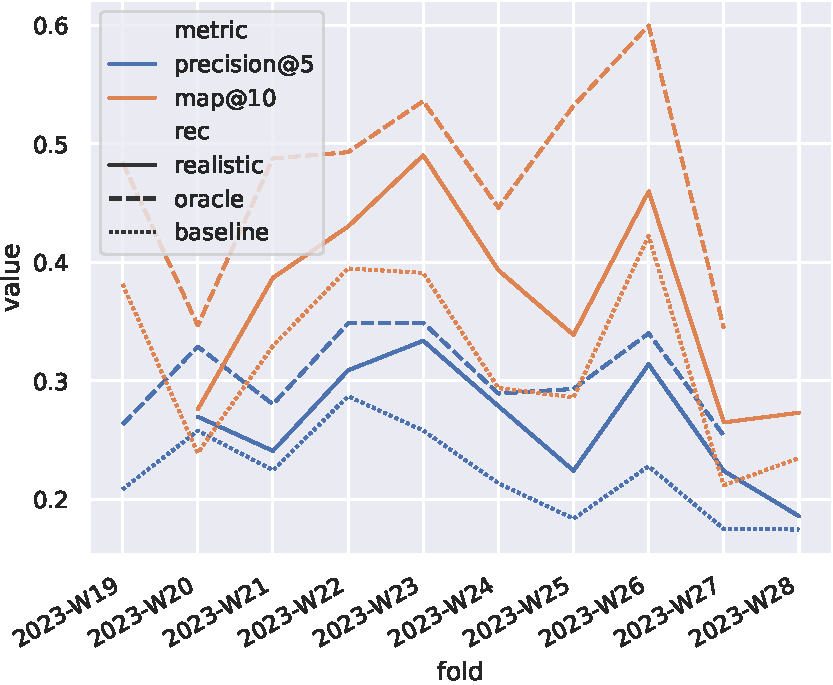
\includegraphics[width=\linewidth]{figures/04_implementacion/09_gnn_results.pdf}
    \caption[Resultados del entrenamiento realista del Sistema Recomendador basado en \textit{Graph Neural Networks}]{Resultados del entrenamiento \textit{realista} del \gls{sr} basado en \gls{gnn}.}
    \label{fig:gnn-realistic}
\end{wrapfigure}

% Source: 09_analyze_results.ipynb [29]
% Actualizado: 2024-04-10
En la figura~\ref{fig:gnn-realistic} se exponen los resultados de estas operaciones en los últimos 10 folds, comparando estos modelos con una línea base (recomendar las propuestas más votadas hasta el momento, véase~\ref{sec:linea_base}). La línea base arroja una MAP@10 media de $0.32\pm0.08$, mientras que el modelo Oráculo está altamente optimizado con un valor medio de $0.47\pm0.08$. El modelo Realista se posiciona entre ambos, con un valor de $0.37\pm0.08$. Aunque siempre es preferible utilizar el modelo Oráculo, el modelo Realista demuestra un rendimiento notable al superar en general a la línea base. En el capítulo~\ref{ch:resultados_discusion} se lleva a cabo una comparación entre los resultados obtenidos por el modelo Realista y el basado en \gls{pln} y el enfoque Híbrido.

\subsection{Sistema híbrido}
\label{subsec:implementacion-hybrid}

% \begin{itemize}
%     \item Es un sistema híbrido basado en la combinación de las recomendaciones de los dos sistemas presentados en los apartados anteriores.
%     \item Para la recomendación basada en contenido, se ha utilizado el modelo basado en la similitud del coseno con el embeding del usuario, en lugar del modelo \gls{knn}, debido a sus mejores resultados y rapidez.
%     \item Se han utilizado los hiperparámetros optimizados para los sistemas individuales, no se ha vuelto a realizar una búsqueda de hiperparámetros en el híbrido.
%     \item Para combinar los resultados, se piden $k$ recomendaciones a cada uno de los sistemas, y se entremezclan para formar un conjunto de $k$ recomendaciones. En caso de haber recomendaciones duplicadas, en las que coinciden ambos sistemas, podemos distinguir tres métodos de fusión, que se detallarán en la siguiente sección.
% \end{itemize}

El sistema híbrido propuesto combina las recomendaciones generadas por los dos sistemas presentados en los apartados anteriores. En lugar del modelo \gls{knn} utilizado en la recomendación basada en contenido, se optó por emplear el modelo basado en la similitud del coseno con el \textit{embedding} del usuario, debido a su mejor desempeño y rapidez. Se emplearon los hiperparámetros optimizados para cada sistema individual, Sin realizar una búsqueda adicional de hiperparámetros para el sistema híbrido. El código de este modelo se encuentra en la clase \url{src.models.hybrid.HybridRecommendation}, y se ha evaluado su funcionamiento en el notebook \url{12_hybrid.ipynb}.

Para combinar los resultados de ambos sistemas, se solicitan $k$ recomendaciones a cada uno y se intercalan para formar un conjunto de $k$ recomendaciones. En caso de que existan recomendaciones duplicadas, es decir, aquellas en las que coinciden ambos sistemas, se han definido tres métodos de fusión, que se detallarán en la siguiente subsección. En la figura~\ref{fig:metodos-fusion} ofrece una visualización de estos tres métodos.

\subsubsection{Métodos de fusión}

\begin{figure}[bth]
    \centering
    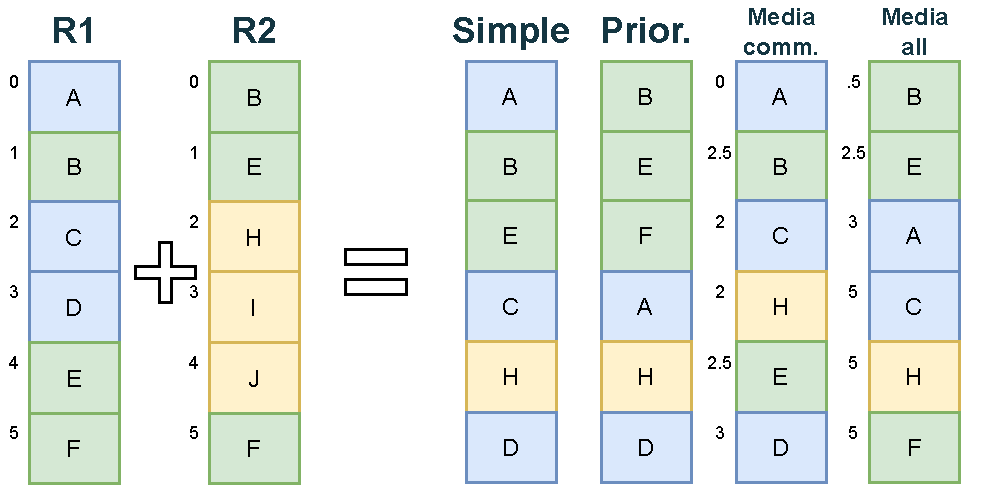
\includegraphics[width=\linewidth]{figures/04_implementacion/metodos-fusion.drawio.pdf}
    \caption[Visualización de los distintos métodos de fusión implementados de dos grupos de recomendaciones.]{Visualización de los distintos métodos de fusión implementados de dos grupos de recomendaciones. En azul las recomendaciones exclusivas al primer recomendador, en amarillo las recomendaciones exclusivas del segundo, y en verde las recomendaciones comunes. Una recomendación superior será una recomendación igual o mejor que la inferior, aunque no son comparables entre recomendadores. El número de la izquierda indica la posición, o el \textit{score} del sistema basado en la posición media.}
    \label{fig:metodos-fusion}
\end{figure}

% \begin{itemize}
%     \item La fusión de los dos sistemas recomendadores está basada en el entrelazamiento de las recomendaciones de ambos. Es decir, se coje una recomendación de cada uno hasta llegar a $k$.
%     \item Sin embargo, según como tratemos a las recomendaciones que aparecen en ambos, podemos distinguir tres métodos, que puede visualizarse su funcionamiento en la figura~\ref{fig:metodos-fusion}.
% \end{itemize}

La fusión de los dos sistemas recomendadores se basa en el entrelazamiento de las recomendaciones de ambos, es decir, se selecciona una recomendación de cada sistema hasta alcanzar $k$. Sin embargo, la manera en que tratamos las recomendaciones que aparecen en ambos sistemas puede variar, y a continuación se describen cuatro métodos de tratar estos duplicados:


\paragraph*{Entrelazado simple}

Se realiza el entrelazado de las recomendaciones y luego se eliminan los elementos duplicados. Es decir, la prioridad asignada a un elemento común será la máxima de las prioridades generadas por los dos recomendadores.

\paragraph*{Priorizar los comunes}

Se priorizan primero los elementos comunes, asumiendo que si ambos recomendadores coinciden en una recomendación, es porque se considera una buena opción. Los elementos no comunes, son entrelazados.

\paragraph*{Posición media de los comunes}

Se calcula la posición media de los elementos comunes en ambos sistemas, y luego se seleccionan los elementos según su \textit{ranking} en esta posición media. Los elementos que no son comunes no varían su \textit{puntuación}. Un elemento duplicado que aparece en la primera posición de un recomendador y en la tercera del otro, tendrá una puntuación de 1, por lo que debería aparecer entre el primero y el segundo.

\paragraph*{Posición media}

% \begin{itemize}
%     \item Las recomendaciones que aparezcan en un solo recomendador seguramente no sean tan buenas. 
%     \item Por lo tanto, también se hace la media de sus posiciones, pero como no conocemos la posición en la que está en el otro recomendador, asumimos que estaría en la posición $i+k$ del otro recomendador.
%     \item Es decir, la posición de los comunes es la media, y la de los no comunes es penalizada sumandole $k/2$
% \end{itemize}

Al igual que en el método anterior, se calcula la posición media de los elementos comunes entre ambos sistemas. Sin embargo, como asumimos que las recomendaciones que no aparecen en ambos sistemas puede que no sean tan buenas, también se calcula su posición media. Como no se conoce la posición real en el otro recomendador, se asume que estarían en la posición $i+k$, donde $i$ es la posición en el recomendador en el que aparecen, y $k$ es el número de elementos comunes. Es decir, se penaliza la posición de los elementos no comunes agregándoles $k/2$ a su posición.

\subsubsection{Evaluación del recomendador híbrido}

% \begin{itemize}
%     \item El sistema híbrido combina los resultados de ambos así que, seguramente, más que mejorar, conseguirá una métrica intermedia, pero probablemente más estable.
%     \item Conforme se va aumentando la $k$ del número de recomendaciones, aparecen más recomendaciones repetidas y, por lo tanto, el método de fusión será cada vez menos relevante. Sin embargo, de realizar 5 recomendaciones, el 50\% serán exclusivas de cada recomendador, como puede verse en la figura~\ref{fig:hybrid-common-proposals}.
%     \item Como puede verse en la figura~\ref{fig:hybrid-fusion-results}, el método de fusión que más beneficia a los comunes es, obviamente, el que prioriza a los comunes. Además, todos los métodos benefician ligeramente (hasta en $1/k$) al recomendador basado en \gls{pln}, pues cuando se hace el entremezclado, siempre se empieza por este y puede haber uno más.
%     \item Por cierto, el método que hace la media solo con los comunes y el del entrelazado puro (\textit{naive}) parece que tienden a escoger poco las recomendaciones comunes.
%     \item Además, con 10 recomendaciones se suelen coger tantas recomendaciones comunes que el método de fusión a penas afecta en que recomendador se elige.
%     \item Debido a que el recomendador basado en contenido es ligeramente mejor que el otro, el mejor método será el que priorice a este, aunque debido a la gran cantidad de recomendaciones comunes, saldrán resultados similares.
%     \item En la tabla \ref{tab:hybrid-fusion-results} podemos ver los resultados de los cuatro métodos, donde se observa que el mejor es el \textit{naive} por poco, ya que es el que más utiliza los resultados del nlp. Parece ser que, de hecho, podría ser mejor utilizar los resultados del nlp no-comunes y penalizar los comunes, ya que el recomendador basado en \gls{gnn} es peor.
%     \item En la figura~\ref{fig:hybrid-fusion-results-folds} se muestran los resultados de cada uno de los métodos fold a fold. El mejor método varía mucho dependiendo de como sean los datos de entrada, pero aun así excepto \textit{prioritize}, que parece más alocado, todos van de la mano y son similares.
% \end{itemize}

El enfoque híbrido propuesto combina los resultados de los \glspl{sr} basados en contenido y en filtrado colaborativo, buscando alcanzar un equilibrio entre ambos enfoques. Este método podría proporcionar un resultado intermedio entre los resultados individuales de cada sistema, aumentando la estabilidad de las recomendaciones.

Al incrementar el número de recomendaciones generadas ($k$), es probable que aumente la cantidad de recomendaciones duplicadas entre los sistemas. A medida que se generan más recomendaciones, disminuye la relevancia del método elegido para fusionar los dos sistemas. Con tan sólo 5 recomendaciones, el 50\% son comunes entre ambos sistemas, y con 10 este número aumenta al 74\%, como se puede observar en la figura~\ref{fig:hybrid-common-proposals}. De hecho, la precisión solo varía en una centésima según el método elegido (tabla~\ref{tab:hybrid-fusion-results}). Sin embargo, sí que será relevante la manera en la que se ordenan estas recomendaciones comunes para el \gls{map} y el \gls{ndcg}.

% LAS DOS FIGURAS LADO A LADO
% \begin{figure}
%     \begin{minipage}{.48\textwidth}
%         \centering
%         \includegraphics[width=\linewidth]{figures/04_implementacion/12_hybrid_common__Decentraland_W-THU_normalize=True.pdf}
%         \caption{Porcentaje de propuestas en común entre el recomendador basado en contenido y el de filtrado colaborativo aumentando el número de recomendaciones.}
%         \label{fig:hybrid-common-proposals}
%     \end{minipage}%
%     \hfill%
%     \begin{minipage}{.48\textwidth}
%         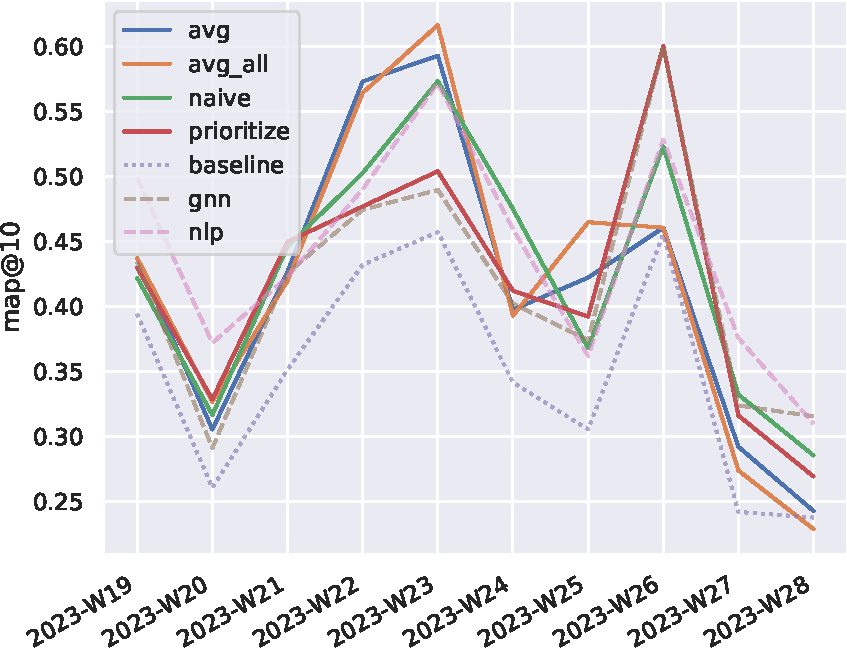
\includegraphics[width=\linewidth]{figures/04_implementacion/12_hybrid_merge_results_folds_Decentraland_W-THU_normalize=True.pdf}
%         \caption{Resultados del sistema recomendador híbrido que usa los distintos métodos de fusión en cada fold.}
%         \label{fig:hybrid-fusion-results-folds}
%     \end{minipage}
% \end{figure}

% SIDE CAPTION
\begin{SCfigure}
    \centering
    \caption[Porcentaje de propuestas en común entre los dos recomendadores base.]{Porcentaje de propuestas en común entre el recomendador basado en contenido y el de filtrado colaborativo aumentando el número de recomendaciones.}
    % Source: 12_hybrid.ipynb [20]
    % Actualizado: 2024-04-10
    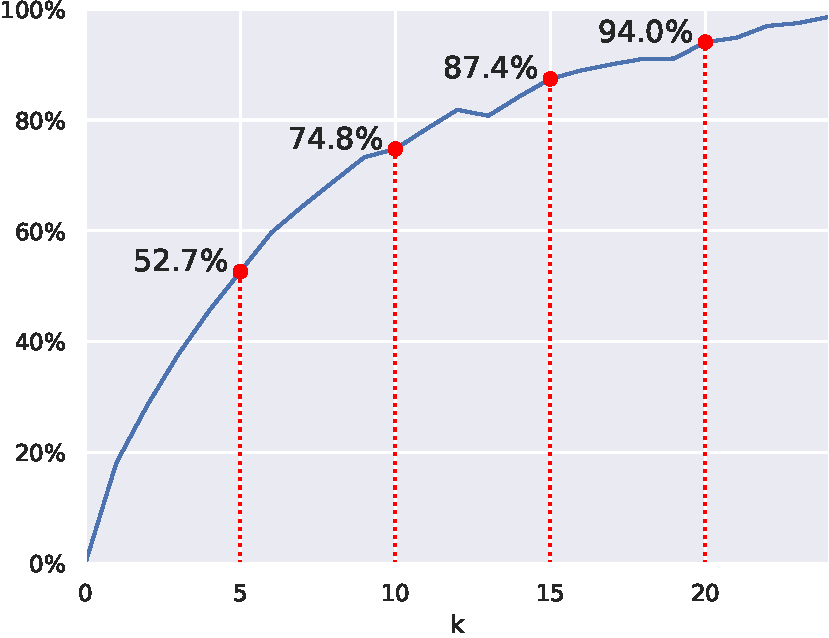
\includegraphics[width=.4\linewidth]{figures/04_implementacion/12_hybrid_common_Decentraland_W-THU_normalize=True.pdf}
    \label{fig:hybrid-common-proposals}
\end{SCfigure}
\begin{table}
    \centering
    \small
    % 12_hybrid.ipynb [25]
    % Actualizado: 2024-04-10
    \begin{tabular}{@{} l *{8}{S[table-format=1.3]} @{}}
        \toprule
          & 
         \multicolumn{2}{c}{precision@k} & 
         \multicolumn{2}{c}{recall@k} &
         \multicolumn{2}{c}{MAP@k} &
         \multicolumn{2}{c}{nDCG@k}
         \\
        % \cmidrule(r{5pt}){2-3}\cmidrule(l{5pt}){4-5}
        \textbf{Model} & 
        \multicolumn{1}{c}{k=5} & 
        \multicolumn{1}{c}{k=10} & 
        \multicolumn{1}{c}{k=5} & 
        \multicolumn{1}{c}{k=10} & 
        \multicolumn{1}{c}{k=5} & 
        \multicolumn{1}{c}{k=10} & 
        \multicolumn{1}{c}{k=5} & 
        \multicolumn{1}{c}{k=10}
        \\
        \midrule
         % avg & 0.416 & 0.113 & 0.360 & 0.095 \\
         % avg\_all & 0.417 & 0.122 & 0.357 & 0.087 \\
         % naive & \textbf{0.435} & \textbf{0.097} & \textbf{0.365} & \textbf{0.087} \\
         % prioritize & 0.431 & 0.106 & 0.357 & 0.093 \\ \hline
         % baseline & 0.348 & 0.085 & 0.274 & 0.074 \\
         % gnn & 0.425 & 0.010 & 0.352 & 0.097 \\
         % nlp & 0.439 & 0.084 & 0.364 & 0.083 \\

         % PRE 2024-04-10
        %  avg & 0.416 & 0.113 & 0.360 & 0.095 & 0.229 & 0.041 & 0.296 & 0.058 \\
        % avg\_all & 0.417 & 0.122 & 0.357 & 0.087 & 0.227 & 0.042 & 0.297 & 0.056 \\
        % naive & \textbf{0.435} & 0.097 & \textbf{0.365} & 0.087 & 0.228 & 0.042 & 0.298 & 0.057 \\
        % prioritize & 0.431 & 0.106 & 0.357 & 0.093 & 0.228 & 0.041 & 0.299 & 0.058 \\ \hline
        % baseline & 0.348 & 0.085 & 0.274 & 0.074 & 0.203 & 0.036 & 0.242 & 0.047 \\
        % gnn & 0.425 & 0.100 & 0.352 & 0.097 & 0.223 & 0.040 & 0.288 & 0.055 \\
        % pln & 0.439 & 0.084 & 0.364 & 0.083 & 0.229 & 0.040 & 0.299 & 0.066 \\
 OpenPop    & 0.221 & 0.196 & 0.351 & 0.626 & 0.236 & 0.310 & 0.317 & 0.416 \\
 \hline
 avg. all   & 0.292 & 0.222 & 0.526 & 0.751 & 0.347 & 0.398 & 0.458 & 0.515 \\
 avg.       & 0.287 & 0.224 & 0.514 & 0.759 & 0.341 & 0.399 & 0.449 & 0.518 \\
 prioritize & 0.291 & 0.224 & 0.525 & 0.755 & 0.341 & 0.399 & 0.452 & 0.520 \\
 naive      & 0.289 & 0.224 & 0.521 & 0.757 & 0.353 & 0.426 & 0.460 & 0.540 \\
 \hline
 GNN        & 0.271 & 0.216 & 0.485 & 0.736 & 0.334 & 0.409 & 0.434 & 0.522 \\
 NLP        & 0.295 & 0.227 & 0.513 & 0.765 & 0.357 & 0.434 & 0.464 & 0.549 \\
    \bottomrule
    \end{tabular}
    \caption{Resultados media de los distintos métodos de fusión del sistema recomendador híbrido y comparación con línea base y los otros dos sistemas recomendadores.}
    \label{tab:hybrid-fusion-results}
\end{table}

Todos los métodos benefician ligeramente al sistema basado en \gls{pln}, debido a que es seleccionado primero durante el entrelazado en el proceso de fusión, como puede verse en la figura~\ref{fig:hybrid-fusion-results}. Debido a que este es el mejor sistema de los dos, el método que más priorice las propuestas del \gls{pln} sobre las otras dará mejores resultados. El método que más elige las propuesas comunes es, obviamente, \textit{prioritize}, seguido de avg\_all, los dos métodos pesimistas sobre las recomendaciones realizadas por uno solo de los sistemas. Parece que el mejor de todos es \textit{naive}, que podríamos considerar que en lugar de agregar utilizando la operación \textit{media} utiliza la operación \textit{máximo}. Puede que este sea el mejor método (tabla~\ref{tab:hybrid-fusion-results}) porque tiende un poco más a escoger propuestas del recomendador \gls{pln}. Como puede verse en la figura, al aumentar el número de recomendaciones de 5 a 10, el método de fusión es menos relevante, pues siempre hay más de un 65\% de recomendaciones en común.

Finalmente, como se puede observar en la tabla~\ref{tab:hybrid-fusion-results} el recomendador híbrido tiene unos resultados entre medias de los dos recomendadores que lo forman, aunque en el map@5 supera al pln por una centésima.

Sin embargo, como se puede ver en la figura~\ref{fig:hybrid-fusion-results-folds} en el fold W19 el método \textit{proritize} supera al naive en map@10, y en los folds W22 y W23 es el \textit{avg} el que lo supera. Por lo tanto, el sistema recomendador híbrido podría superar a ambos de elegir de mejor manera cual de los dos sistemas base priorizar. La figura~\ref{fig:hybrid-best-results-folds} muestra los resultados de el mejor de los híbridos y los compara con los otros sistemas. El sistema \textit{naive}, que obtiene los mejores resultados de media, se encuentra entre los resultados del modelo GNN y el NLP excepto en el fold W23. En esta figura también se muestra con un sombreado azul los mejores y peores resultados obtenido por cualquier método de fusión, y en este caso sí que se supera en varios folds al modelo NLP. De hecho, de escoger en cada caso el mejor método de fusión, se conseguiría un MAP@10 medio de 0.437, superando en 3 centésimas al modelo NLP y demostrando que una mejor hibridación podría llegar a superar los resultados de ambos modelos base desarrollados.

\begin{figure}
    \centering
    % Source: 12_hybrid.ipynb [30]
    % Actualizado: 2024-04-10
    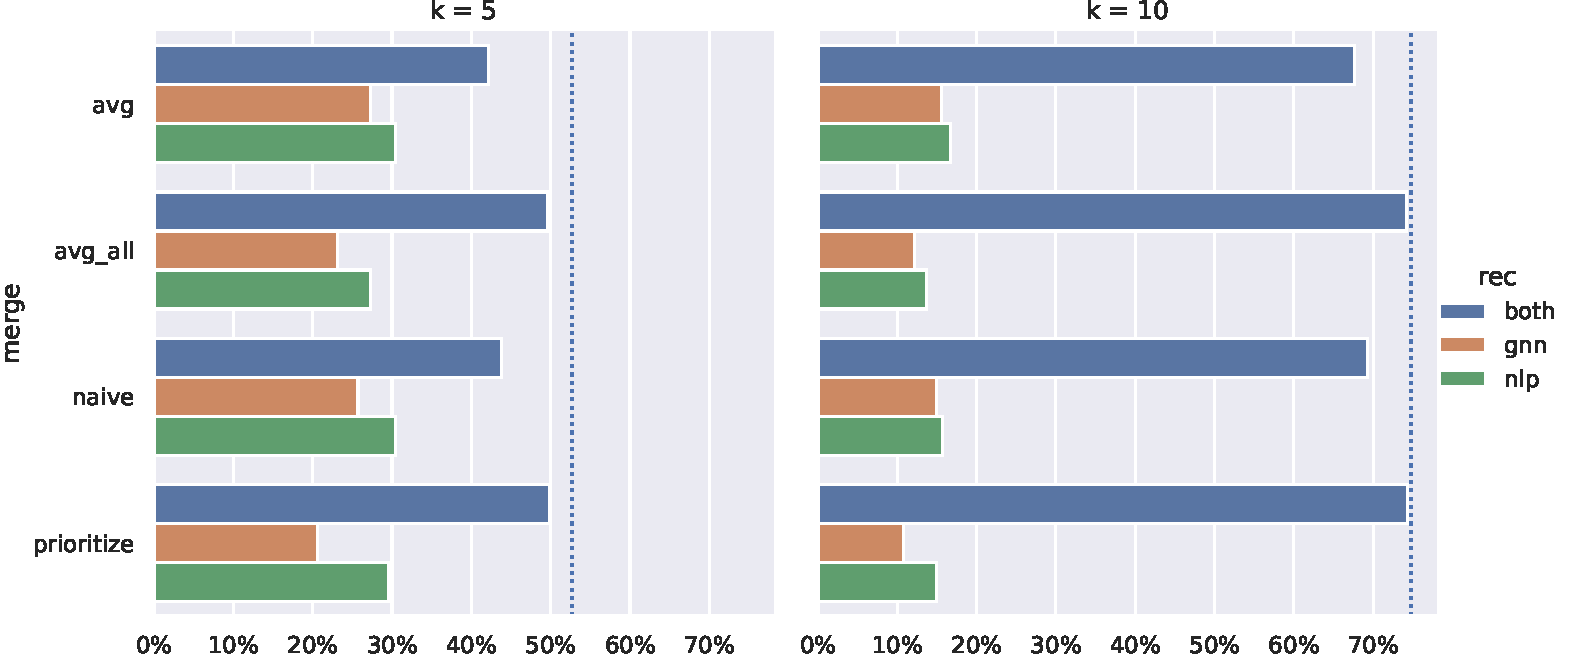
\includegraphics[width=\linewidth]{figures/04_implementacion/12_hybrid_merge_usage_Decentraland_W-THU_normalize=True.pdf}
    \caption[Porcentaje de propuestas de cada recomendador elegidas por cada uno de los métodos de fusión del recomendador híbrido.]{Porcentaje de propuestas de cada recomendador elegidas por cada uno de los métodos de fusión del recomendador híbrido (media de todos los folds). En las 5 recomendaciones originales, el porcentaje de propuestas duplicadas es 50.6\%, y con 10 recomendaciones hay un 74\% de propuestas duplicadas.}
    \label{fig:hybrid-fusion-results}
\end{figure}

\begin{figure}[p]
    \centering
    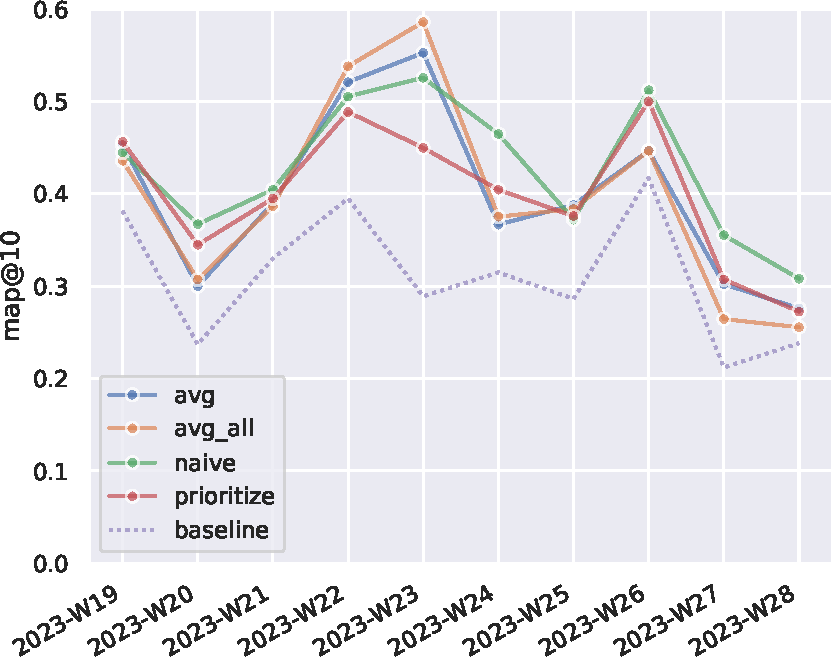
\includegraphics[width=.7\linewidth]{figures/04_implementacion/12_hybrid_merge_results_folds_Decentraland_W-THU_normalize=True_simple.pdf}
    \caption[Resultados del sistema recomendador híbrido que usa los distintos métodos de fusión en cada fold]{Resultados del sistema recomendador híbrido que usa los distintos métodos de fusión en cada fold, comparado con la línea base OpenPop.}
    \label{fig:hybrid-fusion-results-folds}
\end{figure}
\begin{figure}[p]
    \centering
    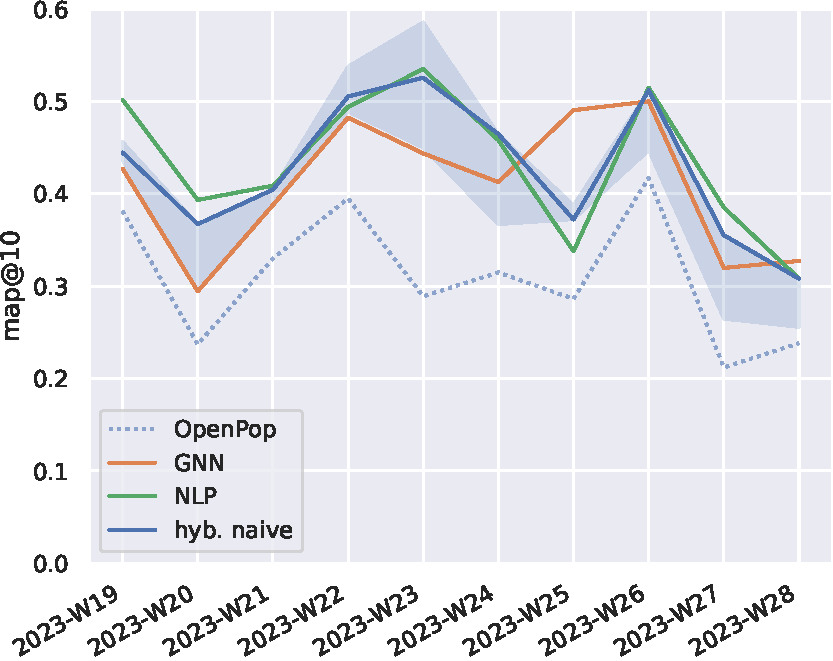
\includegraphics[width=.7\linewidth]{figures/04_implementacion/12_hybrid_merge_results_folds_Decentraland_W-THU_normalize=True_compare.pdf}
    \caption[Comparación del mejor híbrido con otros sistemas recomendadores.]{Resultados del sistema recomendador híbrido \textit{naïve} comparado con los otros sistemas recomendadores desarrollados. El área azul representa el mejor y peor resultado obtenido en ese fold por cualquiera de los otros métodos de fusión.}
    \label{fig:hybrid-best-results-folds}
\end{figure}


% \part{Conclusiones y resultados}
\chapter{Resultados y discusión}
\label{ch:resultados_discusion}

% \section{Resumen de resultados}
% \label{sec:resumen_resultados}

Para desarrollar el modelo se han utilizado las últimas 10 semanas del conjunto de datos de la organización \textit{Decentraland}, que cuenta con 117 mil votos emitidos por 7300 votantes en 1942 propuestas. El modelo se entrena con una división en folds temporales incrementales, por lo que cada semana el número de propuestas y votos en el conjunto de entrenamiento aumenta, aunque solo se utilizan para evaluación las propuestas que están abiertas en el momento de hacer el split, como se detalla en la sección~\ref{sec:division_datos}.

Los resultados fold a fold del entrenamiento de los modelos pueden consultarse en el capítulo~\ref{ch:implementacion_experimentos}. Tras desarrollar el modelo usando Decentraland como objetivo, se ha seguido el proceso para \glspl{dao} seleccionadas de la tabla~\ref{tab:4_daos_relevantes}. Para seleccionar las organizaciones, se han eliminado las organizaciones marcadas como SPAM en su plataforma. Además, se ha explorado el conjunto de datos para observar cual es la distribución de la duración de las propuestas, y se han realizado las recomendaciones de manera acorde.

\begin{table}[b]
\centering
\begin{threeparttable}[t]
    \footnotesize
    % Generado en 04b_dao-census-text.ipynb
    \begin{tabular}{l|cc}
        \toprule
        \textbf{Nombre} &
        \textbf{Entrenamiento} &
        \textbf{Fecha últ. fold} \\
        \midrule
        Decentraland & Semanal (Jueves) & 2023-07-28\tnote{\textdagger} \\
        % Balancer NO
        DEAD Foundations DAO & Cada 2 días & 2021-11-28 \\
        % dxDAO / xDXdao & 5 días & NO \\
        % Index Coop & 2 días & 2022-01-01 & NO \\ 
        MetaCartel / MetaCartel Ventures & Semanal (Jueves) & 2022-07-22 \\
        PancakeSwap & Cada 3 días & 2023-07-01 \\
        Aave / Aavegotchi & Cada 5 días & 2023-07-28\tnote{\textdagger} \\
        \bottomrule
    \end{tabular}
    \begin{tablenotes}
        \item[\textdagger] Es el último fold disponible en el conjunto de datos.
    \end{tablenotes}
    \caption{Organizaciones sobre las que se han entrenado los modelos.}
    \label{tab:7_daos_entrenadas}
\end{threeparttable}
\end{table}

En el caso de Decentraland, se utilizan los últimos 10 folds disponibles. Sin embargo, esto no es posible en todas las organizaciones, por lo que se ha buscado un rango de fechas tal que los folds tengan cierta cantidad de propuestas abiertas. Algunas organizaciones, aún teniendo muchas propuestas, no cumplen estas condiciones, por lo que tampoco se ha ejecutado el sistema recomendador en ellas. Finalmente, las DAOs con las que se ha probado el modelo quedan reflejadas en la tabla~\ref{tab:7_daos_entrenadas}. En cuanto a Aave, no ha sido posible realizar el experimento debido a que cuenta con demasiadas propuestas. Para probar cada una de las organizaciones se ha creado el Jupyter Notebook \url{31_run_all.ipynb}, que ejecuta los notebooks necesarios para cada una de las DAOs seleccionadas. Los resultados de ejecución de dichos notebooks están disponibles en el GitHub del proyecto~\cite{davo_daviddavoupm-tfm-notebooks_2024}, bajo la carpeta \url{nbout}.

% Actualizado 2024-01-22 con W-THU-normalized
% Estas propuestas han tenido interacciones tanto antes como después del corte que discierne si los votos son de entrenamiento o evaluación, y se muestra en la tabla~\ref{tab:open_proposals} el número de votos en dichas propuestas que pertenecen al conjunto de entrenamiento o de test. Recordemos que el conjunto de entrenamiento, sin embargo, incluye también todas las propuestas que ya han sido cerradas. Puede encontrarse una explicación más exhaustiva del split de los datos en la sección~\ref{sec:division_datos}. Este subconjunto del conjunto de entrenamiento es relevante sobre todo para los recomendadores basados en filtrado colaborativo, pues no se pueden recomendar propuestas recién creadas debido al problema de \textit{cold-start}. % En la figura~\ref{fig:open_proposals} se muestra la evolución de el número de propuestas abiertas, la media es de $17.5\pm4.72$, y su valor mínimo es de 10 y el máximo de 25.

Nótese que debido al bajo número de propuestas \textit{relevantes}, algunas métricas de recuperación de información nunca llegarán a tener un valor de $1$ si el valor de la $k$ no es muy bajo. Para solventar este problema, los clasificadores se comparan no solo entre sí, si no también con un clasificador perfecto que nunca falla (y reporta, por lo tanto, la métrica máxima alcanzable), y un clasificador línea base llamado \textit{OpenPop} que recomienda siempre la propuesta abierta más votada en el momento de realizar la recomendación (véase la sección~\ref{sec:linea_base}).

Tras ejecutar el experimento en las 4 organizaciones seleccionadas, en todas ellas los modelos desarrollados superan la linea base establecida, tanto para el ndcg@10 (figura~\ref{fig:all-results-ndcg}) como para la precisión@5 (figura~\ref{fig:all-results-precision}). En general, el modelo basado en \gls{pln} logra mejores resultados que el basado en GNN o el híbrido.

\begin{figure}[t]
    \centering
    \begin{subfigure}{.24\linewidth}
        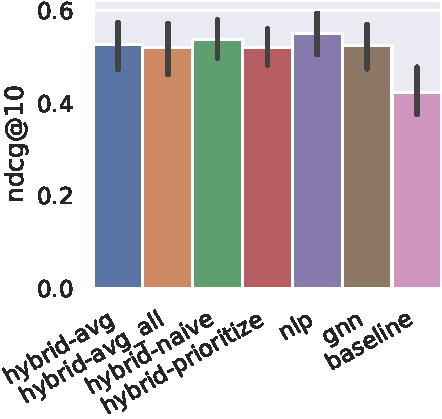
\includegraphics[width=\linewidth]{figures/resultados/7_all-metrics-Decentraland-ndcg@10.pdf}
        \caption{Decentraland}
    \end{subfigure}\hfill\begin{subfigure}{.24\linewidth}
        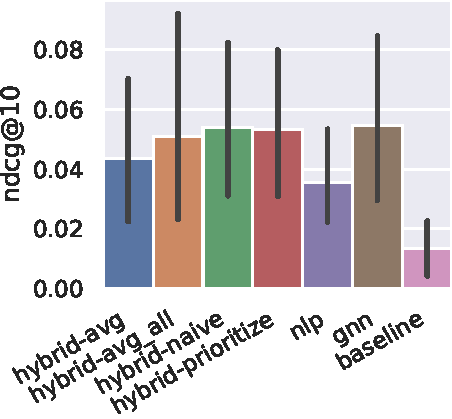
\includegraphics[width=\linewidth]{figures/resultados/7_all-metrics-DEAD FoundationsDAO-ndcg@10.pdf}
        \caption{DEAD Foundations}
        \label{fig:all-results-ndcg-dead_foundation}
    \end{subfigure}\hfill\begin{subfigure}{.24\linewidth}
        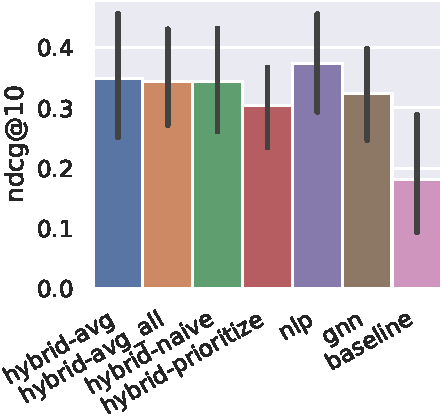
\includegraphics[width=\linewidth]{figures/resultados/7_all-metrics-MetaCartel - MetaCartel Ventures-ndcg@10.pdf}
        \caption{Metacartel}
    \end{subfigure}\hfill\begin{subfigure}{.24\linewidth}
        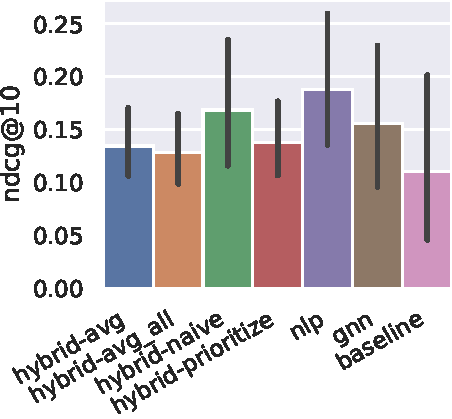
\includegraphics[width=\linewidth]{figures/resultados/7_all-metrics-PancakeSwap-ndcg@10.pdf}
        \caption{PancakeSwap}
    \end{subfigure}
    \caption{Resultados de la métrica ndcg@10 en las organizaciones probadas.}
    \label{fig:all-results-ndcg}
\end{figure}
\begin{figure}[t]
    \centering
    \begin{subfigure}{.24\linewidth}
        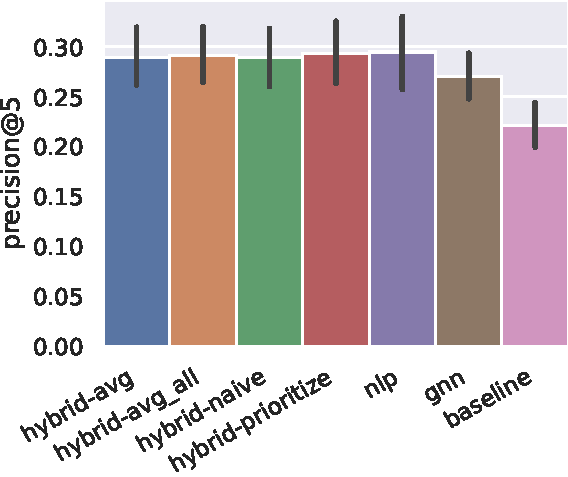
\includegraphics[width=\linewidth]{figures/resultados/7_all-metrics-Decentraland-precision@5.pdf}
        \caption{Decentraland}
    \end{subfigure}\hfill\begin{subfigure}{.24\linewidth}
        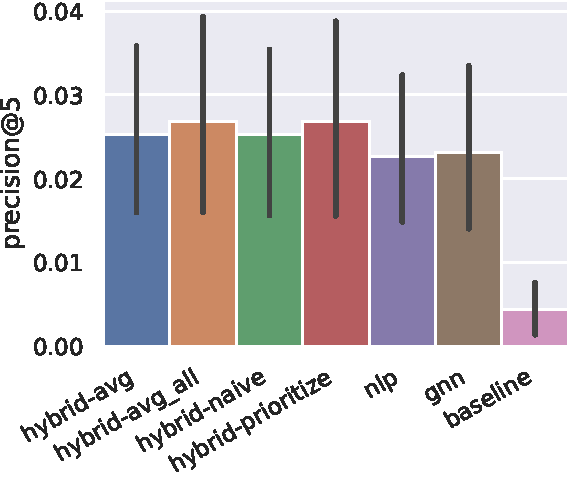
\includegraphics[width=\linewidth]{figures/resultados/7_all-metrics-DEAD FoundationsDAO-precision@5.pdf}
        \caption{DEAD Foundations}
        \label{fig:all-results-precision-dead_foundations}
    \end{subfigure}\hfill\begin{subfigure}{.24\linewidth}
        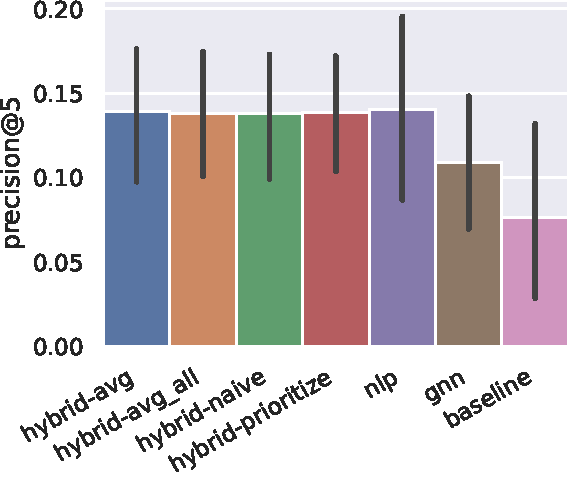
\includegraphics[width=\linewidth]{figures/resultados/7_all-metrics-MetaCartel - MetaCartel Ventures-precision@5.pdf}
        \caption{Metacartel}
    \end{subfigure}\hfill\begin{subfigure}{.24\linewidth}
        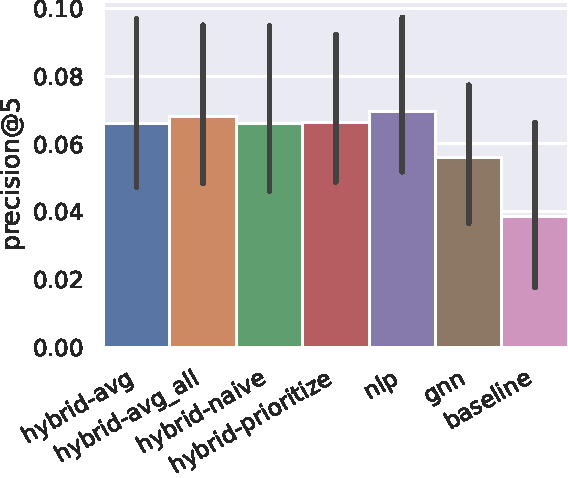
\includegraphics[width=\linewidth]{figures/resultados/7_all-metrics-PancakeSwap-precision@5.pdf}
        \caption{PancakeSwap}
    \end{subfigure}
    \caption{Resultados de la métrica precision@5 en las organizaciones probadas.}
    \label{fig:all-results-precision}
\end{figure}

El modelo GNN, basado en filtrado colaborativo, demuestra el desafío de arranque en frío (\textit{cold-start}) que sufren este tipo de modelos para cada una de las propuestas que se crean continuamente, y que cuentan con pocas interacciones. Como se detalla en la subsección~\ref{subsec:recsys-content}, los sistemas basados en contenido sufren menos dicho problema. Aunque presentan el problema de \textit{cold-start} con usuarios, en este tipo de organizaciones el número de usuarios es relativamente estable.

En cuanto al híbrido, en general logra unos resultados que se sitúan entre el modelo basado en contenido y el basado en filtrado colaborativo. En cuanto a los distintos métodos de fusión de las recomendaciones, las otras organizaciones tienen unas conclusiones similares al caso de Decentraland (véase la subsección~\ref{subsec:implementacion-hybrid}): el método de entrelazado simple parece lograr mejores resultados de \textit{ranking} porque prioriza el PLN, que es el mejor modelo.

La única excepción de entre las organizaciones usadas es DEAD Foundations, en el que el sistema híbrido supera al basado en GNN, que a su vez supera al basado en contenido. 
Esta DAO, además, cuenta con una línea base especialmente baja, y es de hecho la organización con menor densidad ($\simeq2\permil$), como se muestra en la tabla~\ref{tab:4_daos_relevantes}. Este hecho podría indicar que un enfoque híbrido es el camino a seguir para realizar mejores recomendaciones en organizaciones dispersas, que sí que pueden contar con ambos problemas de \textit{cold-start}.

Aunque en todas las organizaciones probadas se supere la linea base, es necesario considerar el contexto específico de cada organización para seleccionar o desarrollar el mejor enfoque de recomendación, analizando su actividad y las características de los usuarios y las propuestas. 

\chapter{Conclusiones y trabajo futuro}

\section{Conclusiones}

Para realizar este trabajo, se ha definido el problema de la recomendación de propuestas en DAOs, y se han creado distintos elementos para evaluar este problema de manera agnóstica al modelo, usando datos históricos (evaluación offline): una línea base robusta inspirada en MostPop acorde a este caso de uso llamada OpenPop, y una manera de realizar validación cruzada con distintos subconjuntos de datos del conjunto de datos, basada en el tiempo.

Para comprobar dicha metodología, se han desarrollado tres sistemas recomendadores: un primer sistema, basado en el contenido, utilizando \textit{embeddings} de la información textual de las propuestas; un segundo de filtrado colaborativo basado en LightGCN; y un tercer recomendador, híbrido, que fusiona los otros dos. Los tres sistemas han superado satisfactoriamente la linea base establecida, siendo el basado en contenido el que mejores resultados ha obtenido, y obteniendo el híbrido resultados entre medias de los otros dos.

Finalmente, se ha comprobado la metodología con otras 3 organizaciones, superando en todas ellas la línea base establecida.

\subsection{Limitaciones}

Debido a que se ha utilizado evaluación offline, desconocemos cómo funcionaría el sistema en un entorno real, y si este afectaría al comportamiento de los usuarios. Aunque en otros tipos de comunidades en línea haya aumentado la participación, no tiene por que ser así en este caso. Además, se han utilizado pocos datos de los presentes en el conjunto de datos.

En el caso del modelo basado en GNN (y, por lo tanto, el híbrido también), deben ser reentrenados para realizar recomendaciones, con sus debidos costes. No se ha comprobado el comportamiento de utilizar en el siguiente fold temporal un modelo preentrenado.

Dentro de la evaluación offline, no se han comprobado métricas que pueden proporcionar información más interesante para explicar las recomendaciones realizadas, como la diversidad, la novedad, serendipia, o la \textit{explained variance}. Además, la diferencia entre la linea base OpenPop, sin personalización, y el resto de modelos probados es muy baja, pues los pocos elementos más votados sesgan las métricas basadas en \textit{top-k recommendations}~\cite{cremonesi_performance_2010}.

\subsection{Trabajo publicado}

El código realizado está disponible en GitHub~\cite{davo_daviddavoupm-tfm-notebooks_2024}, y el conjunto de datos en Kaggle~\cite{tfm-dataset-text}. Los resultados de la búsqueda y optimización de hiperparámetros de los modelos (\url{ray_results}) están disponibles en Zenodo~\cite{tfm-ray-results}.

Finalmente, se ha escrito y enviado un artículo para el \textit{18th ACM Conference on Recommender Systems}, aún pendiente de revisión~\cite{davo_enhancing_2024}.

\section{Trabajo futuro}

Una vez comprobado que ambos enfoques proporcionan recomendaciones similares, debería explorarse mejor el uso de otros modelos, especialmente híbridos, como pueden ser las Factorization Machines como xDeepFM~\cite{lian_xdeepfm_2018}, o algoritmos de GNN para grafos etiquetados. Como la línea base logra muy buenos resultados a bajo coste, podría explorarse el uso de modificaciones con personalización como TimePop~\cite{azzopardi_local_2019}. Dado que la información textual parece ser altamente relevante, pueden realizarse recomendaciones utilizando \glspl{llm}~\cite{li_pap-rec_2024}. Como se ha podido ver, las distribución temporal de votos en propuestas no es uniforme, ni según el tiempo absoluto (día de la semana), ni según el tiempo relativo (horas desde que se abrió la propuesta), por lo que debería añadirse esa información contextual al sistema recomendador. El grafo utilizado para el filtrado colaborativo también puede expandirse utilizando interacciones entre los usuarios fuera de la DAO, pues esos datos son accesibles en el blockchain.

Recientemente se ha añadido soporte para sistemas recomendadores en la librería PyTorch Geometric~\cite{fey_fast_2019}, y en su hoja de ruta está el añadir soporte para grafos temporales, por lo que sería buena idea intentar utilizar sus modelos, pero siguiendo utilizando el \textit{framework} de evaluación de Microsoft Recommenders~\cite{argyriou_microsoft_2020}.

Para mejorar la escalabilidad del modelo, deberían poderse realizar recomendaciones sin la necesidad de reentrenarlo completamente, o bien cambiando el tipo de modelo, o bien comprobando el comportamiento del modelo actual a la reanudación del entrenamiento con nuevos datos.

Finalmente, el sistema podría desplegarse de manera descentralizada, en alguna plataforma como Golem Network~\cite{uriarte_blockchain-based_2018}.

% \begin{itemize}
%     \item Sobre todo, no ignorar la característica temporal del problema. Seguramente tenga más sentido recomendar una propuesta recién creada en las últimas horas que una creada hace 5 días. La de 5 días probablemente haya sido vista por el usuario, pero ha decidido ignorarla activamente. Sin embargo, la que se ha creado hace poco puede que no la haya visto. Recientemente añadieron soporte para sistemas recomendadores en la librería PyTorch Geometric, y está en su roadmap añadir soporte para grafos temporales, por lo que sería buena idea intentar utilizar ese modelo, con el framework de microsoft recommenders.
%     \item En el recomendador kNN pln, probar con otros tipos de sampling negativo
%     \item En el filtrado colaborativo, probar con otros tipos de aprendizaje no supervisado (clústering / \textbf{topic modeling}).
%     \item Afinar mejor las muestras negativas distinguiendo si un usuario no podía tan siquiera haber votado en esa propuesta (por ejemplo, porque se creó antes de que él fuese miembro).
%     \item Enriquecer la parte del recomendador de filtrado colaborativo teniendo en cuenta no solo las propuestas en común, si no las interacciones entre ese usuario y otras DAOs, o incluso incluir transacciones de Ethereum en común entre dos usuarios e interacciones en otras dApps.
%     \item Obviamente, probar con otros tipos de sistemas recomendadores, especialmente, con una MF o FM o como se llame
%     \item En el caso del GNN, cambiarlo por un sistema recomendador que no requiera de la creación de un nuevo modelo en cada caso
%     \item Obviamente, integrar el sistema recomendador en la aplicación original, tal vez con un add-on o un fork o algo similar
%     \item Ejecutar el sistema recomendador de manera descentralizada, con alguna plataforma como Golem Network~\cite{uriarte_blockchain-based_2018}.
% \end{itemize}


% \begin{thebibliography}{99}
% \bibitem{P} Publicaciones utilizadas en el estudio y desarrollo del trabajo.
% Hay que utilizar un sistema internacional para referencias bibliográficas, de acuerdo con las indicaciones del tutor. Por ejemplo, el 
% \href{https://www.etsiinf.upm.es/docs/estudios/grado/1475_ieeecitationref.pdf}{\emph{sistema de IEEE}}

% \end{thebibliography}
\sloppy\printbibliography[category=cited]
\addcontentsline{toc}{chapter}{Bibliografía}

% \nocite{*}
% \printbibliography[title={DELETEME: Zoteros sin citar},notcategory=cited,notkeyword={Ignorebib}]

%%---------------------------------------------------------
% Imprimir el glosario
% \printglossaries
\printglossary[type=\acronymtype, style=listsp]
%%-----------------------------------------------
%% Anexos
\appendix
\chapter{Características del servidor dedicado}
\label{ch:servidor}

Todas las ejecuciones se han realizado en un único servidor dedicado asegurándose de que no había ninguna otra tarea intensiva ejecutándose en el momento. Las epecificaciones de dicho servidor, proporcionado por el Instituto de Tecnología del Conocimiento de la Universidad Complutense de Madrid y administrado por el Departamento de Arquitectura de Computadores y Automática, son las siguientes:

\begin{description}
    \item[OS] Ubuntu 22.04 LTS
    \item[Kernel] Linux 5.15
    \item[Placa base] MPG Z690
    \item[CPU] 12th Gen Intel i9-12900KS (24) @ 5.200GHz
    \item[RAM] 128 GB 
    \item[GPU] NVIDIA AD102 (GeForce RTX 4090) 24 GiB VRAM
\end{description}

A este equipo se ha conectado en remoto mediante SSH para ejecutar Jupyter Notebooks usando Jupyter Lab. Se ha utilizado Python 3.9 debido a la dependencia de la librería de Microsoft Recommenders.
 
\end{document}
